\documentclass[12pt,upcase,hidelinks]{mitthesis}

\usepackage{amsmath, amsthm, amssymb}
\usepackage{microtype}
\usepackage{graphicx}
\graphicspath{{./images/}}
\usepackage{multirow}
\usepackage{rotating}
\usepackage{natbib}
\setcitestyle{numbers}
\usepackage{url}
\usepackage{booktabs}
\usepackage{hyperref}		% turns all internal references into hyperlinks
\usepackage{bm}
\usepackage{algorithmic}
\usepackage{chngpage}
\usepackage[resetlabels]{multibib}
\usepackage{comment}

\usepackage[]{pdfpages}

% use fancyhdr, to enable page style stuff (below)
\usepackage{fancyhdr}
\setlength{\headheight}{15.2pt}
\renewcommand{\headrulewidth}{0pt}

\newtheorem{lemma}{Lemma}
\newtheorem{theorem}{Theorem}
\newtheorem{proposition}{Proposition}
\newtheorem{definition}{Definition}
\newtheorem{assumption}{Assumption}


\newcites{New}{Publications}

\pagestyle{plain}

\begin{document}
% Sherman 1
% Revision 1.1  92/04/22  13:08:20  epeisach

% BE SURE TO READ THE UNIVERSITY'S RULES ON WHAT FIELDS ARE REQUIRED OR ENCOURANGED FOR YOUR DEPARTMENT




% If your want to revise something for the first five page, please go to mitthesis.cls 
\title{Automatic Generation of Multiple-Choice Questions}

\author{Cheng Zhang}


% \date{September 2021}
\maketitle

% \pagenumbering{Roman}

% \paragraph{Abstract}
% \begin{abstract}
% 

Over the past few years, there has been a significant amount of research focused on studying the ReLU activation function, with the aim of achieving neural network convergence through over-parametrization. However, recent developments in the field of Large Language Models (LLMs) have sparked interest in the use of exponential activation functions, specifically in the attention mechanism.

Mathematically, we define the neural function $F: \R^{d \times m} \times  \mathbb{R}^d \rightarrow \mathbb{R}$ using an exponential activation function. Given a set of data points with labels $\{(x_1, y_1), (x_2, y_2), \dots, (x_n, y_n)\} \subset \mathbb{R}^d \times \mathbb{R}$ where $n$ denotes the number of the data. Here $F(W(t),x)$ can be expressed as $F(W(t),x) := \sum_{r=1}^m a_r \exp(\langle w_r, x \rangle)$, where $m$ represents the number of neurons, and $w_r(t)$ are weights at time $t$. It's standard in literature that $a_r$ are the fixed weights and it's never changed during the training. We initialize the weights $W(0) \in \mathbb{R}^{d \times m}$ with random Gaussian distributions, such that $w_r(0) \sim \mathcal{N}(0, I_d)$ and initialize $a_r$ from random sign distribution for each $r \in [m]$.

Using the gradient descent algorithm, we can find a weight $W(T)$ such that $\| F(W(T), X) - y \|_2 \leq \epsilon$ holds with probability $1-\delta$, where $\epsilon \in (0,0.1)$ and $m = \Omega(n^{2+o(1)}\log(n/\delta))$. To optimize the over-parametrization bound $m$, we employ several tight analysis techniques from previous studies [Song and Yang arXiv 2019, Munteanu, Omlor, Song and Woodruff ICML 2022]. 

 

% \end{abstract}


% Add this if you want, revise the mitthesis.cls  for adding previous degree
% \prevdegrees{Previous Degree}

% \department{Department of Computer Science}


% \degree{Doctor of Philosophy}
% \degreemonth{May}
% \degreeyear{2022}
% \thesisdate{May 24, 2022}
% \uml{UMass Lowell}
% % this is the university of my out uml committee member. you may want to remove this
% % \bu{Out Reader's affiliation}


% \supervisor{Jie Wang}{Professor}
% % you may need to revise this line, since one of my committee member is from BU.
% % \outreader{Out Reader}{Jie Wang}
% \reader{Yu Cao}{Professor}
% \reader{Karen Lin}{Professor} 

% \chairman{Haim Levkowitz}{Department Chair}


% \begin{signaturepage}
% \end{signaturepage}
% \thispagestyle{empty}

% \newpage


% \maketitle


% copyright page
% \vspace*{\fill}
% \begin{center}
% \noindent\uppercase{Copyright 2022\\
% Cheng Zhang\\
% All rights reserved}
% \end{center}
% \vspace*{\fill}
% \thispagestyle{empty}
% \newpage


% \newpage
% \null
% \vspace{1.5in}
% \begin{center}
%     \textsuperscript{\textcopyright} \large2022 by Cheng Zhang \\
%     \large All rights reserved\\
% \end{center}
% \thispagestyle{empty}

    
% \thispagestyle{empty}
% \mbox{}
% \newpage
% \thispagestyle{empty}

% \pagestyle{plain}
% \newpage
% \pagenumbering{roman}
% \setcounter{page}{4}
% \thispagestyle{empty}


% \begin{abstractpage}
% 

Over the past few years, there has been a significant amount of research focused on studying the ReLU activation function, with the aim of achieving neural network convergence through over-parametrization. However, recent developments in the field of Large Language Models (LLMs) have sparked interest in the use of exponential activation functions, specifically in the attention mechanism.

Mathematically, we define the neural function $F: \R^{d \times m} \times  \mathbb{R}^d \rightarrow \mathbb{R}$ using an exponential activation function. Given a set of data points with labels $\{(x_1, y_1), (x_2, y_2), \dots, (x_n, y_n)\} \subset \mathbb{R}^d \times \mathbb{R}$ where $n$ denotes the number of the data. Here $F(W(t),x)$ can be expressed as $F(W(t),x) := \sum_{r=1}^m a_r \exp(\langle w_r, x \rangle)$, where $m$ represents the number of neurons, and $w_r(t)$ are weights at time $t$. It's standard in literature that $a_r$ are the fixed weights and it's never changed during the training. We initialize the weights $W(0) \in \mathbb{R}^{d \times m}$ with random Gaussian distributions, such that $w_r(0) \sim \mathcal{N}(0, I_d)$ and initialize $a_r$ from random sign distribution for each $r \in [m]$.

Using the gradient descent algorithm, we can find a weight $W(T)$ such that $\| F(W(T), X) - y \|_2 \leq \epsilon$ holds with probability $1-\delta$, where $\epsilon \in (0,0.1)$ and $m = \Omega(n^{2+o(1)}\log(n/\delta))$. To optimize the over-parametrization bound $m$, we employ several tight analysis techniques from previous studies [Song and Yang arXiv 2019, Munteanu, Omlor, Song and Woodruff ICML 2022]. 

 

% \end{abstractpage}

%%%%%%%%%%%%%%%%%%%%%%%%%%%%%%%%%%%%%%%%%%%%%%%%%%%%%%%%%%%%%%%%%%%%%%
% -*-latex-*-




% \chapter*{Acknowledgement}
\addcontentsline{toc}{chapter}{Acknowledgement}
The authors thank Andrzej Kupsc, Sergey Barsuk, Olivier Callot and Wolfgang K{\"u}hn for their contribution on the CDR draft.
%The authors thank the international review committee XXX for their great effort in reading the CDR draft and providing valuable suggestions. 
The STCF working group thanks all 
the colleagues in the world-wide community for many profitable discussions
and expresses gratitude to the Hefei Comprehensive National Science Center for their strong support.  This work is supported by: international 
partnership program of the Chinese Academy of Sciences Grant No. 211134KYSB20200057.
\include{contents}
%\include{preface} 	% Preface is not part of the standard. I invented it for myself. Use it if you want by uncommenting.

	% Redefine the "plain" pagestyle to have pagenum in the header, right
	\fancypagestyle{plain}{
		\fancyhf{}
		\fancyhead[R]{\thepage}
	}

	\setcounter{page}{1}
	\pagenumbering{arabic}
	\pagestyle{plain}
	
\chapter{CFT entanglement}	\label{chapterCFT}

\abstract*{Entanglement entropy in a conformal field theory can be defined as the von Neumann entropy of the reduced density matrix. We review in this chapter the replica trick derivation of CFT entanglement, following the work of Cardy and Calabrese in section \ref{sectionreplicaCFT} and of Holzhey, Larsen and Wilczek in section \ref{sectionThermal}. This follows an introductory section \ref{sectintro} covering the pictorial notation of wave-functionals and density matrices in the path integral formalism, which is also heavily used in section \ref{sectTFD} on the thermofield double construction. }  


Entanglement entropy in a conformal field theory (CFT) can be defined as the von Neumann entropy of the reduced density matrix. We review in this chapter the replica trick derivation of CFT entanglement, following the work of Cardy and Calabrese \cite{Calabrese:2004eu,Calabrese:2009qy,Cardy:2008jc} in section \ref{sectionreplicaCFT} and of Holzhey, Larsen and Wilczek \cite{Holzhey:1994we} in section \ref{sectionThermal}. This follows an introductory section \ref{sectintro} covering the pictorial notation of wave-functionals and density matrices in the path integral formalism, which is also heavily used in section \ref{sectTFD} on the thermofield double construction. 


\section{Wave-functionals and density matrices} \label{sectintro}

 
We start with reviewing\footnote{For more details, see Appendix A of \cite{Polchinski:1998rq} and section 4 of \cite{Hartmanlectures}.} some basic pictorial notation for wave-functionals and density matrices that will be used throughout. 

In a quantum mechanical system with Hamiltonian $H$ and Euclidean action $I$, the transition amplitude from a position eigenstate at Euclidean time $t_E = -T$ to another position eigenstate at $t_E = 0$ can be written as a Euclidean path integral    
\ali{
	\langle q_f| e^{-H \, T}|q_i \rangle = \int_{q_i, -T}^{q_f,0} \mathcal D q e^{-I}.  
}
Inserting a complete set of energy eigenstates on the left hand side and taking the limit  
$T \ra \infty$ picks out the vacuum state contribution $|\psi\rangle$,   
such that the wavefunction $\psi(q_f)$ is given by path integral evolution from past Euclidean infinity (at a fixed and unimportant initial position $q_i$)    
\ali{
	\psi(q_f) = \int_{q_i, t_E = -\infty}^{q_f,t_E = 0} \mathcal Dq \, e^{-I} , 
}
where $q_f$-independent factors have been dropped. The ket $|\psi\rangle$ is the function  
\ali{
	|\psi\rangle = \int_{q_i, t_E = -\infty}^{\cdot,t_E = 0} \mathcal Dq \, e^{-I}   
}
that takes a position $q_f$ (at the dot $\cdot$) and gives back a complex number $\psi(q_f) = \langle q_f|\psi\rangle$.  
On slices of the path integral one recovers the Hilbert space of the theory. 

Similarly, in a quantum field theory with field content $\phi(\vec x,t)$, the (unnormalized) vacuum state is prepared by Euclidean evolution 
\ali{ 
	|\psi \rangle = \int_{\phi(t_E = -\infty) = \phi_i}^{\phi(t_E = 0) = \,  \cdot} \mathcal D\phi \, e^{-I} \quad = \quad  \adjincludegraphics[width=2cm,valign=c]{figs/figpsi.png}  \llap{
		\parbox[][-1cm][b]{2.1cm}{$t_E$}} \llap{
		\parbox[][1.5cm][b]{0.5cm}{$x$}},	\label{psiket}
}
where we have already for concreteness restricted the pictorial representation to field theories with one spatial direction $x$.  
The state can then further be evolved in Lorentzian time $t$, with the wave-functional   
\ali{
	\psi(\phi_f) = \int_{\phi(t_i) = \phi_i}^{\phi(t_f) = \phi_f} \mathcal D \phi \, e^{i \mathcal I}  = \int_{\phi(t_i) = \phi_i}^{\phi(t_f) = \phi_f} \mathcal D \phi \, e^{i \int_{t_i}^{t_f} L[\phi]}  
}
shown in \cite{Larsen:1994yt} to satisfy the Schr\"odinger evolution equation. Again, the ket for the vacuum state \eqref{psiket} is a functional  with open boundary condition (at the dot $\cdot$) where it can take on a given field configuration $\phi_f$ and give back 
\ali{
	\langle \phi_f | \psi \rangle = \int_{\phi(t_E = -\infty) = \phi_i}^{\phi(t_E = 0) = \phi_f} \mathcal D\phi \, e^{-I} = \adjincludegraphics[width=1.5cm,valign=c]{figs/figpsib.png}\llap{
		\parbox[][-1.1cm][b]{0.9cm}{$\phi_f$}}  ,  \label{psiphif}
}
obtained pictorially by gluing in the bra $\langle \phi_f |$. 

The corresponding bra $\langle \psi|$ and (unnormalized) density matrix $\rho = |\psi \rangle \langle \psi|$ for the pure vacuum state can then pictorially be presented as 
\ali{
	\langle \psi| = \adjincludegraphics[width=1.5cm,valign=c]{figs/figpsiket.png}, \qquad \rho = \adjincludegraphics[width=1.5cm,valign=c]{figs/figrho.png} . \label{rhofig}
}
An upper dashed line can take on a bra, a lower dashed line a ket, and the matrix $\rho$ both, with matrix elements 
\ali{
	\langle \phi| \rho | \phi' \rangle \equiv (\rho)_{\phi \phi'} = \adjincludegraphics[width=1.5cm,valign=c]{figs/figrhob.png}\llap{
		\parbox[][-.25cm][b]{0.85cm}{$\phi'$}} \llap{
		\parbox[][0.75cm][b]{0.85cm}{$\phi$}}  .  \label{rhophiphip}
}
Its trace $\tr \rho = \int \mathcal D \phi \langle \phi| \rho |\phi \rangle$, obtained by gluing along the previously dashed lines to identify and integrate out $\phi$,  
gives the partition function $Z$, 
\ali{
	Z = \tr \rho =  {\color{glueblue} \int \mathcal D \phi}   \adjincludegraphics[width=1.5cm,valign=c]{figs/figtrrho.png} \llap{
		\parbox[][-0.25cm][b]{1.2cm}{${\color{glueblue}\phi}$}} \llap{
		\parbox[][0.75cm][b]{1.2cm}{${\color{glueblue}\phi}$}}  = \adjincludegraphics[width=1.5cm,valign=c]{figs/figtrrhob.png} . \label{trrhoblue} 
}

In some figures of states \eqref{psiket} and density matrices \eqref{rhofig}  throughout in the text we will include field configurations in brackets to indicate how to read off the corresponding wave-functional \eqref{psiphif} and density matrix elements \eqref{rhophiphip}.  





\section{CFT entanglement from replica trick} \label{sectionreplicaCFT}


For a given statistical ensemble described by $\rho$, where $\rho$ is the probability distribution classically or density matrix quantum mechanically, the von Neumann entropy is defined in terms of the normalized density matrix $\hat \rho = \rho/\tr \rho = \rho/Z$ as 
\ali{
	S = - \tr (\hat \rho \log \hat \rho).   
}
It provides a fundamental, observer-dependent measure for the indeterminacy or lack of resolution of the system, e.g.~$S = k_B \log \Omega(E)$ in the microcanonical ensemble, for an observer in a closed system, in which every microstate is equally probable $\hat \rho = 1/\Omega(E)$, or $S = (1 - \beta \p_\beta) \log Z(\beta)$ for an open system observer in the canonical ensemble with Boltzmann probability distribution $\hat \rho = e^{-\beta H}/Z(\beta)$. 



The von Neumann entropy 
can be applied in the context of a conformal field theory to define the concept of `geometric entropy' or  entanglement entropy. 

The set-up we consider is a $(1+1)$-dimensional CFT with Euclidean path integral 
\ali{ 
	Z = \int \mathcal D \phi \, e^{-I[\phi]},  \qquad I[\phi] = \int_\mathbb{C} dx dt_E\mathcal L[\phi(x,t_E)],  
} 
prepared in a pure state $|\psi\rangle$ as pictured in \eqref{psiket}. 
The corresponding density matrix $\rho = |\psi\rangle \langle \psi|$ is  pictured in \eqref{rhofig}. We consider a constant time slice and geometrically bipartition the system, assuming the Hilbert space can be factorized, into a spatial region $A$ and its complement $\bar A$. 
An observer that only has access to region $A$ will measure a different density matrix, called the reduced density matrix 
\ali{
	\rho_A = \tr_{\bar A} \rho.  
}
It is obtained from $\rho$ by tracing out degrees of freedom in $\bar A$, and in general takes the form of a density matrix for a mixed state. 
The observer's lack of information about the full system can be quantified by the von Neumann entropy of the normalized reduced density matrix $\hat \rho_A = \rho_A/ Z$,  
\ali{
	S_A = - \tr (\hat \rho_A \log \hat \rho_A ) . \label{SAdef} 
}
This is by definition the \emph{geometric entropy} or \emph{entanglement entropy} associated with region $A$. 
It is a measure for the amount of missing information from the point of view of the observer in $A$, vanishing in the limit that the observer has access to the full system since the von Neumann entropy for a pure density matrix  is zero, and a measure for the amount of entanglement between degrees of freedom in $A$ and degrees of freedom in $\bar A$, vanishing when the pure state of the CFT is separable, $|\psi \rangle = |\psi_A \rangle|\psi_{\bar A} \rangle$ and $\rho_A= |\psi_A \rangle \langle \psi_A|$, and there is thus no such entanglement. 

From applying l'H\^{o}pital's rule, the definition for the entanglement entropy $S_A$ in \eqref{SAdef} can be rewritten as  
\ali{
	S_A &= (1 - n \p_n) \log Z(n)|_{n \ra 1},  \label{Sformula} \\
	Z(n) &= \tr \, (\rho_A^n) .  \label{eqZn} 
}
A positive integer $n$ factors of $\rho_A$ construct $Z(n)$, an $n$-fold replicated description of the system. Then $n$ needs to be analytically continued to non-integer values of $n$ to be able to take the derivative and limit in the definition \eqref{Sformula} of $S_A$. This is called the replica method. 


Now consider region $A$ to be an interval $x = x_1..x_2$ at $t_E=0$, with corresponding reduced density matrix $\rho_A$ and its square $\rho_A^2$ given by 
\ali{
	\rho_A = \adjincludegraphics[width=2cm,valign=c]{figs/figrhoA.png}, \qquad \rho_A^2 = {\color{glueblue} \int \mathcal D \phi}   \adjincludegraphics[width=4cm,valign=c]{figs/figrhoAsquared.png} \llap{
		\parbox[][-0.4cm][b]{3cm}{${\color{glueblue}\phi}$}}  
	\llap{
		\parbox[][-0.65cm][t]{1.1cm}{${\color{glueblue}\phi}$}}. 
}    
To calculate the corresponding entanglement $S_A$ in \eqref{Sformula}, we need to construct $Z(n) = \tr \rho_A^n$ for integer $n>1$. 
We can think of the gluing condition (referring  
to the identification and integrating out of the field configuration) in the matrix multiplication $\rho_A^2$ in two ways: 1) as continuing the \emph{coordinates} $(t_E,x)$ to live on a connected manifold consisting of two copies of the complex plane glued along the region $A$ slit,  
or 2) as a condition on the \emph{field content}, connecting the fields of two separate copies of the theory $\mathcal L(\phi_1)$ and $\mathcal L(\phi_2)$ along $A$. 
The first is a `worldsheet' and the second a `target space' perspective, with $(t_E,x)$ running over $\mathcal R_{n,A}$ and $\mathbb{C}$ respectively. 
Constructing $\tr \rho_A^n$ in the first way  
gives rise to the replicated worldsheet  
$\mathcal R_{n,A}$, path integral integration over which gives $Z(n)$ 
\ali{
	\tr \rho_A^n = Z(n) &= \int [\mathcal D\phi]_{_{\mathcal R_{n,A}}} \, e^{-\int_{\mathcal R_{n,A}} dx dt_E \mathcal L[\phi(x,t_E)]} . \label{WSZn} 
}
$\mathcal R_{n,A}$ is called the replica manifold and is pictured in the left figure of Fig \ref{figreplica}. In the $Z(1)$ manifold a rotation over $2\pi$ will bring you back to the same location, but in the $Z(n)$ manifold it takes a rotation of $2\pi n$ around the boundary points $\p A$ of region $A$ to get back to the same location. That is, there are branch points and conical singularities at $\p A$, with a conical excess of $2\pi n - 2\pi$.  


\begin{figure}
	\centering \includegraphics[scale=0.15]{figs/figreplica} \llap{
		\parbox[][-10cm][b]{4.3cm}{$t_E$}} \llap{
		\parbox[][-0.5cm][b]{4.1cm}{$x$}}  \qquad \includegraphics[scale=0.15]{figs/figreplicab} \llap{
		\parbox[][-2.9cm][b]{4.2cm}{$t_E$}} \llap{
		\parbox[][-0.5cm][b]{4.1cm}{$x$}}
	\caption{$Z(n) = \tr \rho_A^n$ from the WS perspective \eqref{WSZn} (left) and the TS perspective \eqref{TSZn} (right). It is the path integral of the theory $\mathcal L[\phi]$ on the $\mathbb Z_n$ symmetric replica manifold $\mathcal R_{n,A}$, or equivalently the path integral of the theory $\mathcal L^{(n)}[\phi_i]$ over the orbifold manifold $\mathbb C \equiv \mathcal R_{n,A}/\mathbb Z_n$ in the presence of twist fields. On the right, $Z(n) = \langle T_n(x_1) \tilde T_n(x_2)\rangle$. 
	} 
	\label{figreplica}
\end{figure}

In the second perspective we write (here $i = 1 \cdots n$) 
\ali{
	\tr \rho_A^n = Z(n) &= \int [\mathcal D\phi_i]_{_{\mathbb{C},\, bc}} \, e^{-\int_\mathbb{C} dx dt_E\mathcal L^{(n)}[\phi_i(x,t_E)]} \label{TSZn}
}
with 	
\ali{ 
	\mathcal L^{(n)}[\phi_1, ..., \phi_n] &=  \mathcal L[\phi_1(x,t_E)] + \cdots + \mathcal L[\phi_n(x,t_E)] \\  
	bc &= \left\{ \begin{array}{l} \phi_1(t_E = 0^+, x \in A) = \phi_2(t_E=0^-, x\in A) \\  \phi_2(t_E = 0^+, x \in A) = \phi_3(t_E=0^-, x\in A) \\ \cdots \\ \phi_n(t_E = 0^+, x \in A) = \phi_1(t_E=0^-, x\in A) \end{array} \right. . 
}	
The boundary conditions $bc$ express a global symmetry of the theory $\mathcal L^{(n)}[\phi_1, ..., \phi_n]$ under exchange of the fields $\phi_i \ra \phi_{i+1}$,  the $\mathbb{Z}_n$ permutation symmetry. 
The conditions can be implicitly implemented by placing twist fields at $\p A$. These have the property that when circling a twist field $T_n$ resp. anti twist field $\tilde T_n$, a field $\phi_{i \text{ mod } n}$ is transformed into $\phi_{i+1 \text{ mod } n}$, resp. to $\phi_{i-1 \text{ mod } n}$. Then,    
\ali{
	Z(n) &= \int [\mathcal D\phi_i]_{_{\mathbb C}} \,\, T_n(x_1) \, \tilde  T_n(x_2)  \, e^{-\int_\mathbb{C} dx dt_E\mathcal L^{(n)}[\phi_i(x,t_E)]} \nonumber  \\
	&= \langle  T_n(x_1) \, \tilde T_n(x_2) \rangle_{\mathcal L^{(n)},\mathbb C}  \label{TSZnbis}
}
where we used a condensed notation for the locations of the twist fields $T_n(x=x_1,t_E=0)$ and $\tilde  T_n(x=x_2,t_E=0)$,   
and in the second line we rewrite the $Z(n)$ partition function as a 2-point function of twist fields. This interpretation of $Z(n)$ is pictured on the right of Fig \ref{figreplica}.  




\subsection{Replica manifold} \label{subsectreplica}

We will proceed first with calculating $Z(n)$ in the replicated worldsheet point of view of Fig \ref{figreplica}a, following \cite{Cardy:2008jc}, and comment on the twist field correlator perspective later. 


For a theory with stress tensor defined via $\delta I = \frac{1}{4\pi} \int T_\mn \delta g^\mn \sqrt{g}\, d^d x$, 
the partition function satisfies $\delta \log Z = -\frac{1}{4\pi} \int \vev{T_\mn} \delta g^\mn \sqrt{g}\, d^d x$. This allows us to write down 
the behavior of $Z(n)$ under a coordinate transformation $x^\mu \ra x'^\mu = x^\mu + \delta x^\mu$ (which induces a metric transformation $\p_\mu \delta x_\nu + \p_\nu \delta x_\mu$)
\ali{
	\delta \log Z(n) = - \frac{1}{2\pi} \int \vev{T^\mu_{\phantom{\mu}\nu}} \frac{\p \delta x^\nu}{\p x^\mu} d^2 x . \label{deltalogZn}
} 
This is for the theory $\mathcal L[\phi(x,t_E)]$ on the replica manifold $\mathcal R_{n,A}$ spanned by $x^\mu = (x,t_E)$, which is everywhere flat except at the branch points $\p A = (x_1,x_2)$. 

\begin{figure}
	\centering \includegraphics[scale=0.16]{figs/figcontour} \llap{
		\parbox[][-3.6cm][b]{3.75cm}{$t_E$}} \llap{
		\parbox[][-1.5cm][b]{0.3cm}{$x$}} \llap{
		\parbox[][-1.15cm][b]{2.6cm}{$x_1$}} \llap{
		\parbox[][-1.15cm][b]{1.68cm}{$x_2$}}  \llap{
		\parbox[][-3cm][b]{3.1cm}{{\color{contourpink}$2\pi n$}}}
	\caption{Contour for calculating $\delta \log Z(n)$ in \eqref{toevaluate}.} \label{figContour} 
\end{figure}
\begin{figure}
	\centering \includegraphics[scale=0.16]{figs/figcoordtransf} \llap{
		\parbox[][-2.1cm][b]{2.6cm}{$2\pi n$}} \llap{
		\parbox[][-0.5cm][b]{2.4cm}{$x_1$}} \llap{
		\parbox[][-0.5cm][b]{1.4cm}{$x_2$}}  \qquad \quad  \includegraphics[scale=0.16]{figs/figcoordtransfb} \llap{
		\parbox[][-2.1cm][b]{2.3cm}{$2\pi n$}} \llap{
		\parbox[][-0.5cm][b]{1.85cm}{$0$}} \llap{
		\parbox[][-0.5cm][b]{0.76cm}{$\infty$}} \qquad \quad  \includegraphics[scale=0.16]{figs/figcoordtransfc} \llap{
		\parbox[][-1.8cm][b]{1cm}{$2\pi$}} \llap{
		\parbox[][-0.95cm][b]{1.9cm}{$0$}} \llap{
		\parbox[][-0.95cm][b]{0.76cm}{$\infty$}}
	\caption{Coordinate transformation \eqref{orbifoldcoord} from $\zeta$ on the replica manifold (left) to $\frac{\zeta-x_1}{x_2-\zeta}$ (middle) to $z$ on the orbifold, i.e.~the regular complex plane (right). The `pizza slice' representing the orbifold is drawn here for $n = 6$. 
	} \label{figPizza} 
\end{figure}


We can now consider a coordinate transformation that induces a change $\delta L$ of the length $L = x_2-x_1$ of the interval $A$, and then integrate $\delta \log Z(n)$ to find the dependence of $Z(n)$ on $x_1$ and $x_2$. We can choose for example the non-conformal transformation $x' = x + \theta(x-x_0)  \delta L$, where $x_1 < x_0 < x_2$. This indeed has the effect $L' = x_2'-x_1' = L + \delta L$. 
Then 
\ali{
	\delta \log Z(n) &= - \frac{\delta L}{2\pi} \int \vev{T_{xx}} \delta(x-x_0) dx dt_E = - \frac{\delta L}{2\pi} \int \vev{T_{xx}(x_0,t_E)} dt_E \\ 
	&= - \delta L \left( \oint_{x_1} \frac{d\zeta}{2\pi i} 
	\vev{T_{\zeta\zeta}(\zeta)} - \oint_{x_1} \frac{d\bar\zeta}{2\pi i} \vev{T_{\bar\zeta\bar\zeta}(\bar \zeta)} \right) \label{toevaluate}			  
} 
In the second line we moved to complex coordinates $\zeta = x + i t_E$, deforming the contour along the full infinite range of $t_E$ at $x=x_0$ to $\zeta$ encircling $x_1$ ($x_2$ is an equally good choice), see Fig \ref{figContour}. Now we still need to know $\vev{T_{\zeta\zeta}}$. On a regular complex plane with coordinate $z$, the stress tensor expectation value is zero because of rotational and translation invariance. The replica manifold can be conformally transformed into the complex plane, i.e.~uniformized, by the conformal transformation 
\ali{
	z = \left(\frac{\zeta-x_1}{x_2-\zeta}\right)^{1/n}  \label{orbifoldcoord} 
}
which consists of first mapping the branch points to $0$ and infinity, and then going to the $\mathbb{Z}_n$ orbifold, pictured as `pizza slice' in Fig \ref{figPizza}.     
Under this conformal transformation, the stress tensor of the CFT transforms anomalously, $T_{\zeta\zeta}(\zeta) = \left(\p z/\p \zeta\right)^2 T_{zz}(z) + \frac{c}{12} \{z,\zeta\}$, with $c$ the central charge of the CFT. It follows that $\vev{T_{\zeta\zeta}}$ is determined by the Schwarzian derivative of $z(\zeta)$ to be 
\ali{
	\vev{T_{\zeta\zeta}(\zeta)} = \frac{c}{24} \left(1 - \frac{1}{n^2}\right) \frac{(x_2-x_1)^2}{(\zeta-x_1)^2(\zeta-x_2)^2}. \label{Tzetazetavev} 
}  
In evaluating the complex integrals in \eqref{toevaluate}, the residue theorem picks up an extra $n$. This is because $\zeta$ is a complex coordinate with an argument of range $2\pi n$ around $x_1$ or $x_2$. 
It follows that 
\ali{
	\frac{\delta \log Z(n)}{\delta L} = - \frac{c}{6} \frac{n - 1/n}{L}   
}
or $\log Z(n) =  - \frac{c}{6} (n-1/n) \log L + ...$, where the dots are $L$-independent terms. 
We have obtained an expression for the $L$-dependence of $Z(n) = \tr \rho_A^\alpha|_{\alpha = n}$ for integer values of $\alpha=n\geq1$. 
The full partition function   
for complex $\alpha$ is then of the form $Z(\alpha) + \sin(\pi \alpha) g(\alpha)$ in the $\text{Re } \alpha > 1$ region with $g$ an analytic function. 
It can be shown based on the fact that $\hat \rho_A$ 
has eigenvalues $\lambda \in [0,1]$ and using Carlson's theorem \cite{Solodukhin:2011gn} %p.9 
that $g(\alpha) \equiv 0$ and therefore the obtained $Z(n)$ is valid beyond integer $n$. After substitution in \eqref{Sformula}, this leads to the famous formula for the vacuum entanglement of an interval $A$ in a 2-dimensional CFT  
\ali{
	S_A = \frac{c}{3} \log \frac{L}{\epsilon}. \label{Sresult}
}
Its scaling with $c$ shows the Weyl anomaly of the CFT crucially enters the derivation -- in \eqref{Tzetazetavev} in this case, as the Schwarzian derivative transformation rule is implied by the Weyl anomaly. 
The UV cutoff $\epsilon$ has to be introduced for dimensional reasons, and regulates the arbitrarily large contributions to the entropy from UV degrees of freedom arbitrarily close to $\p A$. 
 

For the choice of $\delta L$-inducing coordinate transformation we could have also followed \cite{Holzhey:1994we} and chosen a scale transformation.  


\subsection{Replicated target space} Let us also comment on the twist field correlator derivation of $\log Z(n)$, i.e.~the perspective of Fig \ref{figreplica}b. Details can be found in  \cite{Calabrese:2009qy,Calabrese:2004eu}. 

The stress tensor expectation value $\vev{T_{\zeta\zeta}(\zeta)}$ in \eqref{Tzetazetavev} corresponds to the insertion of one stress tensor operator on the replica manifold in Fig \ref{figreplica}a, let's say on the $i$-th sheet. From the point of view of Fig \ref{figreplica}b, it is the insertion of the stress tensor of the $i$-th copy of the theory in the presence of twist field operators and thus (normalizing left and right with the insertion of the unit operator) 
\ali{
	\left \langle T_{\zeta\zeta}(\zeta) \right \rangle_{{\mathcal L, \mathcal R_{n,A}}} \, = \, \frac{\left \langle T_{\zeta\zeta}^{(i)}(\zeta) \, T_n(x_1) \, \tilde T_n(x_2) \right \rangle_{\mathcal L^{(n)},\mathbb C}}{\left \langle T_n(x_1) \, \tilde T_n(x_2) \right \rangle_{\mathcal L^{(n)},\mathbb C}} , \label{condition}
}
where $x_1, x_2$ are short for the twist field locations $(\zeta_1,\bar \zeta_1), (\zeta_2,\bar \zeta_2)$ more generally, and  where we have included for clarity subscripts specifying the theory in which the expectation values are taken. 
The denominator of the right hand side is the $Z(n)$ we are to determine. For primary twist fields \cite{Cardy:2007mb} it takes the form $1/|x_1-x_2|^{2 d_n}$, with $d_n$ the unknown scaling dimension of $T_n$ and $\tilde T_n$.   
The numerator of the right hand side can then be rewritten in terms of the twist field two-point function,  
\ali{
	\left \langle T_{\zeta\zeta}^{(i)}(\zeta) \, T_n(x_1) \, \tilde T_n(x_2) \right \rangle = \frac{1}{n} \frac{d_n}{2} \frac{(x_1-x_2)^2}{(\zeta-x_1)^2 (x_2 - \zeta)^2} \left \langle T_n(x_1) \, \tilde T_n(x_2) \right \rangle, \label{fromWardid}
}
by applying the Ward identity for the $(\mathcal L^{(n)}, \mathbb{C})$ theory with stress tensor $T_{\zeta\zeta}^{(n)} = n T_{\zeta\zeta}^{(i)}$ (by extensivity of the Lagrangian and thus Hamiltonian density). 
Then \eqref{Tzetazetavev}, \eqref{condition} and \eqref{fromWardid} impose $d_n = \frac{c}{12}(n - 1/n)$, leading to the same $\log Z(n)$ as in the previous section, and the same result for $S_A$ in \eqref{Sresult}. 

One main advantage of this perspective is that the known transformation behavior of the %a
conformal two-point function \eqref{TSZnbis} under conformal transformations immediately gives us the formula for $\log Z(n)$ and thus the entanglement $S_A$ in a conformally related geometry, as we will now briefly discuss.  

In the notation $f = x + i t_E, \bar f=x-i t_E$ for our current set-up, with metric $ds^2 = df d\bar f = dt_E^2 + dx^2$ and state the vacuum state $|0\rangle_f$ as measured in $f$-coordinates, 
we have   
\ali{
	S_A = \frac{c}{3} \log \left| \frac{f_1 - f_2}{\epsilon_f} \right| \label{planeformula}
}
for 
\ali{
	\langle \, T_n(f_1,\bar f_1) \tilde T_n(f_2, \bar f_2) \, \rangle = |f_1-f_2|^{-\frac{c}{6}(n - 1/n)}.  
}
Under a conformal transformation 
$f = f(z)$, $\bar f = \bar f(\bar z)$, the metric transforms $ds^2 = \left|\p f/\p z \right|^2 dz d\bar z \equiv \Omega(z,\bar z) dz d\bar z$ with a Weyl factor $\Omega$, and the entanglement  
in $z$-coordinates becomes 
\ali{
	S_A = \frac{c}{6} \log  \frac{(f(z_1) - f(z_2))(\bar f(\bar z_1) - \bar f(\bar z_2))}{\sqrt{f'(z_1) f'(z_2) \bar f'(\bar z_1) \bar f'(\bar z_2)} \epsilon_z \epsilon_{\bar z}}. \label{Sconf}
}
This follows from 
\ali{
	\langle \, T_n(z_1,\bar z_1) \tilde T_n(z_2, \bar z_2) \,\rangle &= \left|\frac{f(z_1)-f(z_2)}{\sqrt{f'(z_1)f'(z_2)}}\right|^{-\frac{c}{6}(n - 1/n)} \\ 
	&= |f'(z_1) f'(z_2)|^{d_n}  \langle \, T_n(f_1,\bar f_1) \tilde T_n(f_2, \bar f_2) \, \rangle  
} 
where we used the transformation behavior of a primary field \\
$\mathcal O(z,\bar z) =\left(\p z'/\p z\right)^h \left(\p \bar z'/\p \bar z\right)^{\bar h} \mathcal O'(z',\bar z')$ 
for the twist fields of dimension $h = \bar h = d_n/2$ under an 
$f(z)$ transformation. 




As can be seen from comparison of \eqref{planeformula} and \eqref{Sconf}, the UV cutoffs as measured in $f$ or $z$ coordinates are related by \cite{Holzhey:1994we} 
\ali{
	\epsilon_f = f'(z) \epsilon_z   \label{cutoffs}
}
(and writing $\epsilon$ as $\sqrt{\epsilon_1 \epsilon_2}$). 
Indeed, from $f(z+\epsilon_z) \approx f(z) + \epsilon_z f'(z)$ with $\epsilon_z \equiv \delta z$, it follows that $\epsilon_f \equiv \delta f$ is given by the above.  

The formula \eqref{Sconf} can be applied immediately to the cases pictured in Fig \ref{figcylS} of intervals in the $z$-cylinder.  

\begin{figure}
	\qquad \qquad \qquad 
	\includegraphics[scale=0.115]{figs/figcylSa} \llap{
		\parbox[][-2.1cm][b]{1.75cm}{$u$}} \llap{
		\parbox[][-2.1cm][b]{1.1cm}{$v$}} \llap{
		\parbox[][-0.3cm][b]{0.25cm}{$\phi$}}
	\qquad \qquad \qquad 
	\includegraphics[scale=0.115]{figs/figcylSb} \llap{
		\parbox[][-1.7cm][b]{1.95cm}{$u$}} \llap{
		\parbox[][-1.7cm][b]{1.3cm}{$v$}} \llap{
		\parbox[][-0.3cm][b]{0.25cm}{$\tau$}}
	\caption{
		Left:  Finite size formula $S_A = \frac{c}{3} \log \left( \frac{\Sigma}{\pi \epsilon} \sin \frac{\pi (v-u)}{\Sigma} \right)$ for an interval $z_1 = \bar z_1 = u$, $z_2 = \bar z_2 = v$ on the cylinder of size $\Delta \phi = \Sigma$ follows 
		from \eqref{Sconf} with $f(z) = \exp{ \left( \frac{2\pi}{\Sigma} i z \right)}$ relating the $f$-coordinate of the plane to the $z$-coordinate of the cylinder with compact $\phi = \text{Re }z$.  
		Right:  Finite temperature formula $S_A = \frac{c}{3} \log \left( \frac{\beta}{\pi \epsilon} \sinh \frac{\pi (v-u)}{\beta} \right)$ for an interval $z_1 = \bar z_1 = u$, $z_2 = \bar z_2 = v$ on the cylinder of size $\Delta \tau = \beta$ follows from \eqref{Sconf} with $f(z) = \exp{ \left(\frac{2\pi}{\beta} z\right)}$ relating the $f$-coordinate of the plane to the $z$-coordinate of the cylinder with compact $\tau = \text{Im }z$.   
	}
	\label{figcylS}
\end{figure}







\section{Relation to thermal entropy} \label{sectionThermal} 


There is a `short-cut' for deriving the interval entanglement $S_A$ in \eqref{Sresult} which will also be important for the holographic interpretation. It consists of mapping the set-up of section \ref{sectionreplicaCFT} to a thermal system. This section follows \cite{Holzhey:1994we}.   

A conformal change of coordinates induces a change of basis among the operators of the theory and affects the density matrix 
through a unitary transformation, to which the trace in \eqref{SAdef} 
is insensitive. 
Moreover, the anomalous ($\sim c$) contribution to the transformed Hamiltonian only affects the unnormalized density matrix (and thus e.g.~$\log(Z)$), but not the normalized density matrix that appears in the von Neumann entropy \eqref{SAdef}. 
This is to say that the entanglement entropy is conformal invariant, and hence its calculation can be simplified by considering well-chosen conformal mappings.      


We consider the same theory $Z \equiv Z(1)$ of section \ref{sectionreplicaCFT}, in complex coordinates $\zeta = x + i t_E$, $\bar \zeta = x - i t_E$. First we translate the interval $A$ from $x = [x_1, x_2]$ to $x = [0,L]$. The vacuum state of the system is pictured in Fig \ref{figHolzheypsi}a.   Then we consider the conformal transformation to $w = (\zeta - x_1)/(x_2-\zeta)$ or 
\ali{
	w = \frac{\zeta}{L-\zeta},  
}
which maps the interval to the positive half-line. 
Keeping track of the UV cutoff, the more precise statement is that the $x = [\epsilon, L-\epsilon]$ interval is mapped to $w = \text{Re }w = [\frac{\epsilon}{L} ,\frac{L}{\epsilon}]$. Then, we further transform to 
\ali{ 
	z = \frac{1}{\kappa} \log w, 
} 
with $\kappa$ an arbitrary real number, that should therefore not affect  
any physics.  
It maps the positive half-line to $z = \text{Re }z = [\frac{1}{\kappa} \log \frac{\epsilon}{L} , \frac{1}{\kappa} \log \frac{L}{\epsilon}]$ and the negative half-line to $z = [\frac{1}{\kappa} \log \frac{\epsilon}{L} - \frac{i \pi}{\kappa}, \frac{1}{\kappa} \log \frac{L}{\epsilon} - \frac{i \pi}{\kappa}]$, so that $A$ is now one side of a strip of width $\pi/\kappa$. The partition function $Z(1) = \tr \rho$ 
is mapped to the $w$-\emph{annulus} and the $z$-\emph{cylinder} respectively. The imaginary part of $z$ 
\ali{
	\text{Im }z \equiv \tau 
}
brings forth a periodic coordinate; as the angle of the $w$-annulus with periodicity $\Delta \tau = 2\pi$, and as the compact direction of the $z$-cylinder with periodicity $\Delta \tau = 2\pi/\kappa$. 
A direct consequence of this is that the reduced density matrix $\rho_A$ in both pictures takes the form of, not just any mixed density matrix, but a \emph{thermal} density matrix 
\ali{ \rho_A= e^{-(\Delta \tau) H_\tau} = \rho_{thermal} \label{BWtheorem}} 
as demonstrated in Fig \ref{figHolzheyrhoA}.  
On the annulus, $H_\tau$ is the generator of rotation in the Euclidean plane, and thus the boost generator in Lorentzian signature. On the cylinder, $H_\tau$ is the actual Hamiltonian or generator of cylinder (Euclidean) time translation. 
The corresponding inverse temperature is denoted $\beta$ by choosing $\kappa = 2\pi/\beta$. It is a fictitious temperature measured by an observer that only has access to half of the $w$-plane or only one side of the $z$-strip. 
Fig \ref{figHolzheyrhoA}b gives us the path integral derivation of the Bisognano Wichmann theorem  \eqref{BWtheorem} \cite{Bisognano:1976za}  (e.g.~\cite{UnruhWeiss:1983ac,Headrick:2019eth}). 

\begin{figure}
	\centering \includegraphics[scale=0.18]{figs/figHolzheya}\llap{
		\parbox[b]{5cm}{a)\\\rule{0ex}{2cm}}} \llap{
		\parbox[][-4.1cm][b]{2.45cm}{$\epsilon$}} \llap{
		\parbox[][-4.1cm][b]{1.8cm}{$L-\epsilon$}} \llap{
		\parbox[][-2.3cm][b]{2.7cm}{{\color{taugreen} $\tau$}}} 
	\qquad \qquad \qquad \includegraphics[scale=0.18]{figs/figHolzheyb}\llap{
		\parbox[b]{5cm}{b)\\\rule{0ex}{2cm}}} \llap{
		\parbox[][-4.1cm][b]{2.1cm}{$\frac{\epsilon}{L}$}} \llap{
		\parbox[][-4.1cm][b]{0.9cm}{$\frac{L}{\epsilon}$}} \llap{
		\parbox[][-2.3cm][b]{2.4cm}{{\color{taugreen} $\tau$}}} \\ 
	\quad \includegraphics[scale=0.18]{figs/figHolzheyc-bisa}\llap{
		\parbox[b]{5.4cm}{c)\\\rule{0ex}{2.5cm}}}  \llap{
		\parbox[][-4.1cm][b]{4.6cm}{$\frac{1}{\kappa}\log\frac{\epsilon}{L}$}} \llap{
		\parbox[][-4.1cm][b]{0.9cm}{$\frac{1}{\kappa}\log\frac{L}{\epsilon}$}} \llap{
		\parbox[][-3.4cm][b]{5.1cm}{$0$}} \llap{
		\parbox[][-.9cm][b]{5.5cm}{$-\frac{i \pi}{\kappa}$}} \llap{
		\parbox[][-2.3cm][b]{2.5cm}{{\color{taugreen} $\text{Im } z = \tau$}}} 
	\qquad \qquad 
	\includegraphics[scale=0.18]{figs/figHolzheyc-bisb} \llap{
		\parbox[][-2.4cm][b]{5.1cm}{or}} \llap{
		\parbox[][-1.2cm][b]{4.2cm}{{\color{taugreen} $\tau$}}}
	\caption{ 
		Prepared state, with region $A$ in red and complementary region $\bar A$ in green, under conformal mappings between the $\zeta$, $w$- and $z$-geometry, in respectively a), b) and c). 
		In terms of metrics (for $\kappa=1$ choice), $d\tau^2 + \frac{dR^2}{R^2} = dz d\bar z$ (cylinder)  
		$=d(\log w) d(\log \bar w) = \frac{1}{w \bar w} dw d\bar w$ 
		$ \ra dw d\bar w$ (plane) $= R^2 d\tau^2 + dR^2$ with $w = R \exp(i \tau)$ and $z = x_z + i \tau = (\log R) + i \tau$. Under these mappings, a periodic coordinate $\tau$ around $\p A$ becomes the angle on the annulus or the Euclidean time coordinate of the cylinder. The small blue arrows point in the direction of the Euclidean evolution $t_E$.   
	} \label{figHolzheypsi}
\end{figure}

\begin{figure}
	\centering \includegraphics[scale=0.16]{figs/figHolzheyrhoa}\llap{
		\parbox[b]{5cm}{a)\\\rule{0ex}{3cm}}} \llap{
		\parbox[][-2.7cm][b]{2.6cm}{${\color{taugreen} \tau}$}}  \llap{
		\parbox[][-2cm][b]{1.9cm}{$(\phi)$}} \llap{
		\parbox[][-3.4cm][b]{2cm}{$(\phi')$}} \qquad \qquad \qquad \includegraphics[scale=0.16]{figs/figHolzheyrhob}\llap{
		\parbox[b]{5cm}{b)\\\rule{0ex}{3cm}}} \llap{
		\parbox[][-3cm][b]{2.9cm}{${\color{taugreen} \tau}$}} \llap{
		\parbox[][-2.5cm][b]{1.3cm}{$(\phi)$}} \llap{
		\parbox[][-3.7cm][b]{1.4cm}{$(\phi')$}} \\ 
	\quad \includegraphics[scale=0.16]{figs/figHolzheyrhoc-bisa}\llap{
		\parbox[b]{5.4cm}{c)\\\rule{0ex}{2.5cm}}} \llap{
		\parbox[][-2.3cm][b]{2.7cm}{${\color{taugreen} \tau}$}} \llap{
		\parbox[][-5.35cm][b]{3.3cm}{$(\phi)$}} \llap{
		\parbox[][0.35cm][b]{3.4cm}{$(\phi')$}} \llap{
		\parbox[][-2.3cm][b]{0.6cm}{$\frac{2\pi}{\kappa}$ or $\beta$}} 
	\quad \quad  
	\includegraphics[scale=0.17]{figs/figHolzheyrhoc-bisb} \llap{
		\parbox[][-2.4cm][b]{5.5cm}{or}} \llap{
		\parbox[][-1.2cm][b]{4.9cm}{{\color{taugreen} $\tau$}}} \llap{
		\parbox[][-4.65cm][b]{3.3cm}{$(\phi')$}} \llap{
		\parbox[][-3.1cm][b]{3.4cm}{$(\phi)$}} \llap{
		\parbox[][-1.2cm][b]{1.65cm}{$\beta$}} 
	\caption{
		Reduced density matrix $\rho_A$ for the state in Fig \ref{figHolzheypsi}, under conformal mappings between the $\zeta$, $w$- and $z$-geometry, in respectively a), b) and c). In brackets are the field configurations to read off the matrix elements $(\rho_A)_{\phi \phi'} = \langle \phi| \rho_A | \phi'\rangle$.    		
	} \label{figHolzheyrhoA} 
\end{figure}


In the cylinder picture, $S_A$ is now equal to the thermal entropy $S_{thermal}$ of the strip of width $\beta$, which is simply given by the thermodynamic formula $S_{thermal} = \beta E + \log Z(\beta)$  
in terms of the energy and free energy, or  
\ali{
	S_{thermal} = (1 - \beta \p_\beta) \log Z(\beta).  \label{eqSthermal}
}
The partition function of the CFT on the strip of width $\beta$ and length $L_z \gg \beta$ was determined in \cite{Bloete:1986qm,Affleck:1986bv},  
again by making use of the Weyl anomaly, to be (to leading order in $1/\beta$) 
\ali{
	\log Z(\beta) = \text{const } \beta \,  L_z + \frac{\pi c}{6 \beta} L_z \, .   
}
The constant in the first term is non-universal, i.e.~CFT-dependent, and drops out of the formula for $S_{thermal}$, which gives 
\ali{
	S_{thermal} = \frac{c \pi}{3 \beta} L_z = \frac{c}{3} \log\frac{L}{\epsilon} \, . 
}
$L_z$ is the full (divergent) length $A$ of the cylinder in Fig \ref{figHolzheypsi}c, which is given by $\frac{\beta}{\pi} \log \frac{L}{\epsilon} \equiv \frac{\beta}{\pi} \log \frac{L_\zeta}{\epsilon_\zeta}$, so that in the second equality we find, as we should, $S_A = \frac{c}{3} \log\frac{L}{\epsilon}$ in \eqref{Sresult}.  

As pointed out in \cite{Casini:2011kv}, there is an IR/UV quality to the relation $L_z \sim \log L/\epsilon$ between the cylinder regulator (large $L_z$) and the plane regulator (small $\epsilon$), which you typically find in a holographic setting\footnote{ 
	The difference is in the contractability of the $\tau$-circle (non-contractible on the cylinder, contractible on the plane), 
	which is also reflected in the holographic description (non-contractible on the cylinder, contractible in the bulk description, see Fig \ref{figBTZ}).  
	}.   
A last comment about the derivation is that the formula for the entanglement of a finite interval on the thermal cylinder in Fig \ref{figcylS}b should become the thermal entropy for the state in Fig \ref{figHolzheypsi}c in the limit of $L_z \gg \beta$. This can be easily checked: $\lim_{L_z \ra \infty} \log(\beta/(\pi \epsilon_z) \sinh (\pi L_z/\beta)) = \pi L_z /\beta + \log (\beta/(2\pi \epsilon_z))$, with the second term vanishing for $\epsilon_z = \beta/(2\pi) \ll L_z$ following from \eqref{cutoffs} with $z = \beta/(2\pi) \log (\zeta/(L-\zeta))$.  



\begin{figure}
	\centering \includegraphics[scale=0.12]{figs/figZ-copy} \llap{
		\parbox[][-0.4cm][b]{8cm}{$\beta$}} \llap{
		\parbox[][-0.4cm][b]{0.8cm}{${n \beta}$}}
	\caption{$Z(1)$ and $Z(n)$} 
	\label{figZncylCFT}
\end{figure}



In the above paragraph, $Z(\beta)$ is the $Z(1)$ on the thermal cylinder (where $\beta$ could also be taken to be $2\pi$ by choosing $\kappa=1$). 
The replicated manifold $\tr \rho_A^n$, obtained by gluing $n$ copies of 
the $Z(1)$ strip along $A$, is again a cylinder, $Z(n \beta) \equiv Z(n)$, only this time with periodicity $n \beta$ (Fig \ref{figZncylCFT}). By the conformal mapping to the cylinder, the conical singularities at $\p A$ have been removed from the replica manifold, and the analytic continuation to non-integer $n$ is immediate, since the periodicity of the cylinder can be varied continuously.    
The replica trick \eqref{Sformula} indeed 
gives $S_A = S_{thermal}$ \ali{
	S_{thermal} = (1 - n \p_n) \log Z(n)|_{n \ra 1} = \frac{c \pi}{3 \beta} L_z 
}
from the trivial $n$-dependence in $Z(n) \equiv Z(n \beta) = \frac{\pi c}{6 n \beta} L_z + \text{const } n \beta L_z$.  
The triviality of the thermal replica trick on the cylinder, combined with the argument that $S_A$ is conformal invariant, signals that the replica derivation of the interval entanglement $S_A$ and in particular the question of analytic continuation of $n$ should be well-defined (section \ref{sectionreplicaCFT}), as should its holographic interpretation (section \ref{sectholoholzhey}).  

The replica manifold in the annulus picture does have a conical 
singularity at the origin $\epsilon \ra 0$ with conical excess $2\pi (n-1)$. The length of the region $A$ can be varied by a scale transformation $x^\mu \ra x'^\mu = (1 - 2 \frac{\delta\epsilon}{\epsilon}) x^\mu$, such that $Z(n)$ in \eqref{deltalogZn} has to satisfy  
\ali{
	\delta \log Z(n) = \frac{\delta \log \epsilon}{\pi} \int \vev{T^\mu_{\phantom{\mu}\mu}} d^2 x . 
}
Here, the trace of the stress tensor can be obtained from applying the argument leading to \eqref{Tzetazetavev}, or by directly making use of the Weyl anomaly $\vev{T^\mu_{\phantom{\mu}\mu}} = \frac{c}{12} R$ 
which relates it to the curvature $R \sim (1-n) (\delta^{(2)}(x_1) + \delta^{(2)}(x_2))$ of the manifold and its boundaries (see also \cite{Ryu:2006ef} e.g.). This procedure for deriving \eqref{Sresult}, detailed in \cite{Holzhey:1994we}, gives an alternative to the replica trick derivation of subsection \ref{subsectreplica} that makes the coarse graining physics behind the geometric entropy $S_A$ apparent. 



\section{Thermofield double}  \label{sectTFD}



In the previous section we encountered the  
possibility of an observer restricted to a part of spacetime $A$ measuring a state $\rho_A$ that is thermal even though the full system is in the vacuum state. This fits in the general concept of the thermofield double 
\cite{Takahasi:1974zn,Martin:1959jp}, which will be discussed in this section.   



A thermofield double (TFD) is a particular vacuum state that is constructed to reproduce thermal physics of a given QFT. We will focus on a conformal QFT in particular, with a Hamiltonian $H_R$ and Hilbert space $\mathcal H_R$, and on $1+1$ dimensions. 
The Euclidean path integral for compactified Euclidean time with period $\Delta \tau = \beta$ gives the thermal partition function $Z(\beta)$ of the theory. In path integral visualization, 
$Z(\beta) = \tr \rho_{thermal}$ is a cylinder $\mathcal C(\beta)$ when the spacelike direction of the theory is non-compact, and thus $\rho_{thermal}$ is the cylinder before tracing, i.e.~with open cut  
\ali{
	\rho_{thermal} = \adjincludegraphics[width=2cm,valign=c]{figs/TFDrhothermal.png}.  
} 
The statement is that the same physics can be described by constructing a state $|\psi\rangle$, called the TFD state, as the state 
\ali{
	|\psi\rangle = \adjincludegraphics[width=2.5cm,valign=c]{figs/TFDpsi.png} \llap{
		\parbox[][1.3cm][b]{2.5cm}{{\scriptsize$\tau$}}} \llap{
		\parbox[][2.3cm][b]{2.15cm}{{\tiny $\beta/2$}}} \llap{
		\parbox[][-0.7cm][b]{2.1cm}{{\scriptsize$(\phi_R)$}}} \llap{
		\parbox[][-0.4cm][b]{0.8cm}{{\scriptsize$(\phi_L)$}}}   
	\label{TFDpicture}
}
living in the doubled Hilbert space $\mathcal H_L \times \mathcal H_R$, with total Hamiltonian $H = H_R-H_L$ (as time $\tau$ runs downwards in the left copy and upwards in the right copy). We refer to the left copy as the one where $\tau$ starts and the right copy where $\tau$ arrives. This state is constructed such that it satisfies the property that its density matrix 
\ali{
	\rho = |\psi\rangle \langle \psi| =  \adjincludegraphics[width=2cm,valign=c]{figs/TFDrho.png} \label{rhoTFD}
}
reduces to the thermal density matrix of the original `right' system when the left copy is traced out\footnote{
	In equation \eqref{rhoATFD} and in the rest of the section, the pictorial representation of tracing out fields is short for the notation introduced in \eqref{trrhoblue}, leaving out the explicit integration over the fields for conciseness. 
}, 
\ali{
	\rho_R \equiv \tr_L \rho = \adjincludegraphics[width=2cm,valign=c]{figs/TFDrhoL_a.png} =  \adjincludegraphics[width=2cm,valign=c]{figs/TFDrhothermal.png} = \rho_{thermal}. 
\label{rhoATFD}   
}

Said otherwise, the TFD state is the answer to the question \cite{Laflamme:1988wg}  ``is there a state $|\psi\rangle \equiv |0(\beta)\rangle$  
for which the QFT vacuum expectation value $\langle \psi|\mathcal O|\psi\rangle = \tr(\mathcal O \rho)$ 
reproduces the statistical average $\tr(\mathcal O \rho_{thermal})$ 
of an operator $\mathcal O$?", 
\ali{
	\langle	\psi|\mathcal O|\psi\rangle &= \tr(\mathcal O \rho_{thermal}) \label{TFDstatement1} \\
	\adjincludegraphics[width=2cm,valign=c]{figs/TFDnormO_a.png}\llap{
		\parbox[][1.6cm][b]{2.1cm}{$\mathcal O$}} &=  \adjincludegraphics[width=2cm,valign=c]{figs/TFDnormO_b.png}\llap{
		\parbox[][1.6cm][b]{2.1cm}{$\mathcal O$}}. 
}
Of course, for $\mathcal O$ the identity operator, this is just the statement that 
\ali{
	\langle \psi|\psi \rangle &= \tr(\rho_{thermal}) \label{} \\ 
	\adjincludegraphics[width=2cm,valign=c]{figs/TFDnorm_a.png} &=  \adjincludegraphics[width=2cm,valign=c]{figs/TFDnorm_b.png}.
}
For a compact space dimension,  
\ali{
	|\psi\rangle = \adjincludegraphics[width=2.5cm,valign=c]{figs/psiTorus.png}  \llap{
		\parbox[][1.2cm][b]{.7cm}{{\scriptsize$\tau$}}} \llap{
		\parbox[][2.cm][b]{1.35cm}{{\tiny $\beta/2$}}} \llap{
		\parbox[][-1.3cm][b]{2.2cm}{{\scriptsize$(\phi_L)$}}} \llap{
		\parbox[][-1.5cm][b]{0.8cm}{{\scriptsize$(\phi_R)$}}}   
	\label{TFDpicturecompact}
}
and 
\ali{ 
	\rho_L\equiv \tr_R\rho = \adjincludegraphics[width=2.5cm,valign=c]{figs/rhoLtorus.png} = \adjincludegraphics[width=2.5cm,valign=c]{figs/rhoThermalTorus.png} . 
}

The above statements are given in path integral language  
$|\psi \rangle = \int^\cdot \mathcal D \phi \, e^{-I[\phi]}$ 
or
\ali{
	\psi(\phi_L,\phi_R) = \int^{{\tiny{\begin{array}{ll} \phi(\tau_0)=\phi_L \\ \phi(\tau_0+\beta/2) = \phi_R \end{array}}}} \mathcal D \phi \, e^{-I[\phi]}, 
	\label{psiphiLphiR}
} 
as this gives an immediate visual derivation of \eqref{rhoATFD}-\eqref{TFDstatement1}. It is a simple exercise to derive \eqref{rhoATFD}-\eqref{TFDstatement1} from the explicit formula  
for the TFD state \eqref{TFDpicture} given by  
\ali{
	|\psi \rangle = \sum_n \sqrt{p_n} \,  |E_n\rangle_L |E_n\rangle_R, \qquad p_n = \frac{e^{-\beta E_n}}{Z(\beta)}  
}
with $|E_n\rangle$ the energy eigenstates of $H_L$ and $H_R$. 
It is a pure state per construction (using \eqref{rhoTFD}), and the construction is therefore referred to as purification. That is, $\tr(\rho^2) = \tr \rho$ and hence its von Neumann entropy is zero, while the von Neumann entropy of one copy $S_A = -\tr (\hat \rho_R \log \hat \rho_R)$ 
is the thermal entropy 
\ali{
	S_A = S_{thermal},  
}
where we used the notation $A$ for the region the observer of the `right' theory has access to. The TFD construction thus provides a set-up where the reduced density matrix is thermal \eqref{rhoATFD}, and the entanglement entropy $S_A$ is exactly given by a thermal entropy. 
As discussed in section \ref{sectionThermal}, this can be applied to the calculation of CFT entanglement of an interval $A$ by conformally mapping the interval to one copy of a TFD in Fig \ref{figHolzheypsi}. 

As is apparent from the path integral pictures above, a thermofield double  description arises for Euclidean manifolds that can be divided into two disconnected parts by the specification of \emph{two} values of a periodic coordinate $\tau$ (the values $\tau_0$ and $\tau_0 + \beta/2$ in \eqref{psiphiLphiR}), such as the cylinder or torus. 

Let us discuss two more examples. 
(For more details, see e.g.~\cite{Harlow:2014yka}.)     
The first is the Euclidean disk with metric $ds^2 = dR^2 + R^2 d\tau^2$. In polar coordinates with polar angle $\tau$, one can  
consider the TFD state 
\ali{
	|\psi\rangle = \adjincludegraphics[width=2.5cm,valign=c]{figs/halfdisk.png}  \llap{
		\parbox[][-.2cm][b]{.7cm}{{{\color{taugreen}\scriptsize$\tau$}}}}
}
with 
\ali{
	\tr_L\rho = \adjincludegraphics[width=2cm,valign=c]{figs/halfdiskRhoA.png} 
	= \adjincludegraphics[width=2cm,valign=c]{figs/halfdiskRhoB.png} 
	= \rho_{thermal}   
}
the thermal density matrix encountered in Fig \ref{figHolzheyrhoA}b, for $\beta = 2\pi$ the inverse Unruh temperature \cite{Unruh:1976db} detected by a Rindler observer in Lorentzian signature (Fig \ref{figPenrose}a). 
Euclidean evolution prepares the vacuum state $|\psi\rangle$  
on the Minkowski plane $ds^2 = -dt^2 + dx^2$, at the spacelike slice located at $t=0=t_E$, i.e.~the intersection of zero Lorentzian and Euclidean time $t_E=i t$. 
A Rindler observer is a boosted observer (with acceleration set to one below) who only has access to the positive half-line $x > 0$ at $t=0$, with domain of dependence the Rindler wedge 
\ali{
	ds^2_{Rindler} &= -dt^2 + dx^2 , \qquad (x \geq 0, \, |t|<x) \\ 
	&= dR^2 - R^2 dt_S^2, \qquad (R\geq 0, \, \text{all } t_S) \label{dsRindler}
}
which is covered by Rindler coordinates $(R, t_S)$ or $(x_z, t_S)$ with $x_z = \log R$. These are related to Minkowski coordinates by $x = R \cosh t_S$, $t = R \sinh t_S$. The half-line $A$ ($x >0$) is effectively separated from the half-line $\bar A$ ($x<0$) by the Rindler horizon $R=0$.  

A last example is the cigar manifold, which interpolates between the Euclidean disk geometry (at the tip of the cigar) and the Euclidean cylinder. It appears in the Wick-rotated metric of black hole backgrounds, e.g.~the Schwarzschild black hole in Fig \ref{figPenrose}b. 
The associated TFD state $|\psi\rangle$ provides the Hartle-Hawking state \cite{Hartle:1976tp} of quantum fields on the black hole background, defined by doing the path integral over half the Euclidean geometry, 
and $\tr_L |\psi\rangle \langle \psi| = \rho_{thermal}$ describes a thermal state at the Hawking temperature of the black hole. The prepared state at the intersection of zero Euclidean and Lorentzian time can then be further  evolved in Lorentzian time $t$.  


\paragraph{The holographic dual of the TFD} 

The extended $(2+1)$-dimensional AdS-Schwarzschild black hole or BTZ solution \cite{BTZ-Banados:1992wn} is shown in Fig \ref{figPenrose}c, with a Hartle-Hawking state prepared by evolution over the Poincar\'e disk $ds^2 = 4 dw d\bar w/(1 - w \bar w)^2$. 
This $(2+1)$-dimensional geometry has two asymptotic boundaries where two dual CFT copies live. It is the holographic dual of the TFD state of $(1+1)$-dimensional CFT \cite{Maldacena:2001kr}. Indeed, when the suppressed spacelike coordinate $x_z$ of the CFT is added back to the Euclidean half of the Penrose diagram in Fig \ref{figPenrose}c, the AdS TFD state at the conformal boundary becomes the CFT TFD state of Fig \eqref{TFDpicture} or \eqref{TFDpicturecompact}, depending on whether $x_z$ has an infinite or compact range. 


\begin{figure}
\quad	\includegraphics[scale=0.18]{figs/lorentzA.png} \llap{
		\parbox[][-7.6cm][b]{2.3cm}{$t$}} \llap{
		\parbox[][-3.6cm][b]{4.6cm}{$t_E$}} \llap{
		\parbox[][-4cm][b]{0.15cm}{$x$}}  \llap{
		\parbox[][-2.2cm][b]{3.5cm}{{\color{taugreen}$\tau$}}} \llap{
		\parbox[][-4.5cm][b]{3.1cm}{{\color{tSblue}$t_S$}}} \llap{
		\parbox[][-4.5cm][b]{1.84cm}{{\color{tSblue}$t_S$}}} 
	\includegraphics[scale=0.18]{figs/lorentzB.png} \quad	\includegraphics[scale=0.18]{figs/lorentzC.png}
	\caption{Penrose diagrams of a) Minkowski spacetime, b) the extended 
		Schwarzschild black hole, and c) the extended 
		AdS-Schwarzschild or BTZ black hole, covered by the full range of $(t,x)$ coordinates. In the case of the black holes, $(t,x)$ are the Kruskal coordinates. 
		Superimposed is the Euclidean preparation of the TFD state, which provides the Hartle-Hawking state.  
		The state can then be further evolved in Lorentzian time. 
		To an observer in resp.~the Rindler wedge, the (1-sided) Schwarzschild geometry and the (1-sided) BTZ geometry (all marked in light blue), the state appears thermal. 
		The (Lorentzian) time coordinate $t_S$ that covers these regions is Wick rotated, $t_S = i \tau$, to the periodic coordinate $\tau$ of the thermofield double construction.     
	}
	\label{figPenrose}
\end{figure}



\paragraph{An application of equation \eqref{Sconf}} 

To end this section, we focus on the Minkowski geometry of Fig \ref{figPenrose}a and determine the Lorentzian time $t_b$-dependence of the entanglement of the region $A$ pictured in Fig \ref{figlogcosh}, following Hartman and Maldacena  \cite{Hartman:2013qma}. 
The region consists of the half-line $x_z>0$ in each Rindler wedge, in cylinder coordinates $dx_z^2 - dt_S^2$. 


At time $t_b=0$, the Cauchy slice on which $A$ is defined is simply at $t=0$.  Then, point $P_1$ in the left Rindler wedge has Rindler time coordinate $\tau = 0$ and $x_z=0$, while point $P_2$ in the right Rindler wedge has coordinates $\tau = \beta/2$ and $x_z=0$ or $(z_2,\bar z_2) = (i \beta/2,-i \beta/2)$. Next, the Cauchy slice can be pushed upwards, with time coordinate $t_b$ equal to $t_S$ in the right Rindler wedge and equal to $-t_S$ in the left one. By analytic continuation, the locations of the interval endpoints $\p A$ are 
\ali{
	(z_1, \bar z_1) = (-t_b, t_b), \qquad (z_2, \bar z_2) = (t_b +  \frac{i\beta}{2}, -t_b - \frac{i\beta}{2}).  \label{HartmanMaldacenalocations}
} 
Applying equation \eqref{Sconf} with these values, and with $f(z) = \exp{(2\pi z/\beta)}$ the planar coordinate, one obtains 
\ali{
	S_A = \frac{c}{3} \log \left( \frac{\beta}{\pi \epsilon_z} \cosh(\frac{2\pi}{\beta} t_b) \right) \label{SAlogcosh}
}
for the time-dependence. At large times, the behavior is linear $S_A \sim t_b$. 

This is indeed $S_A = c/3  \log (\Delta x/\epsilon_{x})$ with the relation $x = e^{2\pi x_z/\beta} \cosh (2 \pi\, t_S /\beta)$ between planar and Rindler coordinates evaluated at $x_z=0$ at the interval endpoints, and 
$\epsilon_{x} = \frac{2\pi}{\beta} \epsilon_z$ by equation \eqref{cutoffs} with \eqref{HartmanMaldacenalocations}. 
The holographically dual calculation of $S_A$ is also performed in \cite{Hartman:2013qma}. 


\begin{figure}
    \centering
	\includegraphics[scale=0.18]{figs/figlogcosh.png} \llap{
		\parbox[][-3.6cm][b]{1.15cm}{$t_b$}} \llap{
		\parbox[][-3.6cm][b]{3.15cm}{$t_b$}}
	\caption{Region $A$ in red, with entanglement $S_A$ given in \eqref{SAlogcosh}. } 
	\label{figlogcosh}
\end{figure}
 %Introduction
\chapter{Holographic entanglement} 

\abstract*{In this chapter we summarize the proof by Lewkowycz and Maldacena of the holographic interpretation of CFT entanglement as a minimal area, known as the `Ryu-Takayanagi' (RT) formula. This involves a bulk replica trick. We comment briefly on extensions of their proof that have been used to calculate the entropy of Hawking radiation with the so-called `island rule'. Then returning to holography, we discuss how the RT formula was initially proven for a special, U(1)-symmetric case by first mapping the CFT entanglement to a thermal entropy, for which a standard holographic dual interpretation is known. This discussion constitutes the holographic dual of the discussion on CFT entanglement as thermal entropy in the previous chapter. Finally, the intuition gained from the U(1) case proof of the RT prescription is used to discuss how gravitational first laws have interpretations in terms of CFT entanglement, leading to statements on the emergence of gravity from entanglement. We mention similar statements about emergent gravity from entanglement in non-holographic set-ups.}

Holography, in a general sense, posits there is a physically dual description of CFT in terms of a higher-dimensional theory of gravity. The CFT 
sets asymptotic boundary conditions for the gravitational theory, and the duality can be most succinctly stated as an equality of bulk (gravity) and boundary (CFT) partition functions 
\ali{
	Z_{grav} = Z_{CFT}.  \label{AdSCFT}
}
A subscript is included to refer to the partition function of the previous chapter $Z$ as the \emph{CFT} theory. No further knowledge of holography or AdS/CFT \cite{Maldacena:1997re} will be assumed. 

In this chapter we will discuss the holographic interpretation of the $\log L$ formula for the CFT entanglement \eqref{Sresult}. 
It famously has a geometric interpretation as a minimal area, 
according to the `Ryu-Takayanagi' (RT) formula \cite{Ryu:2006bv,Ryu:2006ef}.  
The proof of the RT formula by Lewkowycz and Maldacena \cite{Lewkowycz:2013nqa}, involving a bulk replica trick,  
is summarized in the first section.  It is henceforth referred to as the LM derivation. 
In recent years, extensions of their proof have been used to calculate the entropy of Hawking radiation with the so-called `island rule' and address the black hole information paradox. We comment on this briefly in section \ref{subsectislands}. 
Then returning to holography, we discuss in section \ref{sectholoholzhey} how the RT formula was initially proven for a special, U(1)-symmetric case by first mapping the CFT entanglement to a thermal entropy, for which a standard holographic dual interpretation is known. 
This discussion constitutes the holographic dual of the discussion on CFT entanglement as thermal entropy in section \ref{sectionThermal}. 
Finally, in section \ref{sectemergentgrav}, the intuition gained from the U(1) case proof of the RT prescription is used to discuss how gravitational first laws have interpretations in terms of CFT entanglement, leading to statements on the emergence of gravity from entanglement. 
Section \ref{subsectnonholo} comments briefly on similar statements about emergent gravity from entanglement in non-holographic set-ups. 
   





\section[LM derivation of RT formula]{Lewkowycz Maldacena derivation of Ryu-Takayanagi formula} \label{sectionLM}

Here the set-up is a gravitational theory (e.g.~\cite{Gibbons:1978ac}) 
\ali{ 
	&Z_{grav} = \int \mathcal D g \mathcal D \phi e^{-I[g,\phi]}, \quad \\
	&I = -\frac{1}{16\pi G}\int d^{d+1} x \sqrt{g} (R - 2 \Lambda) + I_{GHY} + I_m[g,\phi]. 
}
The dynamics of the metric field $g$ with curvature $R$ is described by the Euclidean action $I$ of Einstein gravity, with negative cosmological constant $\Lambda$, 
Gibbons-Hawking-York boundary term $I_{GHY}$, and the action $I_m$ for the  matter fields $\phi$. We will focus, to begin with, on the $d=2$ case, interpreting the gravitational theory as the 3-dimensional, asymptotically Anti-de Sitter (AdS) dual of the 2-dimensional CFT of chapter \ref{chapterCFT}. By the AdS/CFT duality \eqref{AdSCFT}, the CFT entanglement $S_A = (1 - n \p_n) \log Z_{CFT}(n)|_{n \ra 1}$ discussed in the previous chapter has a dual interpretation as gravitational entropy
\ali{
	S_A = (1 - n \p_n) \log Z_{grav}(n)|_{n\ra 1}.   \label{gravreplica}
}
It is this object we are interested in calculating in this section, by employing a bulk version of the replica trick.   
 
The full, formal quantum gravity path integral $Z_{grav}$ has a semi-classical approximation $Z_{grav} \approx \exp{(-I[g_*,\phi_*])}$ in terms of the on-shell gravitational action, evaluated on a classical solution $(g_*,\phi_*)$. In this saddle point approximation, the gravitational entropy becomes calculable as   
\ali{
	S_A = -(1 - n \p_n) I[g_*,\phi_*](n)|_{n\ra 1} .    
} 
The solution has to satisfy boundary conditions  
set by the CFT replica manifold partition function $Z_{CFT}(n)$,   
with $g_*$ extending asymptotically to the manifold over which $Z_{CFT}(n)$ path integrates. From here on we will consider pure gravity in the bulk for simplicity, and at the end of the section mention results on extensions, such as the inclusion of matter fields $\phi$, 
higher derivative gravity, etc. 
 
Several incarnations of $Z_{CFT}(n)$ (with integer $n>1$) were discussed in the previous chapter: as the path integral of a replicated theory on the non-replicated orbifold manifold $\mathbb{C}$ (Fig \ref{figreplica}b), as the path integral of the non-replicated theory on the replicated manifold $\mathcal R_{n,A}$ (Fig \ref{figreplica}a) or as the path integral of the non-replicated theory on the replicated cylinder (Fig \ref{figZncylCFT}b). The last one provides the right starting point for constructing the semi-classical $Z_{grav}(n)$, because it is a smooth replica manifold, with a smooth corresponding bulk solution. 
A bulk geometry that extends the conical singularity of $\mathcal R_{n,A}$ into the bulk is not an acceptable solution of the sourceless Einstein equations that allows for a saddle point evaluation 
\cite{Headrick:2010zt}\footnote{
	An interpretation of the bulk configurations considered in \cite{Fursaev:2006ih} is discussed in \cite{Dong:2018seb}. 
}. 
Boundary conditions are imposed at the conformal boundary of the asymptotically AdS theory, thus allowing to use the replicated cylinder, which is conformally related to $\mathcal R_{n,A}$. 


\begin{figure}
	\centering  
	 \includegraphics[width=3cm]{figs/figcigarLM} \llap{
		\parbox[][-1.5cm][b]{0.45cm}{{\color{taugreen} $\tau$}}}\llap{
		\parbox[][-1.7cm][b]{3.25cm}{$\Sigma$}} \qquad  \qquad  \includegraphics[width=3cm]{figs/figcigarLMb} \llap{
		\parbox[][-1.5cm][b]{0.45cm}{{\color{taugreen} $\tau$}}} \llap{
		\parbox[][-1.7cm][b]{3.3cm}{$\Sigma$}}
	\caption{a) Bulk replica manifold 
		$\mathcal M_n$ (here pictured for $n=4$) that on the conformal boundary $\p \mathcal M_n$ reduces to the cylinder replica manifold of Fig \ref{figZncylCFT}b (with the spacelike direction of the CFT suppressed), for the density matrix $\rho_A = \exp{(-\beta H_\tau)}$ of \eqref{BWtheorem}. The uncontractible circle in the boundary becomes contractible in the bulk at $\Sigma$.    
		b) Bulk replica manifold $\mathcal M_n$ for more general, non-$U(1)$ symmetric case $\rho_A = \mathcal P \exp{\int_{\beta}^{0} d\tau \mathcal H(\tau)}$. 
	}
	\label{figLMsol}
\end{figure}

The replica cylinder of Fig \ref{figZncylCFT}b extends into the bulk in a (by ansatz) $\mathbb{Z}_n$ symmetric solution $\mathcal M_n$ that smoothly ends in a $\mathbb{Z}_n$ fixed point, as illustrated in Fig \ref{figLMsol}a. 
With the boundary replica manifold describing a thermal state, $\tr \rho_A^n = \tr \exp{(-n \beta H_\tau)}$, $\mathcal M_n$ is a black hole solution and the bulk replica method will reduce to the Gibbons-Hawking path integral derivation of its Bekenstein-Hawking entropy (see section \ref{sectholoholzhey}), providing the dual of the CFT entanglement $S_A$ for 
$\tau$ an angular coordinate going around the boundary $\p A$ of the interval $A$, as in Fig \ref{figHolzheyrhoA}. 
The relevant conformal mapping employed there  
\ali{
	ds^2 = R^2 d\tau^2 + dR^2 
	\, \ra \, d\tau^2 + \frac{dR^2}{R^2}
}
maps the $\tau$-direction on the plane to the uncontractible circle $S^1$ 
of a hyperbolic cylinder $S^1(\beta) \times \mathbb{H}_1$ 
(easily extended to $S^1(\beta) \times \mathbb{H}_{d-1}$ in the $d>2$ case, with corresponding replica cylinder $S^1(n\beta) \times \mathbb{H}_{d-1}$).  The hyperbolic cylinder has a U(1) isometry generated by the Killing vector $\p_\tau$, reflecting the conservation of the Hamiltonian $H_\tau$. 
However, the present discussion crucially is more generally valid: one can 
take as boundary conditions a CFT state 
\ali{
	\rho_A = \mathcal P e^{-\int_{0}^{\beta} d\tau \mathcal H(\tau)} 
	}
with Euclidean Hamiltonian density $\mathcal H(\tau)$ that is not necessarily U(1) invariant, but instead in general depends on $\tau$. 
The more general set-up is the following. Consider a spatial region $A$ in a $d$-dimensional boundary CFT at time equal to zero. 
Going to Euclidean signature, one can \emph{locally} at the boundary $\p A$ of $A$ choose an angular coordinate $\tau$ that has the property that it encircles $\p A$. For this coordinate, locally the mapping to a hyperbolic cylinder will be valid, but globally $\tau$-dependence can appear in the conformally scaled boundary metric, i.e.~U(1) invariance is lost. Still, the $\tau$-dependence has to be consistent with the $2\pi$-periodicity of the circle that $\tau$ parametrizes in the original geometry. That is, the (conformal) boundary metric can depend on $\tau$ through powers of $\exp{(\pm i \tau)}$. We follow \cite{Lewkowycz:2013nqa} in setting $\beta = 2\pi$. 
  

The more general set-up is still characterized by a non-contractible $\tau$-circle $S^1(2\pi)$ in the boundary metric. The corresponding replica manifold is obtained by gluing together $n$ circles to $S^1(2\pi n)$, and is thus $\mathbb Z_n$ symmetric by construction, as a consequence of the periodicity in $\tau$. 
The bulk replica manifold $\mathcal M_n$ is then constructed as the (smooth) solution of the sourceless Einstein's equations that extends the replica manifold into the bulk in a $\mathbb Z_n$ symmetric way. Its general form, with $\mathbb Z_n$ fixed point $\Sigma$ where the boundary $\tau$-circle $S^1(2\pi n)$ becomes contractible, is illustrated in Fig \ref{figLMsol}b. 
To be more precise, $\Sigma$ is a set of points of co-dimension 2 in the $(d+1)$-dimensional bulk.  

Now we are ready to evaluate the entropy 
\ali{
	S_A = -(1 - n \p_n) I[\mathcal M_n]|_{n\ra 1} .    
}
This can be written as $S_A = n \p_n \left( I[\mathcal M_n] - n I[\mathcal M_1] \right)|_{n\ra 1}$ in terms of two smooth manifolds, $\mathcal M_n$ and $\mathcal M_1$, with different boundaries $\p \mathcal M_n \neq \p \mathcal M_1$. In order to compare them, they should be brought in a form where each  
has the same boundary. 
To achieve this, periodicity in $\tau$ (or said otherwise, $\mathbb Z_n$ symmetry) can be used to rewrite $I[\mathcal M_n]$ in the first term\footnote{
	Alternatively, one can proceed by rewriting $n I[\mathcal M_1]$ in the second term, into an action evaluated on a manifold with boundary $\p \mathcal M_n$ and conical excess $2\pi(n-1)$ \cite{Lewkowycz:2013nqa,Camps:2013zua}. After adding and subtracting the action evaluated on the manifold with the same boundary but a regulated, rounded off conical singularity, and using the fact that $\mathcal M_n$ is a solution of the equations of motion, the remaining contribution to $S_A$ comes from the regulated conical tip and is  proportional to its area \cite{Fursaev:1995ef,Fursaev:2013fta}. 
	\label{Campsfootnote}
} 
\ali{
	I[\mathcal M_n] = \int_0^{2\pi n} \mathcal L[g(n)] d\tau 
}
as an integer $n$ times an auxiliary action $I[\mathcal O_n]_{\text{smooth}}$ defined as 
\ali{
	I[\mathcal O_n]_{\text{smooth}} \equiv \int_0^{2\pi} \mathcal L[g(n)] d\tau. 
}
Here, $\mathcal L$ is the Lagrangian density after integrating over all but the $\tau$ coordinate, and $\mathcal O_n$ the orbifold manifold $\mathcal O_n \equiv \mathcal M_n/\mathbb Z_n$ obtained from the replica manifold by quotienting the replica symmetry, with boundary $\p \mathcal O_n = \p \mathcal M_1$.    
The relation 
\ali{
	I[\mathcal M_n] = n \, I[\mathcal O_n]_{\text{smooth}}  \label{LMtrick}
}
is well-defined also for non-integer $n$, and it will be used below to obtain $S_A$ in the $n \ra 1$ limit, or $\epsilon \ra 0$ for $n = 1 + \epsilon$. 

Let us discuss the orbifold for different values of $n$. 
For $n=1$, it is equal to the original dual of the CFT, $\mathcal O_1 = \mathcal M_1$, which we know is a solution of the $I[g]$ equations of motion.   
As it extremizes the action, this implies   
\ali{
	I[\mathcal O_{1+\epsilon}] = I[\mathcal O_1].  \label{LMonshell}
}
For $n \neq 1$, the orbifold has a conical singularity at the location of the $\mathbb Z_n$ fixed point in $\mathcal M_n$, with a deficit angle of $2\pi(n-1)/n$ or opening angle $2\pi/n$. 
The corresponding curvature singularity, which is proportional to the deficit angle, contributes a term $I_{\text{sing}} \sim \int_{\text{sing}} \sqrt{g} R $ to the gravitational action evaluated on $\mathcal O_n$,  
\ali{
	I[\mathcal O_n] = I[\mathcal O_n]_{\text{smooth}} + I_{\text{sing}}. \label{IOsmooth}  
}
The first term contains the regular contribution $I[\mathcal O_n]_{\text{smooth}} \sim \int_{\text{cone} \setminus \text{sing}} \sqrt{g} R $. 
It is this regulated contribution that appears in \eqref{LMtrick} as a rewriting of the \emph{smooth} left hand side.  

Because of the conical singularity, $\mathcal O_n$ is not a solution of the $I[g]$ equations of motion, but of Einstein's equations in the presence of a source localized at the singularity. The required source is a co-dimension 2 brane (in the $(d+1)$-dimensional bulk) of tension $T = (n-1)/(4 n G)$ and action $I_{\text{brane}} = T \int d^{d-1} y \sqrt{h}$, for $y$ and $h$ the induced coordinates and metric on the brane \cite{Dong:2016fnf}.  
This means that on-shell, 
\ali{
	I[\mathcal O_n] + I_{\text{brane}} &= I[\mathcal O_n]_{\text{smooth}} \label{LMbrane} 
}
or said otherwise, that $I_{\text{sing}} = -I_{\text{brane}}$, which can be checked explicitly. 	In evaluating $I[\mathcal O_n]_{\text{smooth}}$ one can thus think of it either as integrating the gravitational Lagrangian over the regulated cone with no contribution of the singularity \eqref{IOsmooth}, or alternatively as \emph{adding} the brane \eqref{LMbrane}: $\int_{\text{cone}\setminus \text{sing}} \mathcal L d\tau dr d\vec x  = \int_{\text{cone}} \mathcal L d\tau dr d\vec x + \int_{\Sigma} \mathcal L_{brane} d\vec x$ (with here $\mathcal L$ the gravitational Lagrangian density). 

Next we can write $I[\mathcal M_{1+\epsilon}]$ in terms of $I[\mathcal O_n]_{\text{smooth}}$ by \eqref{LMtrick}, and then use \eqref{LMbrane} and finally \eqref{LMonshell} to obtain 
\ali{
	I[\mathcal M_{1+\epsilon}] = (1 + \epsilon) I[\mathcal M_{1}] + \epsilon \frac{\mathcal A[\Sigma_{min}]}{4G}. 
} 
The last term is $I_{\text{brane}}$ in the limit of a tensionless brane $\epsilon \ra 0$, which does not backreact and settles in the location $\Sigma$ that minimizes its Nambu-Goto `worldvolume' or area $\mathcal A[\Sigma_{min}]$. The entropy $S_A$, with the limit reexpressed for $n = 1+\epsilon$, 
\ali{ 
	S_A = \left. \frac{I[\mathcal M_{1+\epsilon}] - I[\mathcal M_1]}{\epsilon} - I[\mathcal M_1] \,\, \right|_{\epsilon \ra 0}    
}
finally becomes 
\ali{
	S_A = \frac{\mathcal A[\Sigma_{min}]}{4G}. \label{LMresult}
	}
This is the Ryu-Takayanagi (RT) formula for the holographic entanglement of a spacelike region $A$. 
It also includes a homology condition, which has been discussed in the context of the LM derivation in \cite{Haehl:2014zoa}. 

For general time-dependent states, the area should be extremized according to the HRT formula \cite{Hubeny:2007xt}. A derivation of this covariant prescription was given in \cite{Dong:2016hjy}.  
The generalization to higher derivative gravity involving Wald entropy \cite{Iyer:1994ys,Wald:1993nt} was derived in \cite{Dong:2017xht}. 

The inclusion of matter fields -- in a semi-classical treatment of the bulk theory -- lead to a first-order correction $\mathcal O (G^0)$ to the extremal area of bulk matter entropy $S_m$ \cite{Lewkowycz:2013nqa,FLM-Faulkner:2013ana}.  
It is  consistent at that order with the later proposed  
Engelhardt-Wall formula \cite{Engelhardt:2014gca}, at arbitrary orders in the bulk Planck constant,   
\ali{
	S_A = S_{gen}[\Sigma_{QES}] \label{QES}
} 
where the `quantum extremal surface' $\Sigma_{QES}$ is the minimal co-dimension 2 surface that extremizes the bulk generalized entropy $S_{gen} \equiv \mathcal A/4G + S_m(EW)$. Here, $EW$ is short for entanglement wedge, defined as the bulk region confined by $A$ and its RT surface $\Sigma$, and $S_m(EW)$ is the von Neumann entropy of bulk matter fields in $EW$.   
The QES prescription was derived in \cite{Dong:2017xht} and in \cite{Almheiri:2019qdq} by inserting twist fields at $\Sigma$ for the replicated matter sector in the orbifold $\mathcal O_n$, see also \cite{Pedraza:2021ssc}. 




\subsection{Islands}  \label{subsectislands}


The gravitational entropy formula \eqref{QES} has also been applied beyond the context of holography in set-ups that exhibit (a version of) a black hole information paradox to calculate the entropy of Hawking radiation. Without going into detail, we will sketch the idea. 

\begin{figure}
	\centering \includegraphics[scale=0.18]{figs/figislanda.png}\llap{
		\parbox[][-2.1cm][b]{2.75cm}{$x_z$}} \llap{
		\parbox[][-2.1cm][b]{.85cm}{$x_z$}} \qquad \qquad \qquad 
	\includegraphics[scale=0.18]{figs/figislandb.png} \llap{
		\parbox[][-2.4cm][b]{1.75cm}{{\color{islandblue} $I$}}} \llap{
		\parbox[][-1.65cm][b]{0.75cm}{{\color{radiationred} $R$}}} \llap{
		\parbox[][-1.65cm][b]{3.1cm}{{\color{radiationred} $R$}}}
	\caption{Left: The set-up for the calculation of radiation entropy, in Lorentzian signature. It consists of an AdS$_2$ black hole (blue) with a bath region that collects black hole radiation attached (green). For visualization one can think of the bath regions as extending backwards. Right: Radiation region $R$ with entropy given by the formula \eqref{islandSgen}, which contains contributions from a possible island region $I$. 
} \label{figIsland}
\end{figure}
\begin{figure}
	\centering \includegraphics[scale=0.17]{figs/figisland2a.png}  
	\qquad \qquad \qquad
	\includegraphics[scale=0.17]{figs/figisland2b.png} \llap{
		\parbox[][-2.1cm][b]{3.05cm}{{\color{islandblue} $I$}}} \llap{
		\parbox[][-3.2cm][b]{0.75cm}{{\color{radiationred} $R$}}} \llap{
		\parbox[][-4.05cm][b]{2.2cm}{{\color{radiationred} $R$}}}
	\caption{Left: 
		The state is the combined TFD state of the black hole and the bath region, consisting of the Poincar\'e disk evolution of Fig \ref{figPenrose}c in blue and $x_z>0$ cylinder evolution of \eqref{TFDpicture} in green.  
		Right: Orbifold with twist fields (crosses) at boundary $\p R$ of radiation region $R$ (at $t_b=0$)  
		and twist fields as well as branes (blue dots) at boundary $\p I$ of possible island region $I$.    
	}
	\label{figIsland2}
\end{figure}


The set-up considered in \cite{Almheiri:2019qdq} is given by a 2-dimensional AdS-black hole solution of Jackiw-Teitelboim gravity \cite{Jackiw:1984je,Teitelboim:1983ux,Almheiri:2014cka}  
connected to a non-gravitational bath region that collects black hole radiation. There is a matter CFT of large central charge $c \gg 1$  
that extends over both the gravitational and non-gravitational regions.  
The bath consists of an $x_z>0$ Minkowski geometry attached to the right asymptotic boundary of AdS and another copy to the left (Fig \ref{figIsland}a). 
One can prepare the state at time zero by Euclidean evolution over half the Euclidean AdS$_2$-black hole solution and half the $x_z>0$ cylinder, resulting in the combined TFD state of the black hole and the bath region (Fig \ref{figIsland2}a).  
The set-up is entirely 2-dimensional and non-holographic, but does have a holographic interpretation \cite{Almheiri:1908hni,Chen:2020uac} where the AdS$_2$ region forms an end of the world brane of a 3-dimensional AdS bulk.  


Next, one can consider a `radiation' region $R$ extending from spacelike infinity to a value of $x_z$ greater than zero in each copy of the bath. The entanglement $S_R$ of CFT fields in $R$ can be calculated by the replica trick of section \ref{sectionreplicaCFT}. 
Step one is to construct the replica manifold consisting of $n$ copies of the system with cuts along $R$ that are glued cyclically, as in Fig \ref{figreplica}a. Upon analytic continuation, the dependence of $S_R$ on time $t_b$ going forward in each copy of the theory can be obtained, as in the derivation of equation \eqref{SAlogcosh}. The result is a continuously rising $S_R(t_b) = \frac{c}{3} \log(2 \cosh t_b)$, 
the Hawking entropy for black hole radiation collected in $R$. The absence of a Page curve for this entropy constitutes a black hole information paradox \cite{Almheiri:1910yqk}.  

The gravitational region in the replica manifold is left to dynamically determine its geometry, given the boundary conditions fixed at its edge. 
The replica manifold giving rise to the Hawking entropy only has connections between the $n$ sheets along $R$, and disconnected gravitational regions. 
Now the insight of \cite{Almheiri:2019qdq} 
was that connections between the $n$ sheets in the gravitational region also  
can arise, 
when a gravitational solution is taken into account that represents a (replica symmetric) wormhole between the replicas\footnote{
	For the role of wormholes in replica trick 
	computations, see also \cite{Penington:2019kki},  
	reviewed in \cite{Mertens:2022irh}. 
}. The connection between the sheets within the gravitational region is along a region $I$ called the island. In the orbifold $\mathcal O_n = \mathcal M_n/\mathbb Z_n$ of the replica manifold $\mathcal M_n$, pictured in Fig \ref{figIsland2}b, the endpoints $\p R$ of the radiation region are smooth and carry twist fields (as in Fig \ref{figreplica}b), while the endpoints $\p I$ of the island region have conical deficits (as in \eqref{IOsmooth}-\eqref{LMbrane}) and carry both twist fields and branes. An extension of the Lewkowycz Maldacena argument in section \ref{sectionLM} leads to the QES formula \eqref{QES} for the entropy $S_R$ as the  minimal generalized entropy \cite{Almheiri:2019qdq} 
\ali{ 
	S_{gen} = \frac{\Phi(\p I)}{4G} + S_m(R\cup I),  \label{islandSgen}   
} 
with $\Phi$ the Jackiw-Teitelboim dilaton and $\p I$ the location extremizing $S_{gen}$.   
The replica manifold with the island produces a radiation entropy expression $S_R$ that becomes minimal for large $t_b$, giving rise to the sought-after Page curve.  



\section{Holographic entanglement and thermal entropy} \label{sectholoholzhey} 

In this section, we focus on the U(1) symmetric case of the holographic entanglement of section \ref{sectionLM}, or the Casini Huerta Myers derivation \cite{Casini:2011kv} of the Ryu-Takayanagi formula for the CFT entanglement \eqref{Sresult} of an interval. This will provide useful intuition for the discussion of the entanglement first law and its gravitational dual in the next section. 
  
The simplification in the U(1) case is that the entanglement maps to a thermal entropy, and one can construct the direct holographic dual interpretation of the CFT discussion of section \ref{sectionThermal}. This will lead to Fig \ref{figHolzheyholo} presenting the bulk equivalent of the mapping pictured in Fig \ref{figHolzheypsi}, and to the RT formula coinciding with the black hole entropy formula. 






\subsection{Holographic thermal entropy} 



Let us first 
consider the $(2+1)$-dimensional BTZ black string solution 
\ali{
	ds^2 = -(r^2 - r_+^2) dt_S^2 + \frac{dr^2}{r^2-r_+^2} + r^2 dx_z^2  \label{BTZstring}
}
with horizon at $r=r_+$, AdS boundary at $r \ra \infty$ and AdS radius $l=1$. The ranges of the coordinates are $t_S = -\infty..\infty, r\geq r_+$, and $x_z=-\infty..\infty$. The conformal boundary in Euclidean signature ($t_S = i \tau$) is the Euclidean cylinder $ds^2_{CFT} = d\tau^2 + dx_z^2$, with Euclidean time periodicially identified $\tau \sim \tau + \beta$. 
The uncontractible $\tau$-circle in the dual CFT becomes contractible in the bulk at $r=r_+$ (where $(r^2 - r_+^2) d\tau^2 \ra 0$). This typical feature of a solution with a horizon is represented in Fig \ref{figBTZ}b by a cigar geometry in the $(r,\tau)$ directions. Smoothness of the geometry near the tip of the cigar requires the periodicity of $\tau$ to be fixed in terms of $r_+$ to (e.g.~\cite{Cadoni:2010ztg})  
\ali{
	\beta = \frac{2\pi}{r_+}. \label{betarp} 
}   
This is the inverse Hawking temperature of the black string, and the Euclidean gravitational path integral $Z_{grav}(\beta)$, shown in Fig \ref{figBTZ} as the solid cylinder, is interpreted as a thermal partition function $\tr \rho_{grav}$.  
The corresponding entropy 
\ali{
	S_{thermal} = (1 - \beta \p_\beta) \log Z_{grav}(\beta) \label{replicagrav}
}
is the holographic dual of the thermal entropy \eqref{eqSthermal} of the CFT. 
It can be calculated in different ways, as is nicely summarized in  e.g.~\cite{Balasubramanian:2013rqa}. The original Gibbons-Hawking method \cite{Gibbons:1976ue} took an `on-shell approach': as $\beta$ is varied, so is the mass (and thus the horizon radius $r_+$) of the black hole, in such a way that the on-shell relation \eqref{betarp} is maintained. 
Variation of the on-shell action $(-\log Z_{grav}(\beta))$ \cite{Hartmanlectures,Balasubramanian:1999re} 
then gives rise to the famous Bekenstein-Hawking entropy of the black hole  \ali{
	S_{thermal} = \frac{\mathcal A_h}{4G},  \label{BHentropy}
} 
where $\mathcal A_h$ is the horizon area. 
Another option is the `off-shell approach': when only $\beta$ is varied, the tip of the cigar turns into a conical singularity. As discussed at length in section \ref{sectionLM}, such a singular geometry does not solve the (sourceless) gravitational equations of motion. 
\eqref{replicagrav} can then be written in terms of the conical excess $\epsilon$, with $\delta \beta/\beta = \delta \epsilon$ \cite{Balasubramanian:2013rqa,Nelson:1994na}, as 
\ali{
	S_{thermal} = (1 - \p_\epsilon) \log \tr \rho_{grav}^{1+\epsilon} |_{\epsilon \ra 0} = (1 - n \p_n) \log \tr \rho_{grav}^{n} |_{n \ra 1}  , 
	\label{Sthermalreplica}
}
reproducing for $n = 1+\epsilon$ the replica trick formula \eqref{gravreplica}. 
Indeed the Gibbons-Hawking entropy derivation in this approach reduces to a special case of the gravitational replica trick\footnote{
	It is more directly related to the Lewkowycz Maldacena derivation following the option in footnote \ref{Campsfootnote}.  
} of section \ref{sectionLM}: the result \eqref{LMresult} for the entropy reduces to \eqref{BHentropy}.   
It is a special case because the gravitational solution \eqref{BTZstring} has a U(1) Killing vector $\p_{t_S}$, describing a system in thermal equilibrium.  

 

\begin{figure}
	\centering \includegraphics[width=4cm]{figs/figsolid-copy} \llap{
		\parbox[b]{4.5cm}{a)\\\rule{0ex}{2.2cm}}} \llap{
		\parbox[][-1.5cm][b]{1.57cm}{$r=r_+$}} \llap{
		\parbox[][-0.5cm][b]{1.1cm}{$\beta$}}
	\qquad \qquad   \includegraphics[width=2cm]{figs/figsolidb} \llap{
		\parbox[b]{2.9cm}{b)\\\rule{0ex}{2.2cm}}} \llap{
		\parbox[][-1.3cm][b]{2.35cm}{$r_+$}} \quad \includegraphics[width=2cm]{figs/figsolidc} \llap{
		\parbox[][-1.5cm][b]{1.49cm}{$r_+$}}
	\caption{a) The thermal CFT partition function of Fig \ref{figZncylCFT}a is equated, by AdS/CFT, to the thermal partition function $Z_{grav}(\beta)$ of a black string solution of AdS gravity, represented by the corresponding solid  cylinder. b) An $(r,\tau)$ slice of the solid cylinder pictured as a cigar, with U(1) fixed point at $r = r_+$, or a Poincar\'e disk $ds^2 = 4 dw d\bar w/(1 - w \bar w)^2$ with $w = \sqrt{(r-r_+)/(r+r_+)} \exp{(i r_+ \tau)}$.   	 
	}
	\label{figBTZ}
\end{figure}

\subsection{Ryu-Takayanagi from thermal entropy argument}

\begin{figure}
	\centering \includegraphics[scale=0.17]{figs/BTZdisk} \llap{
		\parbox[][-1.8cm][b]{1.6cm}{\rotatebox{90}{$r=r_+$}}} \llap{
		\parbox[][0.5cm][b]{1.5cm}{$x_z=-\infty$}} \llap{
		\parbox[][-5cm][b]{1.5cm}{$x_z=\infty$}}
	\caption{A Poincar\'e disk constant time slice of AdS$_3$ in hyperbolic coordinates, with lines of constant $r$ (solid) and constant $x_z$ (dashed). The BTZ string metric \eqref{BTZstring} covers one half of the disk.} 
	\label{figBTZstringcoord}
\end{figure} 

The BTZ string spacetime \eqref{BTZstring} is just a different (namely hyperbolic) slicing of 3-dimensional AdS. 
The explicit coordinate transformation to AdS in Poincar\'e coordinates 
\ali{
	ds^2 = \frac{1}{Z^2} \left(dZ^2 - dt^2 + dx^2 \right) 
} 
is given e.g.~in the appendix of \cite{Asplund:2016koz} (via embedding coordinates). 
It reduces asymptotically to the transformation from Rindler to Minkowski coordinates, $x = e^{x_z} \cosh t_S$ and $t = e^{x_z} \sinh t_S$.  
In BTZ slicing, the constant time slice of AdS$_3$ is presented in Fig \ref{figBTZstringcoord}, with the BTZ string metric \eqref{BTZstring} covering one half. 
Asymptotically, this means the half-space of the plane, which we can call region $A$ as in Fig \ref{figHolzheypsi}b,   
is described by the full range $x_z=-\infty..\infty$ of the BTZ string coordinate. This is pictured in Fig \ref{figHolzheyholo}b and c. Indeed, each of the conformal transformations depicted in Fig \ref{figHolzheypsi} that are needed to map an interval $A$ in a 2-dimensional CFT to the full system size at an auxiliary temperature $T$ is dual to an AdS bulk coordinate transformation. 
This is illustrated in Fig \ref{figHolzheyholo}, which provides the holographic dual interpretation of Fig \ref{figHolzheypsi}, in Euclidean signature. The explicit bulk coordinate transformation from Fig \ref{figHolzheyholo}a to \ref{figHolzheyholo}b, dual to conformally mapping the interval to the half-line, can also be found in \cite{Casini:2011kv}\footnote{
	While we have restricted to the AdS$_3$/CFT$_2$ case for concreteness, the discussion in \cite{Casini:2011kv} holds for any dimension. 
}. 


Having arrived at Fig \ref{figHolzheyholo}c, the entanglement $S_A$ for an interval $A$ is equal to the thermal entropy $S_{thermal}$ given by the Bekenstein-Hawking formula \eqref{BHentropy} for the BTZ string geometry with Hawking temperature $T$. That is, $S_A$ is calculated holographically by the area of the BTZ horizon. Under the mappings from Fig \ref{figHolzheyholo}c back to the coordinates of Fig \ref{figHolzheyholo}a, the horizon is mapped to the RT minimal surface, and the RT prescription is proven by having found the bulk transformations dual to the conformal transformations of Holzhey et.~al.~\cite{Holzhey:1994we} combined with the holographic prescription \eqref{BHentropy} for calculating a thermal entropy. 
The length of the RT geodesic is divergent because it extends to the boundary, reflecting as it should the UV divergence of $S_A$. This is consistent with the area of the \emph{planar} BTZ \emph{string} geometry being divergent, as opposed to the finite area of the BTZ black hole (obtained from a quotient of AdS).    


From \eqref{Sthermalreplica}, it is clear that the above sketched Casini Huerta Myers proof of the RT conjecture forms a special, U(1) symmetric case
of the bulk replica proof of section \ref{sectionLM}, with the RT surface provided by the U(1) fixed point or more generally the $\mathbb Z_n$ fixed point. 
By continuity, the RT surface ending on the $\mathbb Z_n$ fixed points $\p A$ in the boundary consists of the set of $\mathbb Z_n$ fixed points in the bulk.  


For each of the Euclidean bulk pictures in Fig \ref{figHolzheyholo}, Fig \ref{figHolzheyholoLor} shows the corresponding Lorentzian one. 
In Lorentzian signature, the Poincar\'e coordinates $(Z,t,x)$ cover the 
region of AdS within the AdS-Poincar\'e horizon. This horizon intersects the AdS boundary at the null boundaries of the Minkowski spacetime Penrose diagram of Fig 6a, with BTZ string coordinates describing the bulk dual of each of the Rindler wedges. 

\begin{figure}
	\centering \includegraphics[scale=0.15]{figs/figHolzheyholoa}\llap{
		\parbox[b]{3.4cm}{a)\\\rule{0ex}{3.2cm}}} \llap{
		\parbox[][-2.8cm][b]{3.4cm}{$t_E = 0$}} \llap{
		\parbox[][-3.4cm][b]{.6cm}{$x$}} 
	\qquad  
	\includegraphics[scale=0.15]{figs/figHolzheyholob}\llap{
		\parbox[b]{3.4cm}{b)\\\rule{0ex}{3.2cm}}} \llap{
		\parbox[][-3.4cm][b]{.5cm}{$x$}} \qquad 
	\includegraphics[scale=0.16]{figs/figHolzheyholoc}\llap{
		\parbox[b]{3.4cm}{c)\\\rule{0ex}{3.2cm}}} \llap{
		\parbox[][-4.6cm][b]{2.1cm}{$x_z$}} \llap{
		\parbox[][-1.7cm][b]{0.6cm}{$\tau$}}
	\caption{The AdS (in a and b) and BTZ string dual (in c) of the 2-dimensional CFT set-ups in Fig \ref{figHolzheypsi}, in Euclidean signature. They are related by conformal mappings in the boundary or coordinate transformations in the bulk. The CFT region $A$ is in red, the complementary region $\bar A$ in green, and the RT surface $r = r_+$ in blue.} 
	\label{figHolzheyholo} 
\end{figure}

\begin{figure}
	\centering \includegraphics[scale=0.16]{figs/figHolzheyholoLora}\llap{
		\parbox[b]{3.4cm}{a)\\\rule{0ex}{3.2cm}}} \llap{
		\parbox[][-3.1cm][b]{3cm}{$t=0$}} \llap{
		\parbox[][-3.85cm][b]{.7cm}{$x$}} \qquad \quad 
	\includegraphics[scale=0.16]{figs/figHolzheyholoLorb}\llap{
		\parbox[b]{3.4cm}{b)\\\rule{0ex}{3.2cm}}} \llap{
		\parbox[][-3.8cm][b]{.65cm}{$x$}}  \qquad \quad
	\includegraphics[scale=0.16]{figs/figHolzheyholoLorc}\llap{
		\parbox[b]{3.4cm}{c)\\\rule{0ex}{3.2cm}}} \llap{
		\parbox[][-5.9cm][b]{2.7cm}{$t_S$}} \llap{
		\parbox[][-7.1cm][b]{1.5cm}{$r=r_+$}} \llap{
		\parbox[][-1.1cm][b]{0.8cm}{$x_z$}}
	\caption{The AdS (in a and b) and BTZ string dual (in c) of the 2-dimensional CFT set-ups in Fig \ref{figHolzheypsi}, in Lorentzian signature. The AdS-Poincar\'e coordinates $(t,x)$ cover the region of the cylinder inside the Poincar\'e horizon.  
		The entanglement wedge (light blue shaded) of $A$ (red) maps to the  outside-horizon region of the BTZ string geometry. 
		In the right-most figure, the spatial coordinate has been compactified for reasons of presentation, because in this way it is  
		most clear visually that the Bekenstein-Hawking entropy inspiration behind the RT prescription becomes explicit in the U(1) case. However, in this picture, the coordinate $x_z$ should still be considered to run from $-\infty$ to $\infty$, covering the cylinder infinitely many times, and thus the horizon area in Fig c is still divergent.} 
	\label{figHolzheyholoLor} 
\end{figure}





\section{Gravitational EOM from CFT entanglement} \label{sectemergentgrav}

The RT formula gives an intriguing geometric interpretation to CFT entanglement. Now the bulk geometry has to satisfy Einstein's equations and we present in this section the basic ideas behind entanglement interpretations of the gravitational dynamics. At first we focus on holography, in the last subsection we comment on similar ideas in non-holographic contexts. 



\subsection{Holographic emergent gravity}  \label{subsectholograv}



\subsubsection{Bulk metric equation of motion}

We can consider the first law of black hole thermodynamics \cite{Bardeen:1973gs} for the BTZ string black hole of Fig \ref{figHolzheyholoLor}c, 
\ali{
	\delta M = T \delta S_{thermal}, \label{bhfirstlaw} 
} 
with $T = 1/(2\pi)$ (corresponding to the choice of $\kappa = 1$ in   \eqref{BWtheorem}).   
Equation \eqref{bhfirstlaw} expresses how a small change in mass of the black hole is related to its change in entropy. As it relates two solutions of the Einstein equations (one with mass $M$ and one with mass $M + \delta M$), the first law is an on-shell expression that is equivalent to the linearized Einstein equations. This is made precise in the Iyer-Wald formalism \cite{Wald:1993nt,Iyer:1994ys}. 
In essence, that formalism writes the black hole first law \eqref{bhfirstlaw} as a Stokes equation $\delta E_\infty - \delta E_h = 0$, with $E_\infty$ and $E_h$ the energy at infinity and the horizon. However, it is valid far more broadly than the case above, 
allowing to write a gravitational first law expressing energy conservation in a chosen region of a solution of the equations of motion, for any gravitational theory with a diffeomorphism invariant Lagrangian. For example, the Iyer-Wald formalism can be applied directly to the entanglement wedge region in Fig \ref{figHolzheyholoLor}a. In fact, we will shortly interpret the black hole first law \eqref{bhfirstlaw} as the gravitational first law for the entanglement wedge of $A$. We are focusing here for concreteness on the most intuitive U(1) symmetric case, where the entanglement wedge maps to a black hole outside-horizon region. 
 
 
One can now ask what the dual CFT interpretation of the gravitational law  \eqref{bhfirstlaw} is. 
By the Bekenstein-Hawking formula \eqref{BHentropy} and the mappings in Fig \ref{figHolzheyholoLor}, i.e.~by the RT formula of AdS/CFT, the right hand side of \eqref{bhfirstlaw} is equal to $S_A/(2\pi)$, the vacuum entanglement entropy of region $A$. On the left hand side, the mass $M$ is obtained from integrating the Brown-York stress tensor, which is identified in AdS/CFT with the expectation value of the CFT stress tensor \cite{Balasubramanian:1999re}, so that $\delta M = \delta \vev{H_{t_S}}$ in terms of the boundary 
Rindler Hamiltonian.  
Because of the Bisognano Wichmann result \eqref{BWtheorem} (with $\tau$ the  Euclidean Rindler time $\tau = -i t_S$),  
the Rindler Hamiltonian is  equal (up to a normalization constant) to $1/(2\pi)$ times the `modular Hamiltonian' $H_{mod,A}$, which is an operator defined by writing the positive semi-definite reduced density matrix $\rho_A$ of the vacuum CFT state in the form 
\ali{
	\rho_A = \frac{e^{-H_{mod,A}}}{\tr e^{-H_{mod,A}}}. 
}

Having used the AdS/CFT dictionary on each side of the black hole first law \eqref{bhfirstlaw}, it now reads, in terms of CFT entanglement concepts:  
\ali{
	\delta \vev{H_{mod,A}} = \delta S_A.  \label{entfirstlaw}
} 
This is a relation known as the `first law of entanglement' \cite{Bianchi:2012br,Wong:2013gua,vR-Lashkari:2013koa}, 
for its close resemblance, and in this case connection, to the first law of thermodynamics. 
The conclusion is that a gravitational first law in the bulk, namely 
the one associated with the entanglement wedge region of $A$, corresponds to an entanglement first law in the CFT. It follows that from the CFT perspective, the entanglement first law \eqref{entfirstlaw} imposes linearized Einstein equations in the dual bulk theory. 
In this sense gravity can be said to emerge from entanglement in AdS/CFT   \cite{VanRaamsdonk:2010pw,vR-Lashkari:2013koa,vR-Faulkner:2013ica}. 

Bulk matter can be included in a semi-classical treatment of the bulk theory, leading to an additional matter energy contribution to the first law \eqref{bhfirstlaw}, $\delta M = T \delta S + \delta E_m$. The gravitational first law is then still consistent with the first law of entanglement \emph{if} the RT prescription is corrected to include a bulk matter entropy contribution, which is indeed the proposal of the FLM \cite{FLM-Faulkner:2013ana} and QES \cite{Engelhardt:2014gca} prescriptions.  




\subsubsection{Bulk matter equation of motion}

We discussed how equations of motion for the geometry in a gravitational theory can be thought of as having an entropic origin. One can also ask about the equations of motion for bulk \emph{matter} degrees of freedom, 
and to what extent these can be described 
using statements about boundary entanglement. 
Considering for concreteness a free bulk scalar field $\phi$, we can consider how it behaves under the action of the total CFT modular Hamiltonian, defined for a given CFT region $A$ as the difference $H_{mod,A}^{tot} \equiv H_{mod,A} - H_{mod,\bar A}$. It is an operator that can be written as a linear combination of the CFT conformal generators $L_0$, $L_1$ and $L_{-1}$ \cite{deBoer:2016pqk}. One obtains what is known as the JLMS result  \cite{Jafferis:2015del, Kabat:2018smf}
\ali{
	[H_{mod,A}^{tot}, \phi] = \mathcal L_\xi \phi   \label{JLMS}
	}
with $\mathcal L_\xi$ the Lie derivative in the direction of $\xi$, the AdS Killing vector acting in the entanglement wedge of $A$ and vanishing on the RT surface. 
One can then argue \cite{Callebaut:2022mqw} that the bulk equation of motion for $\phi$, written in the form $EOM = 0$, should also satisfy 
\ali{
	[H_{mod,A}^{tot}, EOM] = \mathcal L_\xi (EOM).  \label{Hmodcondition}
}
This gives a consistency condition between a modular Hamiltonian condition in the CFT and the bulk matter equation of motion, strongly constraining the latter. For electromagnetically or gravitationally interacting bulk scalar fields, the right hand side of the JLMS condition \eqref{JLMS} gets corrected, reflecting the non-locality of such bulk objects. In particular, the bulk equation of motion for a gravitationally interacting scalar field in three dimensions satisfies \eqref{Hmodcondition} with $\xi$ equal to $\xi_{Ban}$, the asymptotic Killing vector of the Ba\~{n}ados geometry \cite{Banados:1998gg}. 
 

 
 
\subsection{Non-holographic emergent gravity} \label{subsectnonholo}

The idea of a connection between Einstein's equations and entropy laws goes back to the seminal work of Jacobson \cite{Jacobson:1995ab}. A modern entanglement entropy version of it is discussed in \cite{Jacobson:2015hqa} and describes how a given CFT (in dimensions $d>2$) can be coupled to a theory of gravity in the same number of dimensions by imposing the `maximal vacuum entanglement condition'. This statement, 
similarly to the statements on holographic emergent gravity from entanglement in section \ref{subsectholograv}, can be traced back to a reinterpretation of a gravitational first law in terms of entanglement \cite{Jacobson:2015hqa,Bueno:2016gnv}. A 2-dimensional version of Jacobson's emergent gravity from maximal vacuum entanglement has been discussed in \cite{Callebaut:2018xfu}, see also \cite{Pedraza:2021cvx,Pedraza:2021ssc}, 
and a closely related account on entropic emergence of Jackiw-Teitelboim gravity for a CFT with boundary was presented in \cite{CallebautVerlinde:2018nlq}.

 %Related Work
\chapter{Modelling Black Hole Signals with Gaussian Processes}
\chapterimage[height=130pt]{Chapter4/Figs/black_hole.jpg}


\ifpdf
    \graphicspath{{Chapter3/Figs/Raster/}{Chapter3/Figs/PDF/}{Chapter3/Figs/}}
\else
    \graphicspath{{Chapter3/Figs/Vector/}{Chapter3/Figs/}}
\fi


\textbf{Status:} Published as Griffiths, RR., Jiang, J., Buisson, DJ., Wilkins, D., Gallo, LC., Ingram, A., Grupe, D., Kara, E., Parker, ML., Alston, W., Bourached, A. Cann, G., Young, A., Komossa, S., Modeling the Multiwavelength Variability of Mrk 335 Using Gaussian Processes. \textit{The Astrophysical Journal}, 2021.


\section{Background on High-Energy Astrophysics}

The chapter begins with a self-contained background on high-energy astrophysics to aid in contextualising the findings.

\subsection{Black Holes}


John Michell was the first to posit the existence of  black holes \citep{1784_Michell}, describing them as \say{dark stars} due to the fact that no light could escape from them. At the time, however, his work was largely ignored due to the absence of a theory of gravity describing the behaviour of light in a strong gravitational field. Following the introduction of the Einstein field equations from General Relativity \citep{1916_Einstein}, Schwarzchild was the first to calculate the radius of a black hole in the Schwarzschild metric \citep{1916_Schwarzschild}. The Schwarzchild radius is

\begin{equation}
    r_s = \frac{2GM}{c^2},
\end{equation}

\noindent where $G$ is the gravitational constant, $M$ is the mass of the object and $c$ is the speed of light. Black holes are characterised according to their mass and spin. When the mass of a black hole exceeds $10^5 M_{\odot}$, it is termed a supermassive black hole (SMBH), where $M_{\odot}$ is the solar mass unit, approximately equal to the mass of the Sun.

\subsection{Active Galactic Nuclei}

The term Active Galactic Nucleus (AGN) was coined by Viktor Ambartsumian in the early 1950s \citep{1997_Victor}. Ambartsumian argued that the nuclei of galaxies were subject to explosions which caused large amounts of mass to be expelled, and that for these explosions to occur, galactic nuclei must contain unknown bodies of huge mass. Moreover, AGN were observed to be highly luminous with unusual spectral properties, indicating that their power source could not be ordinary stars. In 1964, some insight on the nature of AGN was offered by Salpeter and Zeldovich  \citep{1964_Salpeter, 1964_Zeldovich}, who proposed accretion of gas onto a SMBH as the mechanism responsible for the power source of a powerful class of AGN known as quasars. \citet{1969_Lynden} later paid testament to the importance of the black hole accretion disc model by remarking that, 

\begin{displayquote}
\say{With different values of the black hole mass and accretion rate these discs are capable of providing an explanation for a large fraction of the incredible phenomena of high-energy astrophysics.}
\end{displayquote}

\noindent Lynden-Bell's statement is supported by the fact that AGN are one of the most persistent luminous sources of electromagnetic radiation in the universe and as such, may be leveraged to discover distant objects. Furthermore, the evolution of AGN in cosmic time may be used to inform theoretical models of the cosmos. It is estimated that one fifth of research astronomers work on AGNs \citep{1997_Peterson}. 

The observed properties of AGNs depend on the mass of the central SMBH, the extent that the nucleus is obscured by dust, the orientation of the accretion disc, the rate of gas accretion, as well as the presence or absence of outflows of ionised matter along the axis of rotation known as jets. Some subclasses of AGN include quasars, the most powerful form of AGN, blazars, which contain a jet pointed toward the Earth, and Seyfert galaxies which are characterised by broad emission lines in the optical band. It is the last of these categories of AGN that is the subject of this chapter and will be discussed next.






\subsection{Seyfert Galaxies}

In 1943, Carl Seyfert systematically studied a collection of bright AGN possessing broad emission lines in the optical band \citep{1943_Seyfert}. The eponymous Seyfert galaxies are further subdivided into Seyfert 1 (Sy1) and Seyfert 2 (Sy2) galaxies based on their emission line range, $1000-20,000 \text{kms}^{-1}$ and $300-1000 \text{kms}^{-1}$ respectively. The orientation-based unified model of is one of the most popular means of describing Seyfert galaxies and is based on the idea that classes of AGN are physically similar but are viewed at different orientations \citep{1993_Antonucci, 1995_Urry}. Some features of the model include:

\begin{itemize}
    \item In the narrow line region there is ionised, low-velocity and low-density gas extending to $100-1000$ parsecs (pc).
    \item In the broad line region there are high-density, dust-free gas clouds located at a distance of $0.01-1$ pc from the SMBH moving at Keplerian velocities.
    \item There is an antisymmetric dusty structure known as a torus located at a distance of $0.1=10$ pc from the SMBH.
    \item There is a sub-pc accretion disc located around the SMBH which may be optically thick or optically thin depending on the disc's state.
    \item There is an outflowing radio jet pointed in the general direction of the accretion disc.
\end{itemize}

\begin{figure}[!htbp]
    \begin{center}
        \includegraphics[width=0.75\textwidth]{Background/Figs/smbh_diagram.png}
    \end{center}
    \caption{The orientation-based unified model of AGN. Reprinted with permission from \cite{2019_Jiang}.}
    \label{smbh}
\end{figure}

A schematic for the orientation-based unified model is provided in \autoref{smbh}. In Sy2 galaxies, the narrow line region is viewable by an edge-on observer due to the fact that it is more extended relative to the broad line region. Both the broad line region and the accretion disc are obscured by the middle plane of the torus. In Sy1 galaxies, the observer is closer to the torus axis and has an unobscured line of sight towards the nuclear region of the AGN. While the orientation-based unified model can explain the spectral diversity of many AGN, it has recently been challenged. For example, a different torus shape is suggested by interferometry observations in the mid-infrared band of Sy1 galaxies which demonstrate that the majority of infrared emission originates from dust in the polar region as opposed to the disc plane \citep{2013_Honig}.


\subsection{Space Observatories}

High energy X-rays function as the primary tool for examining the innermost regions of AGN as they originate from the area closest to the central SMBH and can easily penetrate absorbing materials along the line of sight. Optical/UV emission is also useful in characterising the behaviour of AGN, for example, in verifying reprocessing models of X-ray emission by computing lags between X-ray and optical/UV lightcurves, where a lightcurve is a graph of the light intensity of a celestial object or region with respect to time.

All astronomical data in this thesis originates from the Neil Gehrels Swift observatory which was first launched by NASA in 2004 to detect and study Gamma-Ray Bursts (GRBs) using the Burst Alert Telescope (BAT) \citep{2005_Barthelmy}. While originally designed for the study of GRBs, Swift now also functions as a multiwavelength observatory containing an X-ray Telescope (XRT) \citep{2005_Burrows} and a UV/Optical Telescope (UVOT) \citep{2005_Roming}. Swift is also used to conduct long-term all sky surveys.



\subsection{Accretion Disc Models}



Theoretical models to explain accretion discs differ based on the physical processes considered. Four representative examples are the Polish doughnut (thick disc), Shakura-Sunyaev (thin disc), slim disc, and the advection-dominated accretion flow (ADAF) models \citep{2011_Abramowicz}. These theoretical models are not mutually exclusive in the sense that different aspects of real physical systems may be best described by different models.

\noindent \textbf{Polish Doughnut (Thick Disc) Model:} The \say{Polish Doughnut} introduced by Paczynski and collaborators in the 1970s and 80s \citep{1980_Jaroszynski, 1980_Paczynski, 1981_Paczynski, 1982_Paczynski} is the minimal analytic accretion disc model in so far as it only considers gravity and assumes a perfect fluid. The Polish Doughnut Model is predicated on a general method for constructing perfect fluid equilibria of matter orbiting an uncharged, rotating black hole known as a Kerr black hole \citep{1963_Kerr}.

\noindent \textbf{Thin Disc Models:} The majority of analytic accretion disc models assume a stationary and axially-symmetric state for matter undergoing accretion onto the black hole with all physical quantities depending only on two spatial coordinates, $r$, the radial distance from the disc centre, and $z$, the vertical distance from the equatorial plane of symmetry. Unlike the Polish Doughnut Model, which assumes vertically thick discs, in thin disc models, $\frac{z}{r} \ll 1$ applies at all points within the matter distribution. In 1973, Shakura and Sunyaev introduced the canonical thin disc model \citep{1973_Shakura} by specifying additional physically reasonable assumptions that allowed them to construct a set of algebraic equations from the standard set of thin disc equations. The relativistic extension of the Shakura-Sunyaev model was later proposed by \cite{1973_Novikov}.

\noindent \textbf{Slim Disc Models:} Slim discs are characterised by $\frac{z}{r} \leq 1$. Thin disc models such as the Shakura-Sunyaev and Novikov–Thorne models assume that viscous heating is balanced locally by radiative cooling i.e. the accretion process is radially efficient and as such, all viscosity-generated heat is radiated away. Although the assumption is valid if the accretion rate is small, at a luminosity $L = 0.3 L_{\text{Edd}}$ \footnote{$L_{\text{Edd}}$ is the Eddington limit, the maximum achievable luminosity of a body subject to the balance of an outward radiative force and an inward gravitational force.} the radial velocity is large and the disc is sufficiently thick to permit advection to function as a cooling mechanism. At the highest luminosities, thin disc models no longer apply as the cooling effect of advection becomes comparable to radiative cooling. The standard thin disc model equations become a two-dimensional system of ordinary differential equations with a critical point for the slim disc case. These equations were first solved by \cite{1988_Abramowicz} and extended to a fully relativistic treatment by \cite{1998_Beloborodov}.

\noindent \textbf{ADAF Models:} Advection-dominated accretion flow models, introduced first in a series of papers \citep{1995_Narayan, 1994_Narayan, 1995_Abramowicz, 1996_Abramowicz, 1998_Gammie}, assume that almost all viscously dissipated energy is not radiated but advected into the black hole and applies when the luminosity and mass accretion rate are low. As such, ADAF discs are typically far less luminous than thin discs. Fully relativistic solutions to such discs have been obtained numerically \citep{1997_Abramowicz, 1997_Beloborodov}. Further information on ADAFs is available in \cite{1997_Narayan}.













\subsection{Markarian 335}


The accretion disc of Markarian 335 (Mrk 335) is the focus of study in this chapter. Mrk 335 is a Sy1 galaxy located 324 million light-years from Earth in the constellation of Pegasus. The central SMBH of Mrk 335 is notable for the spinning rate of its corona at ca. 20\% the speed of light. Relativistic blurring of the reflection of the accretion disc has been used to infer the geometry of the corona \citep{2015_Wilkins_drive}. By using \textsc{gp}s to interpolate the unevenly-sampled lightcurves of Mrk 335 and performing a cross-correlation analysis, some insight into the structure of the accretion disc may be obtained, and subsequently used to inform future developments in accretion disc theories. Of the aforementioned disc theories, the Shakura-Sunyaev thin disc model is the most relevant for Mrk 335 as its predictions for the extent of UV emission match that from observation. The distance between the UV and X-ray emission regions however is shorter than the light travel time measured using \textsc{gp}-based inference on the observational data. The main contributions of this chapter are now introduced.

\section{Preface}

The optical and UV variability of the majority of AGN may be related to the reprocessing of rapidly-changing X-ray emission from a more compact region near the central black hole. Such a reprocessing model would be characterised by lags between X-ray and optical/UV emission due to differences in light travel time. Observationally, however, such lag features have been difficult to detect due to gaps in the lightcurves introduced through factors such as source visibility or limited telescope time. In this chapter, \textsc{gp} regression is employed to interpolate the gaps in the Swift X-ray and UV lightcurves of the narrow-line Seyfert 1 galaxy Mrk 335. In a simulation study of five commonly-employed analytic \textsc{gp} kernels, it is concluded that the Matérn $\frac{1}{2}$ and rational quadratic kernels yield the most well-specified models for the X-ray and UVW2 bands of Mrk 335. In analysing the structure functions of the \textsc{gp} lightcurves, a broken power law is obtained with a break point at 125 days in the UVW2 band. In the X-ray band, the structure function of the \textsc{gp} lightcurve is consistent with a power law in the case of the RQ kernel, whilst a broken power law with a break point at 66 days is obtained from the Matérn $\frac{1}{2}$ kernel. The subsequent cross-correlation analysis is consistent with previous studies and furthermore, shows tentative evidence for a broad X-ray-UV lag feature of up to 30 days in the lag-frequency spectrum. The significance of the lag depends on the choice of \textsc{gp} kernel. 

\section{Introduction} \label{intro}

AGN show strong and variable emission across multiple wavelengths. The UV emission from an AGN is believed to be dominated by thermal emission from an accretion disc close to the central SMBH \citep{pringle81}. The variability of optical and UV AGN \footnote{AGN with an UV and optical luminosity change of more than 1 magnitude such as changing-look AGN, are not discussed in this chapter cf. \cite{jiang21} for details.} emission is stochastic and described by random Gaussian fluctuations \citep{welsh11,gezari13,zhu16,sanchez18,smith18,xin20} with the autocorrelation functions of such fluctuations adhering to the `damped random walk' model. The X-ray emission from an AGN is often found to show faster variability relative to emission at longer wavelengths \citep{mushotzky93, gaskell03} and originates from a more compact region \citep{morgan08,chartas17}.


The relationship between the UV and X-ray emission has been well studied. For instance, correlations between the variability in two energy bands has been seen in some individual sources \citep{shemmer01,buisson17} while others do not show significant evidence for similar correlation \citep{smith07, 2018_Buisson}. In sources where correlation is found, lags that are related to the light travel time between two emission regions are frequently observed. These lags are often found to be on timescales of days and are longer than those predicted by classical disc theories \citep{1973_Shakura}. Such lag amplitudes indicate a disc of size a few times larger than expected \citep{edelson00,shappee14,troyer16, buisson17}. Alternatively, some modified models have been proposed for the underestimation of lags by the classical thin disc model, e.g. disc turbulence \citep{cai20}, additional varying FUV illumination \citep{gardner17}, a tilted or inhomogeneous inner disc \citep{dexter11,starkey17} or an extended coronal region \citep{kammoun20}. Much shorter lags, e.g. hundreds of seconds, in agreement with the Shakura-Sunyaev model \citep{1973_Shakura} have been rarely observed by comparison e.g. in NGC-4395 \citep{mchardy16}.

The Neil Gehrels \swift\ Observatory has been monitoring the X-ray sky in the past decade in tandem with simultaneous pointings in the optical and UV band. In this work, we focus on the X-ray and UVW2 ($\lambda=$212~nm) lightcurves of the narrow-line Seyfert 1 galaxy (NLS1) Mrk~335 obtained by XRT and UVOT, the soft X-ray and UV/optical telescopes on \swift.  Mrk~335 was one of the brightest X-ray sources prior to 2007, before its flux diminished by $10-50\times$ its original brightness \citep{grupe07}.  The X-ray brightness has not recovered since.  During this low X-ray flux period, the UV brightness remains relatively unchanged rendering Mrk~335 X-ray weak \citep{tripathi20}. The behavior has been explained as a possible collapse of the X-ray corona \citep{2013_Gallo_New, 2015_Gallo_New, 2014_Parker_New} and/or increased absorption in the X-ray emitting region \citep{grupe12, 2013_Longinotti, 2019_Longinotti, 2019_Parker}.


Mrk~335 has been continuously monitored since 2007 making it one of the best-studied AGN with \swift. Previous studies from the \swift\ monitoring program can be found in \citet{grupe07,grupe12, gallo18, tripathi20, 2020_Komossa}. The X-rays are constantly fluctuating and regularly display large amplitude flaring \citep{2015_Wilkins}.  The UV are significantly variable, but at a much smaller amplitude than the X-rays. \cite{gallo18} found tentative evidence for lags of $\approx20$ days based on cross-correlation analyses, suggesting a potential reprocessing mechanism of the more variable X-ray emission in the UV emitter of this source. One challenge faced by the \swift\ monitoring program is that the lightcurves are not continuously sampled and hence standard Fourier techniques cannot be applied. This uneven sampling of the lightcurves is imposed by limited telescope time.




In the context of cross-correlation analysis, methods have been developed to address the problem of unevenly-sampled lightcurves. In \citet{2000_Reynolds}, the method of \citet{1992_Press} is extended to interpolate the lightcurve gaps using a model of the covariance function, or equivalently the power spectrum, of the lightcurve. In \citet{1998_Bond, 2010_Miller, 2013_Zoghbi} a maximum likelihood approach is taken to fit models of the lightcurve power spectra which accounts for the correlation between the lightcurves. In this paper we focus on a relatively new approach to tackle unevenly-sampled lightcurves. 

Gaussian processes (\textsc{gp}s) confer a Bayesian nonparametric framework to model general time series data \citep{2013_Roberts, 2015_Tobar} and have proven effective in tasks such as periodicity detection \citep{2016_Durrande} and spectral density estimation \citep{2018_Tobar}. More broadly \textsc{gp}s have recently demonstrated modelling success across a wide range of spatial and temporal application domains including robotics \citep{2011_Deisenroth, 2020_Greeff}, Bayesian optimisation \citep{2015_Shahriari, 2020_Grosnit, 2020_Rivers} as well as areas of the natural sciences such as molecular machine learning \citep{2021_Nigam, 2020_Griffiths, 2020_flowmo, 2021_Griffiths, 2021_Hase} and genetics \citep{2020_Moss}. In the context of astrophysics there is a recent trend favouring nonparametric models such as \textsc{gp}s due to the flexiblity afforded when specifying the underlying data modelling assumptions. Applications have arisen in lightcurve modelling \citep{2021_Luger1, 2021_Luger_next}, continuous-time autoregressive moving average (CARMA) processes \citep{2021_Yu}, modelling stellar activity signals in radial velocity data \citep{2015_Rajpaul}, lightcurve detrending \citep{2016_Aigrain}, learning imbalances for variable star classification \citep{2020_Lyon}, inferring stellar rotation periods \citep{2018_Angus}, estimating the dayside temperatures of hot Jupiters \citep{2019_Pass}, exoplanet detection \citep{2017_Jones, 2017_Czekala, 2020_Gordon, 2020_Langellier}, spectral modelling \citep{2012_Gibson, 2018_Nikolov, 2020_Diamond}, as well as blazar variability studies \citep{2015_Karamanavis, 2017_Karamanavis, 2020_Covino, 2020_Yang}.

It has recently been demonstrated in lightcurve simulations by \citet{2019_Wilkins} that a \textsc{gp} framework can compute time lags associated with X-ray reverberation from the accretion disc that are longer and observed at lower frequencies than can be measured by applying standard Fourier transform techniques to the longest available continuous segments. It is for this principal reason that \textsc{gp}s are employed for the timing analysis in this chapter. Further desirable facets of \textsc{gp}s include the fact that, unlike parametric models, they do not make strong assumptions about the shape of the underlying light curve \citep{2012_Wang_light}. Additionally, Bayesian model selection may be performed at the level of the covariance function or kernel allowing the quantitative comparison of different models of the lightcurve power spectrum. Finally in the cross-correlation analysis, a weaker modelling assumption is made than in \citet{2013_Zoghbi} in treating the X-ray and UV lightcurves as being independent \citep{2019_Wilkins}.


The remainder of this chapter is outlined as follows: In Section~\ref{gp_mod} procedures used to fit \textsc{gp}s to the X-ray and UVW2 bands are described, including aspects such as identification of the flux distribution, consideration of measurement noise as well as a simulation study to determine the appropriate kernels. In Section~\ref{structure_analysis} the structure functions of the \textsc{gp}-interpolated lightcurves are compared with the observational structure functions from \cite{gallo18}. In Section \ref{lag_and_coherence} a cross-correlation analysis of the X-ray and UVW2 bands is presented using the \textsc{gp}-interpolated lightcurves. Finally, in Section~\ref{conc} concluding remarks are provided about the discrepancy between the observational and \textsc{gp}-derived structure functions as well as the implications of the cross-correlation analysis, namely that the broad lag features suggest an extended emission region of the disc in Mrk 335 during the reverberation process. All code for reproducing the analysis is available at \url{https://github.com/Ryan-Rhys/Mrk_335}.

\section{Modelling Markarian 335} 
\label{gp_mod}

\noindent This Chapter considers the Swift X-ray and UVW2 lightcurves in time bins of one day. The reader is referred to \cite{gallo18} for details of the data reduction processes. The observational measurements used in this work run from $54327-58626$ modified Julian days and comprise $509$ data points for the X-ray band and $498$ data points for the UVW2 band. The latest UVOT sensitivity calibration file (`swusenscorr20041120v006.fits') was considered so as to account for the sensitivity loss with time in the UVW2 band\footnote{The most up-to-date calibration files: \href{https://heasarc.gsfc.nasa.gov/docs/heasarc/caldb/swift}{https://heasarc.gsfc.nasa.gov/docs/heasarc/caldb/swift}. Only UVW2 data collected by UVOT is considered because the UVW2 filter was most frequently used in the archival observations.}.

\subsection{Identifying the Flux Distribution}


In order to assess the applicability of \textsc{gp}s in modelling the flux distribution of the X-ray and UVW2 bands of Mrk 335, a series of graphical distribution tests were performed to determine the sample distribution. The histograms of the log count rates for the X-ray, and flux for the UV bands, of Mrk 335 are shown in \autoref{Histograms}. The histograms show that the distribution of the UVW2 flux is approximately Gaussian-distributed whereas the X-ray count rate distribution appears to be log-Gaussian distributed in line with the general observation of \cite{2005_Uttley} that fluxes from accreting black holes tend to follow log-Gaussian distributions. Further graphical distribution tests based on probability-probability (PP) plots and empirical cumulative distribution functions (ECDFs) are provided in Appendix~\ref{dist_tests}. 

Furthermore, following \cite{2019_Wilkins} a Kolmogorov-Smirnov test for goodness-of-fit was performed, where the null hypothesis is that the sample was drawn from a Gaussian distribution. For the UVW2 flux values a p-value of $0.164$ was obtained. For the raw X-ray count rates a p-value of $1.017e^{-20}$ was obtained, and a p-value of $0.028$ for the log-transformed X-ray count rates. As such, the null hypothesis that either UVW2 flux or log-transformed X-ray count rates are drawn from a Gaussian distribution cannot be rejected at the $1\%$ level of significance. The null hypothesis may however be rejected in the case of the raw X-ray count rates, providing evidence that the raw X-ray count rates should be log-transformed in order to be well-modelled by a Gaussian distribution. As such, the raw X-ray count rates were log-transformed and the UVW2 flux values were left unchanged.

\begin{figure*}[ht]
\centering
\subfigure[X-Ray Log Count Rates]{\label{fig:4}\includegraphics[width=0.49\textwidth]{Chapter3/Figures/new_xray_histogram.png}}
\subfigure[UVW2 Flux]{\label{fig:3}\includegraphics[width=0.49\textwidth]{Chapter3/Figures/new_uv_histogram_mags_is_False.png}}
\caption{Histograms of the observed Swift X-ray log count rate and UVW2 flux overlaid with Gaussian kernel density estimates. The raw UVW2 flux values have been scaled by $1e^{14}$.}
\label{Histograms}
\end{figure*}

\subsection{Noise Considerations}
\label{noise}

As noted by \cite{2019_Wilkins} fitting a \textsc{gp} to the logarithm of the count rate is appropriate only in the limit of a large signal-to-noise ratio. In the case of Mrk 335, the Poisson (shot) noise intrinsic to the photon detectors used to obtain the flux measurements is over an order of magnitude smaller than the flux measurement itself. As such the choice of the log-Gaussian process would appear to be justified. 

\subsection{Lightcurve Simulations}
\label{sim_section}

\begin{figure*}[h]
    \centering
    \includegraphics[width=0.75\textwidth]{Chapter3/Figures/resid_plot.png}
    \caption{Residual plot. The normalised RSS metric is the sum of squared residuals divided by the total number of discretised points (4390) comprising the simulated lightcurve. A residual in this case represents the difference between the Gaussian process predictive mean and the ground truth value of the simulated lightcurve.}
    \label{rss_figure}
\end{figure*}

A simulation study was undertaken to quantitatively assess the abilities of different kernels to interpolate gapped simulated lightcurves. Observational power spectral densities (PSDs) of AGN are well-described by (broken) power laws \citep{2004_Mchardy}. As such, the simulations employed a power law PSD with index fit to the observational data. The goals with the study are twofold: Firstly, although one cannot be sure of the true PSD for the observational data, it is hoped that the simulations may afford a good proxy for identifying performant kernels based on the fact that AGN typically exhibit power law-like PSDs and secondly, it is desirable to asses the correlation between a kernel's ability to reconstruct the full simulated lightcurve and its marginal likelihood value for the gapped data on which it is trained. If there is a correlation, the marginal likelihood may be used as a metric for identifying the appropriate kernel on the observational data.

One thousand simulated light curves with gaps were generated for the \src \: X-ray and UV bands using the method of \cite{1987_Davies}, first applied in astrophysics by \cite{1995_Timmer}. For each lightcurve there is access to the ground truth functional form of the lightcurve before the introduction of gaps. Computationally, the ground truth lightcurve was evaluated on a fine, discrete grid of $4390$ time points whereas the gapped lightcurves were evaluated on a coarser, unevenly-spaced grid of $498$ time points for the UV simulations and $509$ time points for the X-ray simulations in line with the number of observational data points. How well each \textsc{gp} kernel performs in recovering the ground truth lightcurve was then quantified by measuring the normalised residual sum of squared errors,


\begin{equation}
    \text{RSS} = \frac{1}{N} \sum_{i=1}^{N} (f(t_i) - y_i)^2,
\end{equation}


\noindent where $f(t_i)$ is the \textsc{gp} prediction at grid point $t_i$ and $y_i$ is the true simulated count rate value. The RSS values were averaged over the one thousand simulated lightcurves. An illustration of the RSS metric is provided in \autoref{rss_figure}. In addition, the averaged negative log marginal likelihood (NLML) values are computed for each kernel. Kernel hyperparameters were selected via optimisation of the NLML using the SciPy optimiser of GPflow \citep{GPflow}. The jitter level was fixed at 0.001, a small positive number to ensure numerical stability. The output values (flux or the logarithm of the count rate) were standardised according to their empirical mean and standard deviation. A constant mean function set to the empirical mean of the data following standardisation was employed.

The results of the simulation study are reported in \autoref{sim_study}. The NLML values show correlation with RSS, thus providing evidence that NLML is an appropriate metric for determining the \textsc{gp} kernel for the real observational data (for which the ground truth lightcurve is of course not available). A paired t-test was conducted to determine whether the RSS results were significant in terms of identifying the best kernel. For the X-ray simulations, a t-statistic of $9$ was obtained corresponding to a two-sided p-value of $5^{-20}$. For the UVW2 simulations, a t-statistic of $-22$ was obtained corresponding to a two-sided p-value of $9^{-85}$. As such, the null hypothesis that the performance discrepancy between kernels on the RSS metric is due to chance variation across $1000$ simulations, may be rejected at the $1\%$ level of significance. Further rationalisation for why the top two performing kernels in the simulation study are the Matérn $\frac{1}{2}$ and RQ kernels is offered in Appendix~\ref{kern_rat} (plotted by Douglas Buisson).



\begin{table}[h]
\caption{Performance comparison of kernels based on the NLML on the simulated gapped X-ray and UV lightcurves and normalised residual sum of squared errors (RSS) on the ground truth simulated lightcurves. The mean NLML and RSS across 1000 simulations are reported with the standard error. UVW2 RSS values have an exponent of $-30$.}
\label{sim_study}
\begin{center}
\begin{tabular}{l|ll}
\toprule
Kernel & NLML & RSS \\ \midrule
\multicolumn{1}{c|}{\underline{\textbf{X-Ray}}} & & \\[5 pt]
Matérn$\frac{1}{2}$ & $\textbf{180.2} \pm \: \textbf{3.8}$ & $0.121 \pm \: 0.002$  \\
Matérn$\frac{3}{2}$ & $420.7 \pm \: 3.3$ & $0.309 \pm \: 0.003$ \\
Matérn$\frac{5}{2}$ & $523.5 \pm \: 2.9$ & $0.374 \pm \: 0.003$ \\
Rational Quadratic & $\textbf{184.2} \pm \: \textbf{3.6}$ & $\textbf{0.117} \pm \: \textbf{0.002}$ \\
Squared Exponential & $632.1 \pm \: 1.5$ & $0.554 \pm \: 0.004$ \\ \midrule
 \multicolumn{1}{c|}{\underline{\textbf{UVW2}}} & & \\[5 pt]
Matérn$\frac{1}{2}$ & $\textbf{-399.0} \pm \: \textbf{5.2}$ & $\textbf{2.9} \pm \: \textbf{0.08}$ \\
Matérn$\frac{3}{2}$ & $-298.3 \pm \: 6.0$ & $7.9 \pm \: 0.25$ \\
Matérn$\frac{5}{2}$ & $-219.6 \pm \: 6.5$ & $17.0 \pm \: 0.41$ \\
Rational Quadratic & $-349.2 \pm \: 5.4$ & $3.4 \pm \: 0.09$ \\
Squared Exponential & $-65.0 \pm \: 7.4$ & $32.8 \pm \: 0.55$ \\ \bottomrule
\end{tabular}
\end{center}
\end{table}


\subsection{Modelling Markarian 335 with Gaussian Processes}

The fits to the observational data for the UVW2 and X-ray bands are shown in \autoref{GP_uv_fits} and \autoref{GP_xray_fits} respectively. In an analogous fashion to the simulation experiments five stationary kernels were evaluated: Matérn $\frac{1}{2}$, Matérn $\frac{3}{2}$, Matérn $\frac{5}{2}$, rational quadratic and squared exponential. The two kernels, rational quadratic and Matérn $\frac{1}{2}$, which performed best in the simulation study in their abilities to model power law-like PSDs are displayed. These kernels also have the most favourable values under the NLML metric for the observational data. A constant mean function set to the empirical mean of the data following standardisation was again used. All kernel hyperparameters were optimised under the marginal likelihood save for the noise level which was fixed to a constant value in the standardised space. This constant noise value is computed by dividing the mean output value in the standardised space by the mean signal-to-noise ratio in the original space.

\begin{figure*}[]
\centering
\subfigure[UV Band | Matérn $\frac{1}{2}$ | Mean.]{\label{fig:4pp1}\includegraphics[width=0.49\textwidth]{Chapter3/Figures/Matern_12_Kernel_and_-211_9190066627031_log_lik_and_0_02735732327535883_noise_color_00b764_mean.png}}
\subfigure[UV Band | Matérn $\frac{1}{2}$ | Sample.]{\label{fig:4pp2}\includegraphics[width=0.49\textwidth]{Chapter3/Figures/Matern_12_Kernel_and_-211_9190066627031_log_lik_and_0_02735732327535883_noise_color_00b764_sample.png}}
\subfigure[UV Band | Rational Quadratic | Mean.]{\label{fig:4pp3}\includegraphics[width=0.49\textwidth]{Chapter3/Figures/Rational_Quadratic_Kernel_and_-216_41870246779_log_lik_and_0_02735732327535883_noise_color_0d9a00_mean.png}}
\subfigure[UV Band | Rational Quadratic | Sample]{\label{fig:4pp4}\includegraphics[width=0.49\textwidth]{Chapter3/Figures/Rational_Quadratic_Kernel_and_-216_41870246779_log_lik_and_0_02735732327535883_noise_color_0d9a00_sample.png}}  
\caption{\textsc{gp} lightcurves for the UVW2 band. The shaded regions denote the \textsc{gp} 95\% confidence interval. Both the \textsc{gp} mean and a sample from the \textsc{gp} posterior are shown in separate plots. The insets are included to highlight the variability of the fit.}
\label{GP_uv_fits}
\end{figure*}

\begin{figure*}[]
\centering
\subfigure[X-ray Band | Matérn $\frac{1}{2}$ | Mean.]{\label{fig:4pp}\includegraphics[width=0.49\textwidth]{Chapter3/Figures/Matern_12_Kernel_and_-523_6156902622217_log_lik_and_0_0001_noise_color_e65802_mean.png}}
\subfigure[X-ray Band | Matérn $\frac{1}{2}$ | Sample.]{\label{fig:4pp}\includegraphics[width=0.49\textwidth]{Chapter3/Figures/Matern_12_Kernel_and_-523_6156902622217_log_lik_and_0_0001_noise_color_e65802_sample.png}}
\subfigure[X-ray Band | Rational Quadratic | Mean.]{\label{fig:4pp}\includegraphics[width=0.49\textwidth]{Chapter3/Figures/Rational_Quadratic_Kernel_and_-450_8868024165312_log_lik_and_0_0001_noise_color_cd6002_mean.png}}
\subfigure[X-ray Band | Rational Quadratic | Sample]{\label{fig:4pp}\includegraphics[width=0.49\textwidth]{Chapter3/Figures/Rational_Quadratic_Kernel_and_-450_8868024165312_log_lik_and_0_0001_noise_color_cd6002_sample.png}}  
\caption{\textsc{gp} lightcurves for the X-ray band. The shaded regions denote the \textsc{gp} 95\% confidence interval. Both the \textsc{gp} mean and a sample from the \textsc{gp} posterior are shown in separate plots. The insets are included to highlight the variability of the fit.}
\label{GP_xray_fits}
\end{figure*}

\section{Structure Function Analysis}
\label{structure_analysis}

Ideally one would like to examine the PSD of the \textsc{gp} fits to the observational data. The PSD characterises the distribution of power over frequencies of a given emission band and properties of the PSD can be linked to underlying physical processes in the accretion disc. Computation of the PSD, while possible, can be complicated by the uneven sampling of the observational data, leading previous studies to instead perform a structure function analysis on the \src \: data \citep{gallo18}. While it is possible to extract the PSD from the learned kernel \citep{2019_Wilkins}, in this work a structure function analysis of the \textsc{gp} lightcurves was performed in order to compare directly against the results of \cite{gallo18}. The method described in \cite{1985_Simonetti, 1992_Hughes, 1996_di_Clemente, 2001_Collier, gallo18} was followed. The binned structure function is defined as:

\begin{equation}
    \text{SF}(\tau) = \frac{1}{N(\tau)} \sum_{i} \: [f(t_i) - f(t_i + \tau)]^2,
\end{equation}


\noindent where $\tau = t_j - t_i$ is the distance between pairs of points $i$ and $j$ such that $t_j > t_i$. The structure function is binned according to $\tau$ where the centres of each bin are given by $\tau_i = (i - \frac{1}{2})\delta$. In this instance, $\delta$ is the structure function resolution. The same $\delta$ as in \cite{gallo18} was used, namely 5.3 days for the structure function computation over both the X-ray and UVW2 bands. $f(t_i)$ gives the count rate value at time point $t_i$ and $N(\tau)$ is the number of structure function pairs in each bin $i$ with centre $\tau_i$. Accounting for measurement noise by subtracting twice the mean noise variance from each structure function bin, as performed in \cite{gallo18} was found to have negligible effect on the \textsc{gp} structure functions and so was ignored. As in \cite{gallo18}, the structure function values were normalised by the global lightcurve variance. 

The \textsc{gp} structure functions for the interpolated lightcurves are shown in \autoref{GP Structure Functions}. The $1\sigma$ \textsc{gp} error bars were obtained by computing the structure function over 50 samples from the \textsc{gp} posterior. Each sample gives rise to highly similar structure functions and so the errors are not visible on the plot. The structure functions computed from the observational data, 509 and 498 data points for the X-ray and UV bands of \src \: respectively, are included for reference. In contrast to the \textsc{gp} structure function errorbars, in the case of the observational data the error bars are computed as $\frac{\sigma_i}{\sqrt(\frac{N_i}{2})}$ where $\sigma_i$ is the noise standard deviation in bin $i$ and $N_i$ is the number of pairs in bin $i$.\\ 

The \textsc{gp} structure functions are compared against the observational structure functions in \autoref{GP Structure Functions}. In addition, the broken power law fits to the \textsc{gp} structure functions are plotted, the parameters of which are given in \autoref{params}. In the UVW2 band, both \textsc{gp} kernels yield structure functions possessing a consistent break point at ca. 125 days. In the X-ray band the Matérn $\frac{1}{2}$ kernel yields a break point at 66 days whereas the rational quadratic kernel fit yields an unbroken power law. Given the discrepancy between \textsc{gp} kernels, definite evidence for a break in the X-ray power law is not found. 


Of particular interest is whether the dip in the X-ray structure function is an expected feature of the latent lightcurve or a measurement artefact arising from uneven sampling. In order to assess the potential for the dip to be a sampling artefact, simulations were performed using the Timmer and König algorithm from \autoref{sim_section}. In this case structure functions of gapped lightcurves were computed and compared against structure functions derived from the ground truth lightcurves with no gaps. One representative simulation is depicted in \autoref{sf_sims}. In this instance a similar dip to that found in the observational data is observed in the X-ray band simulation. This highlights the possiblity that the dip seen in the observational X-ray structure function is a sampling artefact arising from gaps in the lightcurve.

\begin{figure*}[]
\centering
\subfigure[Matérn $\frac{1}{2}$ UVW2]{\label{fig:4pp}\includegraphics[width=0.49\textwidth]{Chapter3/Figures/gp_structure_function_uv_Matern.png}}
\subfigure[Rational Quadratic UVW2]{\label{fig:4pp}\includegraphics[width=0.49\textwidth]{Chapter3/Figures/gp_structure_function_uv_RQ.png}}  
\subfigure[Matérn $\frac{1}{2}$ X-ray]{\label{fig:4pp}\includegraphics[width=0.49\textwidth]{Chapter3/Figures/gp_structure_function_xray_Matern.png}}
\subfigure[Rational Quadratic X-ray]{\label{fig:4pp}\includegraphics[width=0.49\textwidth]{Chapter3/Figures/gp_structure_function_xray_RQ.png}}
\caption{Comparison of observational and \textsc{gp} structure functions. The \textsc{gp} structure functions are consistent with those calculated from the observational data in the non-noise dominated regions. The dip at ca. $200$ days in the observational X-ray structure function is potentially a sampling artefact as demonstrated by simulation in \autoref{sf_sims}.}
\label{GP Structure Functions}
\end{figure*}

\begin{table}[]
\caption{Parameters for the broken power law fits to the \textsc{gp} structure functions. $\alpha_1$ and $\alpha_2$ are the indices for the power law before and after the break point $\tau_{char}$. The break point $\tau_{char}$ is reported in days. Errors were computed using 200 bootstrap samples of the data points corresponding to the \textsc{gp} structure functions. The X-ray rational quadratic structure function was fit using a power law and as such only has a single index as a parameter. The Astropy library \citep{astropy_1, astropy_2} was used to compute the (broken) power law fits using the simplex algorithm and least squares statistic for optimisation with the \textsc{gp} structure function uncertainties used as weights in the fitting.}
\begin{center}
\begin{tabular}{lllll}
\toprule
Waveband & Kernel & $\alpha_1$ & $\alpha_2$ & $\tau_{char}$ \\ \midrule
UVW2 & Matérn $\frac{1}{2}$ & $-0.72 \pm \: 0.03$ & $-0.26 \pm \: 0.01$ & $127 \pm \: 8$ \\
UVW2 & Rational Quadratic & $-0.62 \pm \: 0.01$ & $-0.28 \pm \: 0.01$ & $125 \pm \: 5$ \\
X-ray & Matérn $\frac{1}{2}$ & $-0.29 \pm \: 0.03$ & $-0.07 \pm \: 0.004$ & $66 \pm \: 8$ \\
X-ray & Rational Quadratic & $-0.21 \pm \: 0.002$ & N/A & N/A \\ \bottomrule
\end{tabular}
\end{center}
\label{params}
\end{table}

\begin{figure*}[]
\centering
\subfigure[Observational]{\label{fig:sf_sim}\includegraphics[width=0.49\textwidth]{Chapter3/Figures/ground_truth_function_xray_on_same_axis_.png}}
\subfigure[\textsc{gp} | Matérn $\frac{1}{2}$]{\label{fig:sf_sim2}\includegraphics[width=0.49\textwidth]{Chapter3/Figures/gp_function_xray_Matern_on_same_axis_10.png}}
\caption{Structure function simulations. Pseudo-observational lightcurves are produced by introducing gaps into the simulated lightcurves. The structure function for the gapped lightcurve is shown in red in (a) whereas the structure function of the \textsc{gp} interpolation is shown in red in (b). Both structure functions are compared against the ground truth structure function obtained from the full simulated ground truth lightcurve (no gaps). The dips at $\tau = 200 \: \text{days}$ and $\tau = 400 \: \text{days}$ in the structure function derived from the gapped observational simulation in 3.7(a) are artefacts of the uneven sampling.}
\label{sf_sims}
\end{figure*}

\section{Lag and Coherence}
\label{lag_and_coherence}

\begin{figure*}
    \centering
    \includegraphics{Chapter3/Figures/coherence_jitter_0001.pdf}
    \includegraphics{Chapter3/Figures/lag_jitter_0001.pdf}
    \caption{The coherence and lag spectra for Mrk~335, calculated by using 1000 pairs of \textsc{gp} lightcurve samples fit to the observed lightcurves. The error bars are the standard errors of the corresponding measurements for the 1000 samples. Different panels are for different kernels. Positive lags imply that the X-ray band leads the UVW2 band. Spectra plotted by Jiachen Jiang.}
    \label{pic_coh_lag}
\end{figure*}

In this section, the coherence between the UVW2 and X-ray emission from Mrk 335 is computed in search of evidence of lag features in the Fourier frequency domain. The coherence and lag spectra were estimated from one thousand pairs of UVW2 and X-ray \textsc{gp} lightcurve samples drawn from the \textsc{gp} posterior for each kernel. The lags are defined as the phase lags divided by the corresponding Fourier frequency. {A similar approach has been used in other disciplines \citep[e.g.][]{fabian09, kara13}.} Both Matérn $\frac{1}{2}$ and rational quadratic kernels are considered. The results are shown in \autoref{pic_coh_lag}. These spectra were plotted by Jiachen Jiang. Positive lags imply that the X-ray variability leads the UVW2 variability. The error bars in the figure are the standard errors of the corresponding measurements for the one thousand samples.

The coherence between the UVW2 and X-ray emission decreases with frequency, suggesting more coherent variability at lower frequency. Positive lag features are shown at the low frequencies in the range $f=$ 0.005--0.025 d$^{-1}$. The absolute value of the lag at $f=0.0039\pm0.0014$\,d$^{-1}$ is estimated to be $19 \pm 22$ days for the Matern $\frac{1}{2}$ kernel applied to both lightcurves and $29 \pm 19$ days for the rational quadratic kernel, however both measurements are consistent with zero lag in the $2\sigma$ uncertainty range.

Tentative evidence of a shorter time lag at a higher frequency of $f=0.018\pm0.006$\,d$^{-1}$ is also found. The longer lag feature at a lower frequency would correspond to a more extended emission region while the shorter lag feature at a higher frequency would correspond to a more compact region. This could be explained by the presence of an extended UV emission region on the disc where reverberation happens.

Given that the lags are consistent with zero lag within $2\sigma$ uncertainty ranges, it is concluded that only tentative evidence for a broad lag feature is found by applying \textsc{gp}s to the UVW2 and X-ray lightcurves of \src. Previous attempts to identify lags between two wavelengths of \src\ based on cross-correlation analysis in the time domain suggests similar results \citep[e.g.][]{gallo18}.

\section{Conclusions}
\label{conc}


Following the interpolation of the unevenly-sampled lightcurves of \src\ using \textsc{gp}s, tentative evidence for broad lag features is found in the Fourier frequency domain. The magnitude of the lags is consistent with previous cross-correlation analyses. In addition, the broad lag features {might} suggest an extended emission region e.g. of the disc in \src \: during the reverberation processes. {If the corona is compact within 5 $R_{\rm g}$ in Mrk~335 \citep{2015_Wilkins}, our data suggest a possibly wide range of UVW2 emission radii.}

The structure functions computed from the \textsc{gp}-interpolated lightcurves are consistent with those derived from the observational data and furthermore, illicit potential insights into the properties of the latent lightcurves. In particular, it is shown through a simulation study that it is possible that dips in the X-ray structure function may be produced by sampling artefacts arising from gaps in the lightcurve. In contrast, the \textsc{gp} structure functions show no dips. While this is not proof that the dip in the observational X-ray structure function is due to a sampling artefact, it does allude to the possibility. The UVW2 \textsc{gp} structure functions do not exhibit strong dependence on the choice of kernel with both Matérn $\frac{1}{2}$ and rational quadratic showing up a broken power law with breaks at 139 and 155 days respectively. The X-ray structure functions however do show up differences between kernels with the rational quadratic kernel predicting a power law and the Matérn 1/2 kernel predicting a broken power law.

From the \textsc{gp} modelling perspective, the ability to carry out Bayesian model selection affords a quantitative means of comparing analytic kernels under the marginal likelihood. It may be possible to incorporate further flexibility into the fitting procedure by making use of more sophisticated methods of kernel design \citep{2014_Duvenaud} to allow the assessment of fits of sums and products of analytic kernels or by leveraging advances in transforming \textsc{gp} priors via Deep \textsc{gp}s \citep{2013_Damianou} or normalising flows \citep{2020_Maronas}. Such approaches could be validated using simulation studies. Additionally, modelling the cross-correlation using multioutput \textsc{gp}s \citep{2020_de_Wolff} may be an interesting avenue for comparison against the approach taken here. Lastly, Bayesian spectral density estimation \citep{2018_Tobar} may afford further flexibility through nonparametric modelling of the PSD in addition to nonparametric modelling of the lightcurve in the time domain. These improvements in Bayesian modelling machinery may help to minimise model misspecification and as such, enable more robust inferences to be made about the functional forms of the latent lightcurves.





\nomenclature[Z-SMBH]{SMBH}{Supermassive Black Hole}
\nomenclature[Z-AGN]{AGN}{Active Galactic Nucleus}
\nomenclature[Z-Sy1]{Sy1}{Seyfert 1}
\nomenclature[Z-Sy2]{Sy2}{Seyfert 2}
\nomenclature[Z-GRB]{GRB}{Gamma-Ray Burst}
\nomenclature[Z-BAT]{BAT}{Burst Alert Telescope}
\nomenclature[Z-XRT]{XRT}{X-Ray Telescope}
\nomenclature[Z-UVOT]{UVOT}{UV/Optical Telescope}
\nomenclature[Z-ADAF]{ADAF}{Advection-Dominated Accretion Flows}
\nomenclature[Z-NLS1]{NLS1}{Narrow-Line Seyfert 1}
\nomenclature[Z-ECDF]{ECDF}{Empirical Cumulative Distribution Function}
\nomenclature[Z-PSD]{PSD}{Power Spectral Density}
\nomenclature[Z-RSS]{RSS}{Residual Sum of Squares} %Deep-learning-based Question Generation
\chapter{Class Theory with Urelements}
This chapter studies class theory with urelements. In Section \ref{section:classwithurs}, I first introduce the axioms for class theory and show how urelement class theory can be interpreted in pure class theory. Then by generalizing the construction of class permutation models due to Felgner \cite{felgner1976choice}, I isolate a hierarchy of axioms in class theory with urelements. Section \ref{section:RP2withurelements} is concerned with the second-order reflection principle (RP$_2$) in Kelley-Morse class theory with urelements. I first show that when there are no more urelements than the ordinals, RP$_2$ with urelements is bi-interpretable with RP$_2$ in pure class theory. I then introduce a new form of accumulative hierarchy, $U_{\kappa, A}$, and prove a generalized version of Zermelo's Quasi-Categoricity Theorem with urelements. Assuming the consistency of a $\kappa^+$-supercompact cardinal, I construct a $U_{\kappa, A}$-model of RP$_2$ where the urelements are more numerous than the pure sets. At the end, I discuss how this result, together with my recent joint work with Hamkins \cite{HamkinsForthcoming-HAMRIS}, might challenge the doctrine of limitation of size.

\section{Class theory with urelements}\label{section:classwithurs}

\subsection{Axioms} \label{subsection:axiomsinclasstheory}
The language of \textit{ urelement class theory} is a two-sorted language extending the language of urelement set theory, with the first-order variables quantifying over sets and urelements, and the second-order variables quantifying over classes. Proper classes are classes that are not co-extensional with any set. A model for this language is of the form $\<M, \A^M, \in^M, \mathscr{M}>$, where the first-order part $\<M, \A^M, \in^M >$ is a model for the lanauge of urelement set theory and the second-order part $\mathscr{M} \subseteq P(M)$ serves as the domain for classes. In class theory, the axiom schemes in first-order set theory can be now written as single axioms.
\begin{itemize}
    \item [] (Separation) For every class $Y$ and set $x$, $Y \cap x$ is a set.
    \item [] (Replacement) If $F$ is a class function on a set $x$, $F[x]$ is a set.
    \item [] (Collection) If $R$ is a class relation on a set $w$ such that $\forall x \in w\ \exists y R(x, y)$, then there is a set $v$ such that for every $x \in w$ there is a $y \in v$ such that $R(x, y)$.
\end{itemize}
Similarly, for every $\kappa$, the DC$_\kappa$-scheme can be formulated as a single axiom, which I shall call ``$\kappa$-DC''.
\begin{itemize}
    \item [] ($\kappa$-DC) For every relation $R \subseteq U \times U$ that has no terminal nodes, there exists a function $f$ on $\kappa$ such that $R(f\restriction \alpha, f(\alpha))$ for all $\alpha < \kappa$.
 \end{itemize}
As in Proposition \ref{prop:DCkappaVariants}, $\kappa$-DC is equivalent to the assertion that for every class $X$, if every $s \in X^{<\kappa}$ has some $y \in X$ such that $R(s, y)$, then there is an $f \in X^\kappa$ such that $R(f\restriction \alpha, \alpha)$ for every $\alpha < \kappa$. $Ord$-DC is the statement that $\forall \kappa (\kappa$-DC). The same argument as in Lemma \ref{easyimplication} will show that $Ord$-DC holds when there is only a set of urelements over the theory $\GBUR$, which is defined below. The first-order reflection principle will now allow class parameters.
\begin{itemize}
    \item [] (RP) For every $X_1$, ..., $X_n$, there is a transitive set $t$ extending any given set such that for every $x_1, ..., x_m \in t$, $$\varphi(X_1, ..., X_n, x_1, ..., x_m) \leftrightarrow \varphi^t(X_1 \cap t, ..., X_n \cap t, x_1, ..., x_m),$$ where $\varphi$ contains only first-order quantifiers.
 \end{itemize}


Two standard theories of classes are G\"odel-Bernays class theory (GB) and Kelley-Morse class theory (KM). In addition to ZF for sets, GB adopts the following first-order comprehension axiom.
\begin{itemize}
\item [] (First-order Comprehension) For every formula $\varphi$ which contains only first-order quantifiers (but possibly with class parameters), $\{x : \varphi(x)\}$ is a class.
\end{itemize}
KM extends GB by adopting the full comprehension axiom.
\begin{itemize}
\item [] (Full Comprehension) For every formula $\varphi$, possibly with class parameters, $\{x : \varphi(x)\}$ is a class.
\end{itemize}
\noindent GB and KM  are often formulated with a second-order version of AC. However, in the presence of urelements different formulations of this principle can come apart. We shall discuss the following three versions.
\begin{itemize}
	\item[] (Limitation of Size) All proper classes are equinumerous.\footnote{It is immediate that Limitation of Size is equivalent to the following principle. \begin{itemize}
	    \item [] $X$ is a proper class if and only if it is equinumerous with the universe $U$.
	\end{itemize}
And this principle is precisely what the limitation-of-size conception of size (see \ref{subsection:philosophy}) is asserting, so the terminology here is justified.}
	\item[] (Global Well-Ordering) There is a well-ordering of the universe $U$.
	\item[](Global Choice) There is a class function $F$ such that for every non-empty set $x$, $F(x) \in x$.
\end{itemize}
Standard arguments show that over a suitable theory (such as the theory GBU$_\text{R}$ defined below), Limitation of Size $\rightarrow$ Global Well-Ordering $\rightarrow$ Global Choice. However, neither of the implications can be reversed, as proved in \cite{howard1978independence} (see also Theorem \ref{thm:KMURnvdashCollection} and Lemma \ref{UKA}). For this reason, it is useful to isolate urelement class theories that do not include any second-order choice principles.
\begin{definition}
\ \newline
GBU$_\text{R}$ $=$ ZU + Class Extensionality + Replacement + First-Order Comprehension.\\
KMU$_\text{R} =$ GBU$_\text{R}$ + Full Comprehension.\\
$\GBUR =$ GBU$_\text{R}$ + AC.\\
$\KMUR =$ KMU$_\text{R}$ + AC.\\
GBCU $=$ GBU$_\text{R}$ + Global Well-Ordering.\\
KMCU $=$ KMU$_\text{R}$ + Global Well-Ordering.\\
GBc $=$ $\GBUR + \forall x \neg \A (x) $\\
KMc $=$ $\KMUR + \forall x \neg \A (x)$\\
GBC $=$ GBCU  + $\forall x \neg \A (x) $.\\
KMC $=$ KMCU  + $\forall x \neg \A (x) $.
\end{definition}

Theories with a lowercase c do not include any second-order choice principle but only AC for sets. The subscript R indicates again that the theory is formulated with Replacement. As we will see in \ref{section:independenceinClassTheory}, neither $\omega$-DC nor Collection is provable from $\KMUR$, and Collection does not imply $\omega$-DC over $\KMUR$ (although Collection does imply the DC$_\omega$-scheme in $\ZFCUR$). Note that Limitation of Size was not included as an axiom for either KMCU or GBCU, and its philosophical status will be discussed in \ref{section:amodelofKMU+RP2+notLS}. Finally, Gitman and Hamkins \cite{GitmanHamkins:Kelley-MorseSetTheoryAndChoicePrinciplesForClasses} observed that a robust class theory should include the following principle of Class Choice. 
\begin{itemize}
    \item [] (CC) $\forall Z (\forall x \exists X \varphi(x, X, Z) \rightarrow \exists Y \subseteq U \times U \ \forall x \varphi(x ,Y_x, Z))$, where $Y_x = \{ y : \<x, y> \in Y \}$.
\end{itemize}
That is, if every $x$ has a class witness for some relation $\varphi$, there will be a two-dimensional class $Y$ whose $x$-slice is a class witness for $x$. For any cardinal $\kappa$, $\kappa$-CC is the following restricted version of CC.
\begin{itemize}
    \item [] ($\kappa$-CC) $\forall Z (\forall \alpha < \kappa\ \exists X \varphi(\alpha, X, Z) \rightarrow \exists Y \subseteq \kappa \times U \ \forall \alpha <\kappa\ \varphi(\alpha ,Y_\alpha, Z))$.
\end{itemize}
\noindent It is shown in \cite{GitmanHamkins:Kelley-MorseSetTheoryAndChoicePrinciplesForClasses} that even $\omega$-CC is not provable in KMC and that KMC and KMC + CC are mutually interpretable. 

I shall end this subsectoin with some useful facts, all of which should be well-known.
\begin{prop}\label{prop:GC<->GWO<->LS}
 Over GBU$_\text{R}$ + $\A$ is a set. The following are equivalent.
 \begin{enumerate}
     \item Limitation of Size.
     \item Global Well-Ordering.
     \item Global Choice.
 \end{enumerate}
\end{prop}
\begin{proof}
It is clear that over GBU$_\text{R}$, (1) $\rightarrow$ (2) $\rightarrow$ (3). To show (3) $\rightarrow$ (1), let $F$ be a global choice function. Define $G : Ord \rightarrow U$ as 
\begin{itemize}
    \item [] $G(0) = 0$;
    \item [] $G(\alpha) = F(V_\beta(\A) \setminus G[\alpha])$, where $\beta$ is the least ordinal such that $V_\beta(\A) \setminus G[\alpha]$ is non-empty.
\end{itemize}
It is not hard to verify that $G$ is a bijection and hence a global well-ordering. Now let $X$ be a proper class. As $\A$ is a set, the map from $X$ to $Ord$ that maps each $x \in X$ to its rank (i.e., the least $\beta$ such that $x \in V_\beta(\A)$) must be unbounded, which produces an onto map from $X$ to $Ord$. Since we can well-order $X$, there is an injective map from $Ord$ to X; and by a class version of the Cantor-Bernstein Theorem, it follows that $X$ and $Ord$ are equinumerous. Therefore, all proper classes are equinumerous. \end{proof}

\begin{prop}\label{prop:rp+gbur<->collection+dcs}
The following are equivalent over $\GBUR$.
\begin{enumerate}
    \item RP.
    \item Collection $\land \ \omega$-DC.
\end{enumerate}
\end{prop}
\begin{proof}
 To show (1) $\rightarrow$ (2), assume RP. Suppose that $\forall x \in w\ \exists y\  R(x, y)$ for some class relation $R$ and set $w$. We can then reflect it down to a transitive set extending $w$, which will give us a collection set. And suppose that $R$ is a class relation without terminal nodes; we can then reflect this fact down to some transitive set $t$. The existence of a desired $\omega$-sequence then follows from AC. (2) $\rightarrow$ (1) is proved in the same way as in Theorem \ref{collection+dc->rp} since the class parameters do not raise any difficulties.
\end{proof}

\begin{prop}\label{prop:OrdDC->RP}
  GBU$_\text{R} + Ord$-DC $\vdash$ RP.
\end{prop}
\begin{proof}
Assume $Ord$-DC. By a standard argument as in \cite[Theorem 8.1]{jech2008axiom}, $Ord$-DC implies AC. Also, by Proposition \ref{prop:rp+gbur<->collection+dcs}, it suffices to show that Collection holds. Let $w$ be an infinite set and $R$ be a class relation such that $\forall x \in w\ \exists y\  R(x, y)$. We may enumerate $w$ with $\{x_\alpha : \alpha < \kappa\}$ by some infinite cardinal $\kappa$. Define $X = \{ \<x_\alpha, y> : \alpha < \kappa \land R(x_\alpha, y) \}$. For every $s$ and $z$, define
\begin{itemize}
    \item []  $R^*(s, z)$ if and only if, whenever $s$ is function on $\alpha$ for some $\alpha < \kappa$, $z = \<x_\alpha, y>$ and $z \in X$.
\end{itemize}
 By $Ord$-DC, there is an $f \in X^\kappa$ such that $R^*(f\restriction \alpha, f(\alpha))$ for every $\alpha < \kappa$. Then the transitive closure of $f$ will be a desired collection set.  
\end{proof}

\begin{prop}\label{prop:GBU->RPandDCord}
GBCU $\vdash$ $Ord$-DC $\land$ RP.
\end{prop}
\begin{proof}
Given a class relation without terminal nodes, for every $\kappa$ we can use the global well-ordering to construct a desired $\kappa$-sequence. Then RP holds by Proposition \ref{prop:OrdDC->RP}.
\end{proof}
To conclude, the following diagram holds in $\GBUR$, whose completeness will be discussed in \ref{section:independenceinClassTheory}.
\begin{figure}[hbt!]
\begin{center}
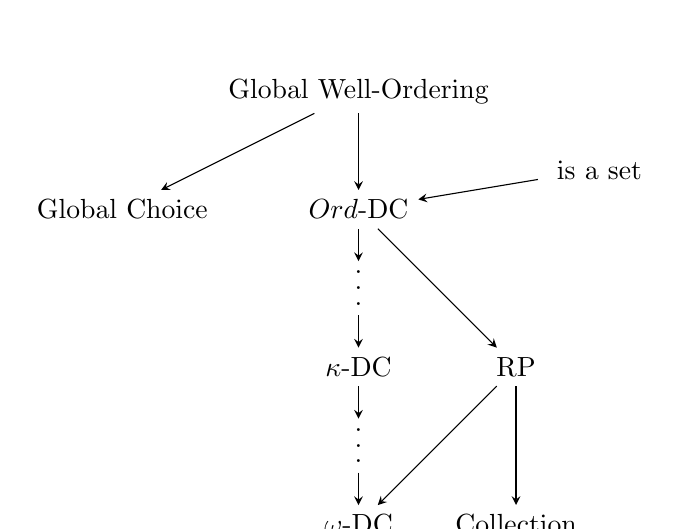
\begin{tikzpicture}
\begin{scope}[every node/.style={}]
    \node (A) at (8, -2.5) {Collection};
    \node (B) at (9, 2){$\A$ is a set};
    \node (C) at (3, 1.5){Global Choice};
    \node (D) at (6,1.5) {$Ord$-DC };
    \node (E) at (6, -0.5) {$\kappa$-DC};
    \node (I) at (8, -0.5) {RP};


    \node (L) at (6, 0.7) {.};
    \node (M) at (6, 0.5) {.};
    \node (N) at (6, 0.3) {.};
    \node (P) at (6, -1.7) {.};
    \node (Q) at (6, -1.5) {.};
    \node (R) at (6, -1.3) {.};
    \node (S) at (6, -2.5) {$\omega$-DC};
    \node (T) at (6, 3) {Global Well-Ordering};
    
\end{scope}

\begin{scope}[>={stealth},
              every node/.style={fill=white,circle},
              every edge/.style={draw=black}]

    \path [->] (T) edge (D);
\path [->] (T) edge (C);
     \path [->] (B) edge (D);
     


    \path [->] (I) edge (A);
      \path [->] (I) edge (S);
    \path [->] (D) edge (I);
    \path [->] (D) edge (L);
    \path [->] (N) edge (E);
    \path [->] (E) edge (R);
     \path [->] (P) edge (S);
       
\end{scope}
\end{tikzpicture}
 \caption{Implication diagram in $\GBUR$}
 \label{GBUdiagram}
\end{center}
\end{figure}
\FloatBarrier
\subsection{Interpreting $\mathcal{U}$ in $\mathcal{V}$}\label{section:interpretingUrelementsinClassTheory}
The construction of $V\llbracket X \rrbracket$ introduced in Section \ref{section:interpretingUinV} can be easily generalized to interpreting urelement class theory in pure class theory.
\begin{definition}\label{barwiseinterpretation2}
Let $\<V, \in , \mathscr{V}>$ be a model of GBc and $X \in \mathscr{V}$. $\<V \llbracket X \rrbracket, \bar{A}, \bar{\in}>$ is then defined as in Definition \ref{barwiseinterpretation1}. Let $\mathscr{V}\llbracket X \rrbracket = \{Y \in \mathscr{V} : Y \subseteq  V \llbracket X \rrbracket\}$. $\mathscr{V}\llbracket X \rrbracket$ denotes the model $\< V \llbracket X \rrbracket, \bar{A}, \bar{\in}, \mathscr{V}\llbracket X \rrbracket>$.\footnote{Note that when $Y \in \mathscr{V}\llbracket X \rrbracket$, $\mathscr{V}\llbracket X \rrbracket \models x \in Y$ if and only if $\mathscr{V} \models x \in Y$.}
\end{definition}

\begin{theorem}\label{Con(KM)->Con(KMU)}
Suppose $\mathscr{V} \models $ GBc and $X$ is a class in $\mathscr{V}$. Then
\begin{enumerate}
    \item $\mathscr{V}\llbracket X \rrbracket \models $ $\GBUR$ + Collection;
    \item $\mathscr{V}\llbracket X \rrbracket \models $ $\KMUR$ + Collection if $\mathcal{V} \models$ KMc;
    \item $\mathscr{V}\llbracket X \rrbracket \models $ CC if $\mathscr{V} \models$ CC;
    \item $\mathscr{V}\llbracket X \rrbracket \models $ Limitation of Size (and hence GBCU) if $\mathcal{V} \models$ GBC.
\end{enumerate}
\end{theorem}

\begin{proof}


For (1) and (2), $\mathscr{V}\llbracket X \rrbracket \models$ ZU by Theorem \ref{thm:V[X]modelsZFU}, so it remains to show that $\mathscr{V}\llbracket X \rrbracket$ satisfies Collection, Class Extensionality, and First-Order Comprehension (or Full Comprehension), all of which follow easily from the fact that $\mathscr{V} \models$ GBc (or KMc). For example, to show $\mathscr{V}\llbracket X \rrbracket \models$ Collection, suppose that in $\mathscr{V}\llbracket X \rrbracket$ for every $x \in \barw$ there is some $y$ such that $x \bar{R} y$ for some $\barw, \bar{R} \in \mathscr{V}\llbracket X \rrbracket$, where $\barw = \<1, w>$. Then in $V$ there is some $v \subseteq V \llbracket X \rrbracket$ such that for every $\barx \in w$, there is some $\bary \in v$ such that $\mathscr{V}\llbracket X \rrbracket \models \<\barx, \bary> \in \bar{R}$. Then $\bar{v} = \<1, v>$ is a desired collection set in $\mathscr{V}\llbracket X \rrbracket$.

(3) Suppose that $\mathscr{V} \models$ CC AND for every $\barx \in V\llbracket X \rrbracket$, there is some class $\bar{X} \in \mathscr{V}\llbracket X \rrbracket$ with $\varphi(\barx, \bar{X}, \bar{Z})^{ \mathscr{V}\llbracket X \rrbracket}$. By CC in $\mathscr{V}$, there is a class $Y \subseteq V\llbracket X \rrbracket \times U$ such that for every $\barx \in V\llbracket X \rrbracket$, $\varphi(\barx, Y_{\barx}, \bar{Z})^{ \mathscr{V}\llbracket X \rrbracket}$ and $Y_{\barx} $ is a class of $\mathscr{V}\llbracket X \rrbracket$. Define $\overline{Y} = \{\overline{\<\barx, \bary>} : \bary \in Y_{\barx} \land \barx \in \mathscr{V}\llbracket X \rrbracket \}$ (where $\overline{\<\barx, \bary>}$ codes the ordered-pair as in Theorem \ref{thm:ACholdsViffACholdsinV[X]}), which is a class of $\mathscr{V}\llbracket X \rrbracket$. Since for every $\barx \in \mathscr{V}\llbracket X \rrbracket$, $\mathscr{V}\llbracket X \rrbracket \models Y_{\barx} = \overline{Y}_{\barx}$, it follows that CC holds in $\mathscr{V}\llbracket X \rrbracket$.

(4) Suppose that $\mathscr{V}$ Global Well-Ordering. Note that if $\bar{Y}$ and $\bar{Z}$ are two proper classes in $\mathscr{V}\llbracket X \rrbracket$ , they must be equinumerous proper classes in $\mathscr{V}$ by Propostion \ref{prop:GC<->GWO<->LS}. So in $\mathscr{V}$ there must be a bijection $F$ between $\bar{Y}$ and $\bar{Z}$. Then $\bar{F} = \{ \overline{\<\bary, \barz>} : F(\bary) = \barz \}$ will be a bijection between $\bar{Y}$ and $\bar{Z}$ in $\mathscr{V}\llbracket X \rrbracket$.\end{proof}


\begin{theorem}\label{KMU+LSbiintepsKM+LS}
The following pairs of theories are bi-interpretable with parameters.
\begin{enumerate}
    \item GBC and GBCU + $\A \sim \omega$;
    \item KMC and KMCU + $\A \sim \omega$;
    \item GBC and GBCU + Limitation of Size;
    \item KMC and KMCU + Limitation of Size;
    \item GBC and GBCU + Limitation of Size + Plenitude;
    \item KMC and KMCU + Limitation of Size + Plenitude.
\end{enumerate}
\end{theorem}
\begin{proof}
Working in GBC (KMC), we can form either $\mathscr{V}\llbracket \omega \rrbracket$ (or $V\llbracket Ord\rrbracket$), and the map $y \mapsto \hat{y}$ and $Y \mapsto \hat{Y} = \{\hat{y} : y \in Y\}$ will be a definable isomorphism between $\mathcal{V}$ and $V^{\mathcal{V}\llbracket \omega \rrbracket}$ (or $V^{\mathcal{V}\llbracket Ord \rrbracket}$). In KMCU + Limitation of Size, there will be an injective map $F$ from $\A$ to $V$. For every urelement $a$, let $\tilde{a} = \<0, F(a)>$; and for every set $x$, we let $\tilde{x} = \<1, \{\tilde{y} : y \in x\}>$. It follows by an easy induction that the map $x \mapsto \tilde{x}$ and $X \mapsto \tilde{X} = \{\tilde{x} : x \in X\}$ is an isomorphism between $U$ and $V\llbracket F[\A] \rrbracket$.
\end{proof}

\begin{corollary}\label{corollary:LS<->AlessthanV}
Over KMCU, the following are equivalent.
\begin{enumerate}
    \item Limitation of Size.
    \item There is an injective map from $\A$ to $V$.
\end{enumerate}
\end{corollary}
\begin{proof}
(1) $\rightarrow$ (2) is clear. For (2) $\rightarrow$ (1), first observe that over KMCU, Limitation of Size holds for the pure classes $\mathcal{V}$. For, given a global choice function, its restriction to $V$ is a pure class so $\mathcal{V} \models $ Global Choice, which means $\mathcal{V} \models $ Limitation of Size by Proposition \ref{prop:GC<->GWO<->LS}. Now suppose that $F$ is an injective map from $\A$ to $V$. Since $U$ and $V\llbracket F[\A] \rrbracket$ are equinumerous, every proper class is equinumerous with a pure proper class. Therefore, all proper classes are equinumerous.
\end{proof}

\subsection{Independence results}\label{section:independenceinClassTheory}
In this subsection, I discuss several independence results concerning the completeness of Diagram \ref{GBUdiagram} over $\KMUR$. To begin with, arguments in \ref{subsection:implicationdiagram} which appeal to homogeneity can no longer go through in the context of class theory. For example, one might attempt to show that $\KMUR$ + Plenitude implies $\omega$-DC by the same argument as in Theorem \ref{Plenitude->DCS}. But the problem is that the ``kernel'' of a class relation $R$ might be a proper class, in which case we cannot find some a set of urelements that is big enough to ``fix'' $R$. In fact, we will see that over $\KMUR$,
\begin{enumerate}
    \item $\kappa$-DC $\nrightarrow$ Collection;
    \item Global Choice  $\nrightarrow$ ($\omega$-DC $\lor$ Collection);
    \item Collection $\nrightarrow$ $\omega$-DC;
    \item RP $\nrightarrow$ $\omega_1$-DC.
\end{enumerate}
Since it is well-known that KMc cannot prove Global Well-Ordering, it follows that Diagram \ref{GBUdiagram} is indeed complete over $\KMUR$.

Let me first discuss a general method of constructing \textit{class permutation models} of $\KMUR$ used in \cite{felgner1976choice}. Given a model $\<U, \A, \in, \U>$ of KMCU, we might fix an $\A$-ideal $\I$ as in Definition \ref{normalideal} and consider $U^\I$, the class of all first-order objects whose kernel is small in the sense of $\I$. This will give us a model of $\ZFCUR$ as before. To have a model of $\KMUR$, however, we cannot take all subclasses of $U^I$ as the second-order part of $U^\I$. To see this, suppose that $\A$ is an infinite set and $\I$ is its ideal of finite subsets; then an injection $F$ from $\omega$ to $\A$ will be a subclass of $U^\I$, which means having $F$ as a class of the model we intend to build would violate Replacement. In other words, we need to throw out some subclasses of $U^\I$. This is done by finding some suitable group $\G$ of permutations on $\A$ and only keep those subclasses of $U^\I$ that are \textit{symmetric} with respect to $\I$ and $\G$.

\begin{definition}[KMCU]
Let $\G$ be a group of permutations of $\A$.\footnote{It is understood that every $\pi \in \G$ is a permutation of a \textit{set} of urelements. Whenever $\pi, \sigma \in \G$, $\pi \circ \sigma$ is taken as the composition of their canonical extensions, which point-wise fix the urelements not in their original domains.} For any $x \in U$, $sym(x)$ and $fix(x)$ are defined as in Definition \ref{permutationmodeldef}. Let $\I\in \U$ be an $\A$-ideal as in Definition \ref{normalideal}. $\I$ is said to be $\G$-\textit{flexible} if 
\begin{enumerate}
    \item for every $\pi \in \G$ and $A \in \I$, $\pi A \in \I$;
    \item $\I$ has a \textit{basis} such that for every $B$ in the basis and $ A \in \I$ disjoint from $B$, there is some $\pi \in fix(B)$ such that $\pi A \neq A$.
\end{enumerate}
A class $X$ is \textit{symmetric} (w.r.t. $\G$ and $\I$) if there is some $A \in \I$, called a \textit{support} of $X$, such that $fix(A) \subseteq sym(X)$, where $sym(X) = \{\pi \in \G : \pi X = X\}$.  $U^\I =\{ x\in U : ker(x) \in \I\}$. $\W = \{ X \subseteq U^\I : X \text{ is symmetric}\}$. The model $\<U^\I, \in, \A, \W>$ is also denoted by $\W$.
\end{definition}
\noindent As we shall see later, $\G$-flexibility ensures that enough classes are thrown out so that Replacement can hold in $\W$. It is easy to check that every $\pi \in \G$ is an automorphism of $\W$ because $\I$ is $\G$-flexible.

\begin{theorem}[KMCU]\label{classpermutationmodel}
Let $\G$ be a group of permutations on $\A$ and $\I$ be an $\A$-ideal that is $\G$-flexible. Then $\W \models \KMUR$. 
\end{theorem}
\begin{proof}
$\W$ is a transitive class containing all the urelements and pure sets. And by the same argument as in Theorem \ref{smallkernelmodel}, it follows that $\W \models $ ZU + AC + Separation + Class Extensionality.  


To show $\W \models$ Replacement, suppose that $x \in \W$ be a set and $F \in \W$ be a class function on $x$ with a support $A \in \I$. Let $\mathcal{J}$ be a basis of $\I$ which witnesses its flexibility and $B$ be a set of urelements in $\J$ with $ker(x) \cup A \subseteq B$. It suffices to show that $ker(F[x]) \subseteq B$. If not, then there is some $y \in F[x]$ such that $ker(y) \setminus B$ is not empty. Since $ker(y) \setminus B \in \I$, it follows that there is some $\pi \in fix(B)$ such that $\pi (ker(y) \setminus B) \neq ker(y) \setminus B$, and as a result, $\pi y \neq y$. But $F(z) = y$ for some $z \in x$ so $F(z) = \pi y$, which is a contradiction.


To show that Full Comprehension holds in $\W$, fix a formula $\varphi$ in the language of urelement class theory and classes $X_0, .., X_n \in \W$, in $\U$ let $X = \{ x \in  \W: \W \models \varphi (x, X_0, ... ,X_n \}$. It suffices to show that $sym(X_0) \cap ... \cap sym(X_n) \subseteq Sym(X)$. Fix a $\pi \in sym(X_0) \cap ... \cap sym(X_n)$. For every $x \in X$, since $\pi$ is an automorphism of $\W$, it follows that $\W \models \varphi (\pi x, X_0, ..., X_n)$ and hence $\pi x \in X$. Therefore, $\pi X = X$.
\end{proof}
\begin{theorem}\label{thm:KMUR+kDCvdashCollection}
Assume the consistency of KM. Let $\kappa$ be any infinite cardinal. There is a model of $\KMUR$ in which
\begin{enumerate}
    \item $\kappa$-DC holds;
    \item Collection fails.
\end{enumerate}
\end{theorem}
\begin{proof}
Let $\U$ be a model of KMCU + $\A \sim \aleph_{\kappa^+}$. Let $\I$ be the ideal of all sets of urelements of size less than $\aleph_{\kappa^+}$ and $\G$ be the group of all permutations of $\A$. It is clear that $\I$ is $\G$-flexible, so the resultant model $\W$ satisfies $\KMUR$. Collection fails in $\W$ because every cardinal below $\aleph_{\kappa^+}$ is realized while $\aleph_{\kappa^+}$ is not. To show $\kappa$-DC holds in $\W$, suppose that $R$ is a class relation in $\W$ without terminal nodes. Since the first-order domain of $\W$, $U^\I$, is closed under $\kappa$-sequences, $\U$ thinks that $\forall s \in (U^\I)^{<\kappa} \exists y \in U^\I R(x, y)$; by $Ord$-DC in $\U$, it follows that there is an $f \in (U^\I)^{\kappa}$ such that $R(f\restriction \alpha, f(\alpha))$ for every $\alpha < \kappa$. $f$ lives in $U^\I$, so $\kappa$-DC holds in $\W$.
\end{proof}


\begin{theorem}[Felgner \cite{felgner1976choice}]\label{thm:KMURnvdashCollection}
Assume the consistency of KM. There is a model of $\KMUR$ in which
\begin{enumerate}
    \item Global Choice holds;
    \item $\omega$-DC fails;
    \item Collection fails.
\end{enumerate}
\end{theorem}
\begin{proof}
Let $\U$ be a model of KMCU + $\A \sim \omega$, in which we identify $\A$ with the rationals $\<\Q, <_\Q>$. Let $\G$ be the group of permutations of $\A$ that preserves $<_\Q$ and $\I$ be the ideal of finite subsets of $\A$. $\I$ is $\G$-flexible: if $A, B \in \I$ are disjoint, for any $b \in B \setminus A$, there is an open interval containing $b$ that is disjoint from $A \cup B \setminus \{b\}$; so we can permute this interval in an order-preserving way and leave $A$ point-wise fixed. By Theorem \ref{classpermutationmodel}, it follows that the resultant class permutation model $\W$ satisfies $\KMUR$. Moreover, both Collection and $\omega$-DC fail in $\W$ since there is a proper class of urelements but every set of them is only finite. For a proof of $\W \models$ Global Choice, see \cite[pp. 249-250]{felgner1976choice} or \cite[Lemma 2.3]{yao2022reflection}. \end{proof}

\begin{theorem}\label{kmudoesnotproveDC}
Assume the consistency of KM. There is a model of $\KMUR$ in which 
\begin{enumerate}
    \item Collection holds;
    \item Plenitude holds;
    \item $\omega$-DC fails.
\end{enumerate}
\end{theorem}

\begin{proof}
The model used here is also due to Felgner\cite{felgner1976choice}. The point here is that the model also satisfies Collection, which is not discussed in Felgner's paper. Let $\U$ be a model of KMCU with an enumeration of $\A$ with the tree $Ord^{<\omega}\setminus \{\emptyset\}$ consisting of all non-empty finite sequences of ordinals. Each urelement is identified with a node on the tree and define $a \lhd b$ as $a \subsetneq b$. $b$ is said to be an \textit{immediate descendant} of $a$ if $b$ extends $a$ by one digit. $b$ and $b'$ are \textit{siblings} if either they are both top nodes, or they are an immediate descendant of the same node. A set $t \subseteq \A$ is a \textit{tree} if it is closed under initial segment (i.e, if $b \in t$ and $a \lhd b$, then $a \in t$). A \textit{path} of a tree $t$ with length $\alpha$ is a function $f: \alpha \rightarrow Ord$ such that $f\restriction \beta \in t$ for all $\beta < \alpha$. A \textit{branch} is a maximal path, i.e., it is not properly extended by any path of the tree. A tree $t$ is \textit{small} if it has no infinite branch. Let $\T$ be the class of all small trees, which forms a basis for an ideal $\I$. Let $\G$ be the group of  permutations of $\A$ that preserves $\lhd$.
\begin{lemma}\label{treeflexible}
$\I$ is $\G$-flexible with respect to the basis $\T$.
\end{lemma}
\begin{proof}
If $a$ and $b$ are siblings with domain $n + 1$, then there is a natural permutation $\pi^a_b \in \G$ such that for every node $c$ with $dom(c) = j +1$ and $i < j+1$,
\begin{equation*}
   \pi^a_b c (i)  =
    \begin{cases*}
      b(n) & if $i = n$, $c(n) = a(n)$ and $c \restriction n = a \restriction n$  \\
      a(n) & if $i = n$, $c(n) = b(n)$ and $c \restriction n = a \restriction n$  \\
      c(i) & otherwise
    \end{cases*}
 \end{equation*}
 $\pi^a_b$ thus swaps only $a$ and $b$ and their descendants. Given a small tree $t$ and some $A \in \I$ disjoint from $t$, since every node has  $Ord$-many siblings we can find a node $a$ in $A$ and a sibling $b$ of $a$ such that $b \notin t \cup A$. $\pi^a_b$ will then leave $t$ point-wise fixed because $t$ is a tree.
\end{proof}
\noindent Therefore, the class permutation model $\W$ given by $\G$ and $\I$ satisfies $\KMUR$. $\W$ clearly satisfies Plenitude because for every $\kappa$, there are $\kappa$-many top nodes on the tree $Ord^{<\omega}\setminus \{\emptyset\}$. Suppose \textit{for reductio} that $\omega$-DC holds in $\W$. Since in $\W$ every $a \in \A $ has some $b \in A$ such that $a \lhd b$, then in $\W$ there is an infinite branch $s = \<a_n : n < \omega>$ such that $a_n \lhd a_{n+1}$ for every $n$. Let $t$ be a small tree such that $fix(t) \subseteq sym(s)$. Fix some $a_n$ not in $t$ and some sibling $b$ of $a_n$ such that $b \notin t$. Then $\pi_{a_n, b} \in fix(t)$ but $\pi_{a_n, b} (s) \neq s$, which is a contradiction.

It remains to show that $\W \models$ Collection. For any two small tress $t$ and $t'$, we say that $t$ \textit{mildly extend} $t'$ if $t' \subseteq t$ and no branch of $t$ properly extends a branch of $t'$.


\begin{lemma}\label{treelemma}
Let $t_0, t_1 \in \T$ be such that $t_0 \subseteq t_1$ and every terminal node in $t_0$ has a descendent in $t_1$. Then for every $t \in \T$, there is a $\pi \in fix(t_0)$ such that $ t_1 \cup \pi t $ mildly extends $t_1$.  
\end{lemma}
\begin{proof}
Define $M = \{ a \in t_1 \setminus t_0 : a \text{ is an initial node in } t_1 \setminus t_0 \text{ and } a \text{ has a descendant in } t\}$, where ``$a$ initial in $t_1 \setminus t_0$'' means there is no node $b \in t_1 \setminus t_0$ such that $b \lhd a$. Since every node has $Ord$-many siblings and Global Well-Ordering holds in $\U$, for every $a \in M$ we can pick a sibling $a'$ of $a$ such that $a' \notin t_1 \cup t$, and we can ensure that $a_1' \neq a_2'$ for any distinct  $a_1, a_2 \in M$. Let $\pi = \bigcup_{a \in M}\pi^a_{a'}$, which is in $\G$. $\pi \in fix(t_0)$, because no node in $t_0$ is a descendant of any node in $M$ and $\pi$ only moves nodes in $M$ and their descendants.

To show that $t_1 \cup \pi t $ mildly extends $t_1$, consider any branch $f$ of $t_1$. Suppose \textit{for reductio} that $f$ is properly extended by a branch $g$ of $\pi t$. Note that $f$ must contain a node not in $t_0$ since otherwise $f$ would be a branch of $t_0$, which is impossible because every branch of $t_0$ is properly extended by a branch of $t_1$. So let $a$ be the least such node. There is a node $b$ on $g$ such that $a \lhd b$, where $b =\pi c$ for some $c \in t$. It follows that $a$ must be in $M$. If not, then $\pi a = a$ so $a \lhd c$ and hence $a$ is in $M$ after all. Thus, $\pi a = a'$ for some $a' \notin t$, but then $a' \lhd c$ so $a' \in t$---contradiction.
\end{proof}

\begin{lemma}
For any infinite cardinal $\kappa$, if $\<t_\alpha : \alpha < \kappa>$ is a sequence of small trees such that $t_\alpha$ mildly extends $\bigcup_{\beta < \alpha} t_\beta$ for every $\alpha < \kappa$, then $\bigcup_{\alpha < \kappa} t_\alpha$ is a small tree.
\end{lemma}
\begin{proof}
Let $t= \bigcup_{\alpha < \kappa} t_\alpha$. Suppose \textit{for reductio} that $f$ is an infinite branch of $t$. There will be some $t_\alpha$ with some $0 < m < \omega$ such that $f\restriction m$ is a branch of $t_\alpha$. Then for some $\beta > \alpha$, $t_\beta$ contains a branch that extends $f \restriction m$, which contradicts the assumption.
\end{proof}

Now suppose that $\W \models \forall x \in w \exists y \<x, y> \in R$ for some $w, R \in \W$. Let $t_0$ be a small tree that includes $ker(w)$ and some support of $R$, and enumerate $w$ by $\{x_\alpha : \alpha <\kappa\}$ for some $\kappa$. In $U$, we define a $\kappa$-sequence of small tress $\<t_\alpha : \alpha < \kappa>$ such that 
\begin{itemize}
    \item [] (i) $t_\alpha$ mildly extends $\bigcup_{\beta < \alpha} t_\beta$ for every $\alpha < \kappa$;
    \item [] (ii) for each $x_\alpha$, there is some $y \in \W$ such that $\<x_\alpha, y> \in R$ and $ker(y) \subseteq  t_\alpha$.
\end{itemize}
This is possible, because for every $x_\alpha$, fix some $y'$ with $\<x, y'> \in R$. Since $ker(y')$ is a subset of some small tree $t$, by Lemma \ref{treelemma}, there is a $\pi \in fix (t_0)$ such that $\bigcup_{\beta < \alpha} t_\beta \cup \pi t$ mildly extends $\bigcup_{\beta < \alpha} t_\beta$. Thus $\<x_\alpha, \pi y'> \in R$ and $ker(\pi y') \subseteq \pi t$. Let $t_\kappa = \bigcup_{\alpha < \kappa} t_\alpha$, which is a small tree. It follows that $\forall x \in w \exists y \in V(t_\kappa) \ (\<x, y> \in R)$, which suffices for Collection in $\W$.
\end{proof}
\noindent By using the same argument at the previous theorem, it is not hard to show that $\W \models \kappa$-CC for every infinite cardinal $\kappa$. However, it is unclear if the model $\W$ in Theorem \ref{kmudoesnotproveDC} satisfies CC if we assume $\U \models$ CC. 


\begin{theorem}\label{thm:RPnvdashOmega1Dc}
Assume the consistency of KM. There is a model of $\KMUR$ in which 
\begin{enumerate}
    \item RP holds;
    \item Plenitude holds;
    \item $\omega_1$-DC fails.
\end{enumerate}
\end{theorem}
\begin{proof}
Let $\U$ be a model of KMCU with an enumeration of $\A$ with the tree $Ord^{<{\omega_1}}\setminus \{\emptyset\}$ consisting of all non-empty \textit{countable} sequences of ordinals. A set $t$ of urelements is an $\omega_1$-small tree if it is a tree without any $\omega_1$-branch. Let $\I$ be the ideal generated by all the $\omega_1$-small trees and $\G$ be the group of permutations of $\A$ that preserve the tree structure as in the proof of Theorem \ref{kmudoesnotproveDC}. Since the same arguments in Lemma \ref{treeflexible} and \ref{treelemma} still go through, it follows that $\I$ is $\G$-flexible and that Collection holds in the resultant model $\W$.
\begin{claim}
$\W \models $ RP. 
\end{claim}
\begin{claimproof}
By Proposition \ref{prop:rp+gbur<->collection+dcs}, it is enough to show that $\omega$-DC holds in $\W$. So it suffices to show that the ideal $\I$ is countably closed. This is simply because the union countably many $\omega_1$-small trees, $\{t_n : n< \omega \}$, is an $\omega_1$-small tree. 
\end{claimproof}
\begin{claim}
$\W \models $ $\neg$($\omega_1$-DC).
\end{claim}
\begin{claimproof}
Suppose \textit{for reductio} that $\omega_1$-DC holds in $\W$. Say that a sequence $s \in \A^\alpha$ is a \textit{chain} if $s(\beta) \lhd s(\beta')$ for every $\beta < \beta' < \alpha$; and $s$ is said to be \textit{bound} by $a$ if $s(\beta) \lhd a$ for every $\beta < a$. In $\W$, every chain $s\in \A^{<\omega_1}$ has a bound $a \in \A$. By  $\omega_1$-DC, in $\W$ there is an $f \in \A^{\omega_1}$ that is a chain of length $\omega_1$. Then $ker(f)$ must be contained in some $\omega_1$-small tree, which is impossible.
\end{claimproof}

\end{proof}

\subsection{Open questions}
It is a classic result that GBC is a conservative extension of ZFC (e.g., see \cite{felgner1976choice}). But we know that GBCU is \textit{not} a conservative extension of ZFCU: GBCU proves that either $\A$ is a set, or Plenititude holds, which is not provable in ZFCU.
\begin{question}
\
\begin{enumerate}
    \item Is $\GBUR$ + Global Choice conservative over $\ZFCUR$?
    \item Is $\GBUR$ + Collection + Global Choice conservative over ZFCU?
\end{enumerate}
\end{question} 
\noindent Given Theorem \ref{kmudoesnotproveDC} and the fact that CC is a stronger version of Collection, it is natural to ask the following.
\begin{question}
Does $\KMUR$ prove any of the following?
\begin{enumerate}
    \item Collection $\land$ Global Choice $\rightarrow$ $\omega$-DC.
    \item CC $\rightarrow$ $\omega$-DC.
    \item CC $\land$ Global Choice $\rightarrow$ $\omega$-DC.
\end{enumerate}
\end{question}
A natural question arises at this point as in Section \ref{section:WhatisZFCU}: what is KMc (or, GBc) class theory with urelements if we only wish to have AC for sets? Notably, in both class and set theory with urelements, Collection tends to lose its strength without enough choice. As previously conjectured, $\ZFUR$ + Collection does not prove RP, and in fact, $\ZFUR$ + DC should not be able to prove the DC$_\omega$-scheme. Theorem \ref{kmudoesnotproveDC} confirms that this is indeed the case in urelement class theory. Thus, although Collection is still strictly stronger than Replacement in class theory with urelements, adding it into $\KMUR$ cannot produce a theory with sufficient strength. So perhaps a robust version of KMc with urelements \textit{should} include RP as an axiom since it implies $\omega$-DC (Proposition \ref{prop:rp+gbur<->collection+dcs}). However, RP cannot exclude \textit{all} pathological models: in the proof of Theorem \ref{thm:RPnvdashOmega1Dc}, the model satisfies RP but contains a $Ord$-splitting tree without any $\omega_1$-branch. That said, it seems that bringing urelements back to the picture inevitably invites \textit{axiomatic freedom}.





\section{Second-order reflection with urelements}\label{section:RP2withurelements}

\subsection{Bi-interpretabtion with few urelements}
The second-order reflection principle (first introduced by Bernays \cite{bernays1976problem}) is the  scheme

\begin{itemize}
    \item [] (RP$_2$) $\forall X [\varphi(X) \rightarrow \exists t( t \text{ is transitive} \land \varphi^t(X \cap t))]$,
\end{itemize}
where $\varphi$ can be any formula in the language of class theory, and $\varphi^t$ is the result of restricting all the first-order quantifiers to the members of $t$ and all the second-order quantifiers to the subsets of $t$. Thus, $\varphi^t(X \cap t)$ is simply the assertion $\<t, \in, P(t)> \models \varphi(X \cap t)$. As observed in \cite{bernays1976problem} and \cite{tait2005constructing}, RP$_2$ is able to ``bootstrap''. For example, with the Axiom of Separation, Foundation and Extensionality, RP$_2$ can recover the remaining axioms of KMC.

\begin{prop}
RP$_2$ + Separation + Extensionality + AC + Foundation $\vdash$ KMCU + CC. 
\end{prop}
\begin{proof}
Note that RP alone implies that every $x_1, ..., x_n$ will be contained in some transitive set since we can reflect the formula $\exists y (x_1 = y) \land ... \land \exists y (x_n =y)$. This implies Pairing and Union given Separation. Then we can reflect the assertion ''for every $x$,  $x \cup \{x\}$ exists" down to a transitive set to get Infinity. Collection (and hence Replacement) follows by Proposition \ref{prop:rp+gbur<->collection+dcs}. To get Powerset, note that for every set $u$, by Separation we have ``for every class $X$ that is a subclass of $u$, there is a set $x$ that is co-extensional with $X$''. So by RP$_2$ we can reflect this assertion down to some transitive set $t$ containing $u$. Accordingly, $t$ contains every subset of $u$ as a member, which suffices for Powerset given Separation.

For Class Choice, suppose \textit{for reductio} that $\forall x \exists X \varphi(x, X, Z)$ for some class $Z$ but there is no $Y \subseteq U \times U$ such that $\varphi(x, Y_x, Z)$. By RP$_2$, there is some transitive set $t$ such that $\forall x \in t \exists X \subseteq t \varphi^t(x, X, Z \cap t)$ and there is no $Y \subseteq t\times t$ such that $\forall x \in t \varphi^t (x, Y_x, Z \cap t)$. Since there is a well-ordering of $P(t)$, for every $x \in t$ we can choose a $y_x \in P(t)$ such that $\varphi^t(x, y_x, Z\cap t)$. Let $Y = \bigcup_{x \in t}\{\<x, z> : z \in y_x\}$. It follows that $\forall x \in t \varphi^t (x, Y_x, Z \cap t)$, which is a contradiction.

Similarly, to show that there is a global well-ordering, we suppose \textit{for reductio} that there is no global well-ordering and reflect this statement to some transitive set $t$ that is closed under pairs. Since there is a well-ordering of $t$, the reflected statement will yield a contradiction.

Finally, we also get Full Comprehension. This is because if there is a failure of Full Comprehension of the form $\neg \exists X \forall z (z \in X \leftrightarrow \varphi(x, P))$, then we can reflect it down to some transitive $t$ to get $\neg \exists x \subseteq t \forall z (z \in x \leftrightarrow \varphi^t(x, P \cap t))$, which will then contradict Separation.\footnote{As a consequence, note that RP$_2$ is equivalent to the following scheme, which asserts that every statement, possibly with class parameters, is absolute to some transitive set.
\begin{itemize}
    \item [] (RP$_2^+$) $\forall X \exists \text{ transitive } t (\varphi(X) \leftrightarrow \varphi^t(X \cap t))$.
\end{itemize}
This is because given $\varphi$ and some class $X$, by Full Comprehension we can form the class $Y$ such that $\forall y (y \in Y \leftrightarrow \varphi(X))$; then by RP$_2$, there will be a non-empty transitive set $t$ such that $\forall y \in t (y\in Y\cap t \leftrightarrow \varphi^t(X \cap t))$. It follows that $\varphi(X) \leftrightarrow \varphi^t (X \cap t)$.}\end{proof}

In pure class theory, the bootstrapping of RP$_2$ goes beyond KMC as it yields large cardinals. In particular, RP$_2$ implies the exsitence of a proper class of inaccessible cardinals, Mahlo cardinals and weakly compact cardinals (see \cite{tait2005constructing} for more on this). However, the consistency strength of RP$_2$ is bounded by ZFC + an $\omega$-Erd{\"o}s cardinal (see \cite[Exercise 9.18]{kanamori2008higher}), which is consistent with $V = L$. Some natural question arise in the context of urelements: What is the consistency strength of RP$_2$ in urelement class theory? Could it be somehow affected by urelements? 

The next lemma shows that the $\mathcal{V} \llbracket X \rrbracket$ construction introduced in Definition \ref{barwiseinterpretation2} preserves second-order reflection.
\begin{lemma}\label{lemma:KM+RP2interpretsKMU+RP2}
Let $\mathcal{V} \models$ KM + RP$_2$ and $W \in \mathcal{V}$ be a class. Then $\mathcal{V} \llbracket W \rrbracket \models $ KMU + RP$_2$ + Limitation of Size.
\end{lemma}
\begin{proof}
Since RP$_2$ + KM proves that there is a global well-ordering, which implies Limitation of Size over KM, by Theorem \ref{Con(KM)->Con(KMU)} it follows that $\mathcal{V} \llbracket W \rrbracket \models $ KMU + Limitation of Size. So it remains to show that every instance of RP$_2$ holds in $\mathcal{V} \llbracket W \rrbracket$. For every transitive set $t \in V$, let $t\llbracket W \rrbracket = \<1, V\llbracket W \rrbracket \cap t>$, which is a transitive set in $V\llbracket W \rrbracket$.

\begin{claim}\label{permu}
Let $t$ be a transitive set in $\mathcal{V}$. Then for any $x_1, ... x_n \in t\llbracket W \rrbracket$ and $X_1, ... ,X_m \in \mathcal{V} \llbracket W \rrbracket$, $ \mathcal{V} \models (\varphi^{\mathcal{V} \llbracket W \rrbracket})^t \leftrightarrow (\varphi^{t\llbracket W \rrbracket})^{\mathcal{V} \llbracket W \rrbracket}$ for any suitable formula $\varphi$ in the language of urelement class theory.
\end{claim}
\begin{claimproof}
If $\varphi$ is an atomic formula, then the claim holds because the definition of $\bar{\in}$ and $\bar{\A}$ (see Definition \ref{barwiseinterpretation1}) is absolute for transitive sets. Boolean cases commute. And if $\varphi$ is $\exists x \psi$, we have
\begin{align*}
    (\varphi^{\mathcal{V} \llbracket W \rrbracket})^t  &= (\exists x \in \mathcal{V} \llbracket W \rrbracket  \psi^{\mathcal{V} \llbracket W \rrbracket})^t \\
                &\Leftrightarrow \exists x \bar{\in} t\llbracket W \rrbracket (\psi^{\mathcal{V} \llbracket W \rrbracket})^t \\
                & \Leftrightarrow \exists x \bar{\in} t\llbracket W \rrbracket (\psi^{t\llbracket W \rrbracket})^{\mathcal{V} \llbracket W \rrbracket} \tag*{(by induction hypothesis)} \\
                & = (\varphi^{t\llbracket W \rrbracket})^{\mathcal{V} \llbracket W \rrbracket}.
\end{align*}
Similarly, if $\varphi$ is $\exists X \psi$, then we have
\begin{align*}
    (\varphi^{\mathcal{V} \llbracket W \rrbracket})^t  &= (\exists X \subseteq V \llbracket W \rrbracket  \psi^{\mathcal{V} \llbracket W \rrbracket})^t \\
                &\Leftrightarrow \exists X \subseteq t\llbracket W \rrbracket (\psi^{\mathcal{V} \llbracket W \rrbracket})^t \\
                & \Leftrightarrow \exists  X \subseteq t\llbracket W \rrbracket (\psi^{t\llbracket W \rrbracket})^{\mathcal{V} \llbracket W \rrbracket} \tag*{(by induction hypothesis)}\\
                & = (\varphi^{t\llbracket W \rrbracket})^{\mathcal{V} \llbracket W \rrbracket}.
\end{align*}
This proves the claim.                                                  \end{claimproof}

Now if $\mathcal{V} \llbracket W \rrbracket \models \varphi$, then we can reflect $\varphi^{\mathcal{V} \llbracket W \rrbracket}$ in $\mathcal{V}$ down to some transitive set $t$. By the claim, it follows that $\mathcal{V} \llbracket W \rrbracket \models \varphi ^{t\llbracket W \rrbracket}$. Hence, $\mathcal{V} \llbracket W \rrbracket \models$ RP$_2$. \end{proof}
\begin{theorem}\label{KM + RP <-> KMU + RP + LS}
KM + RP$_2$ and KMU + RP$_2$ + Limitation of Size are bi-interpretable with parameters. \qed
\end{theorem}
\begin{proof}
First note that KMU + RP$_2$ also interprets KM + RP$_2$, because if $\mathcal{U} \models$ KMU + RP$_2$, then its pure part $\mathcal{V} \models$ KM + RP$_2$. For, as in Lemma \ref{lemma:KM+RP2interpretsKMU+RP2}, given a transitive $t \in U$, we can show that $(\varphi^{\mathcal{V}})^t \leftrightarrow (\varphi^{V\cap t})^\mathcal{V}$, where $V\cap t$ is a transitive pure set. So if $\mathcal{V} \models \varphi$, then we can reflect $\varphi^\mathcal{V}$ to some transitive set $t$, which implies $\mathcal{V} \models \varphi^{V\cap t}$. And given Lemma \ref{lemma:KM+RP2interpretsKMU+RP2}, it follows that KM + RP$_2$ and KMU + RP$_2$ + Limitation of Size are mutually interpretable. And their bi-interpretability (with parameters) follows from Theorem \ref{KMU+LSbiintepsKM+LS}.
\end{proof}
 As a consequence, KMU + RP$_2$ also implies the existence of a proper class of inaccessible cardinals, Mahlo cardinals and weakly compact cardinals. By Corollary \ref{corollary:LS<->AlessthanV}, it follows that when the urelements are \textit{few}, i.e., no more numerous than the pure sets, RP$_2$ has the same strength as in pure class theory.


\subsection{A model of RP$_2$ with many urelements}\label{section:amodelofKMU+RP2+notLS}
What if there are more urelements than the pure sets? Or, does KMU + RP$_2$ prove Limitation of Size? In this final section, I construct a model of KMU + RP$_2$ where the urelements are more numerous than the pure sets by assuming the consistency of a $\kappa^+$-supercompact cardinal. To begin with, there is an alternative accumulative hierarchy that can produce natural models of KMCU where Limitation of Size fails.
\begin{definition}
Let  $\kappa$ be an infinite cardinal. For any set $x$, $P_\kappa(x)$ is the set of all subsets of $x$ of size less than $\kappa$. For any set of urelements $A$, $U_{\kappa, A} = \bigcup_{B \in P_\kappa (A)} V_\kappa (B)$. $\mathcal{U}_{\kappa, A}$ denotes the model $\langle U_{\kappa, A}, A, \in, P(U_{\kappa, A})\rangle$ .
\end{definition}
\noindent The $U_{\kappa, A}$-hierarchy is a generalization of the $V_\kappa(A)$-hierarchy: $U_{\kappa, A} = V_\kappa(A)$ when the size of $A$ is no greater than $\kappa$. While every $A$ appeas as a set in $V_\kappa(A)$, $A$ would be a proper class in $U_{\kappa, A}$ when its size is greater than $\kappa$.  Another useful stratification is the $H_\kappa(A)$-hierarchy (used in \cite{HamkinsForthcoming-HAMRIS}), where $H_\kappa(A) = \{x \in U : ker(x) \subseteq A \land |trc(\{x\})| < \kappa \}$. Note that when $\kappa$ is inaccessible and $|A| > \kappa$, $H_\kappa(A) = U_{\kappa, A}$.
\begin{lemma}[ZFCU]\label{UKA}
For any transitive set $t$, the following are equivalent.
\begin{enumerate}
    \item $t = U_{\kappa, A}$, where $\kappa$ is inaccessible and $A \subseteq \A$ .
    \item $\<t, ker(t), \in, P(t)> \models$ $\KMUR$.
\end{enumerate}
In fact, $\mathcal{U}_{\kappa, A} \models $ KMCU + CC whenever $\kappa$ is inaccessible; and Limitation of Size fails in $\mathcal{U}_{\kappa, A}$ when $A$ has size greater than $\kappa$.
\end{lemma}
\begin{proof}
(1) $\rightarrow$ (2). $\mathcal{U}_{\kappa, A}\models$ ZU + Class Extensionality since it is transitive and sufficiently tall. For example, to show $\mathcal{U}_{\kappa, A}\models$ Powerset, fix some $x \in V_\alpha(B)$ for some $B \in P_\kappa(A)$ and $\alpha < \kappa$. Then $|V_\alpha(B)| < \kappa$ since $\kappa$ is a strong limit; so $P(x)$ is a subset of $V_\kappa(B)$ of size less than $\kappa$, and it will be contained in $V_\beta(B)$ for some $\beta <\kappa$ as $\kappa$ is regular. $\mathcal{U}_{\kappa, A}\models$ Global Well-Ordering since the well-ordering of  $U_{\kappa, A}$ in $U$ is a class of $U_{\kappa, A}$. To show $\mathcal{U}_{\kappa, A}\models$ Class Choice, suppose that $\mathcal{U}_{\kappa, A}\models \forall i \in I \exists X \varphi(i, X)$ for some $I \subseteq U_{\kappa, A}$. In $U$, we can well order $P(U_{\kappa, A})$ and then for each $i \in I$, choose some $X_i \in P(U_{\kappa, A})$ such that $\mathcal{U}_{\kappa, A}\models  \varphi(i, X_i)$. $Y = \bigcup_{i \in I}\{\<i, x> : x \in X_i\}$ will then be a desired class of $U_{\kappa, A}$. Note that Class Choice implies Collection and hence Replacement, so $\mathcal{U}_{\kappa, A}\models$ KMCU. And clearly, when $A$ has size greater than $\kappa$, $A$ and $\kappa$ are two proper classes in $\mathcal{U}_{\kappa, A}$ that are not equinumerous.

(2) $\rightarrow$ (1). Suppose that $ \mathcal{T} = \<t, ker(t), \in P(t)> \models$ $\KMUR$. Let $\kappa = Ord \cap t$. $\kappa$ must be a regular cardinal. Suppose not. Then given a cofinal sequence $f$ on $\kappa$ with length $\alpha$, where $\alpha < \kappa$, since $t$ is closed under ordered-pairs $f$ is a class function in $\mathcal{T}$ on $\alpha$. By Replacement in $\mathcal{T}$, it follows that $\kappa \in t$, which is a contradiction. To show $\kappa$ is a strong limit. First note that for every set $x \in t$, $P(x) = P^\mathcal{T}(x)$. This is because for every set $y \subseteq x$, $y$ is a class in $\mathcal{T}$ and so by Separation in $\mathcal{T}$, $y \cap x = y \in t$. So if $\alpha < \kappa$, then $P(\alpha)$ is in $t$ and by AC in $\mathcal{T}$, it is equinumerous with some $\beta < \kappa$. Clearly, $\omega < \kappa$, so $\kappa$ is inaccessible. 


Now let $A = ker(t)$. It remains to show that $t = U_{\kappa, A}$. First note that $P_\kappa(t) \subseteq t$. For, any enumeration of $x$ with some ordinal $\alpha < \kappa$ is a class in $\mathcal{T}$, so $x \in t$ by Replacement in $\mathcal{T}$. If $B \subseteq A$ is of size less than $\kappa$, then by an easy induction $V_\alpha(B)$ has size less than $\kappa$ for all $\alpha < \kappa$. This shows that $U_{\kappa, A} \subseteq t$. For every set $x \in t$, let $B = ker(x)$. Since $\mathcal{T} \models \KMUR$, $B \in t$. Then $B$ must have size less than $\kappa$ because $\mathcal{T} \models B \sim \alpha$ for some $\alpha < \kappa$. Let $\beta$ be the least ordinal such that $x \in V_\beta(B)$. As $x \in t$, it is clear that $\beta < \kappa$. Therefore, $x \in U_{\kappa, A}$. This shows that $t = U_{\kappa, A}$.                                      
\end{proof}
 
 
 Recall Zermelo's Quasi-Categoricity Theorem: any full second-order model of second-order ZF is isomorphic to some $V_\kappa$, where $\kappa$ is inaccessible. Now let ZFCU$_2$ be the corresponding version of ZFCU formulated in the second-order language. We then have the following generalized quasi-categoricity theorem in ZFCU + Plenitude.

\begin{theorem}[ZFCU + Plenitude]
For every full second-order structure $\M$, $\M \models$ ZFCU$_2$ if and only if $\M$ is isomorphic to some $\mathcal{U}_{\kappa, A}$, where $A \subseteq \A$ and $\kappa$ is an inaccesible cardinal.
\end{theorem}
\begin{proof}
Since $\M \models$ ZFCU$_2$ and it is a full second-order model, a standard argument shows that $\in^\M$ is well-founded. By AC and Plenitude, we can then fix a bijection $i$ from $\A^\M$, the class of urelements in $\M$, to a set of urelements $A$. $i$ can then be extended to $\M$ by letting $i (x) = \{i(y) : y \ \in^\M x\}$ as in Mostowski collapse. $i[\M]$ is then a transitive set $t$ such that $\<t, ker(t), \in, P(t)> \models \KMUR$. So $t = U_{\kappa, A}$ for some $A \subseteq \A$ and inaccessible cardinal $\kappa$ by Lemma \ref{UKA}.
\end{proof}
Now I proceed to prove the following.
\begin{theorem}\label{thm:RP2nvdashLS}
Assume the consistency of  $\text{ZFC} + \exists \kappa (\kappa \text{ is } \kappa^+ \text{-supercompact})$. There is a model of KMCU in which
\begin{enumerate}
    \item RP$_2$ holds;
    \item Limitation of Size fails.
\end{enumerate}
\end{theorem}
\begin{proof}
Let $V \models \text{ZFC} + \exists \kappa (\kappa \text{ is } \kappa^+ \text{-supercompact})$, where $\kappa^+$-supercompactness is defined as having a normal fine measure on $P_{\kappa}(\kappa^+)$. Note that by class forcing we can add a global well-ordering to $V$ without adding any new sets, which yields a model $\mathcal{V} \models$ GBC + Limitation of Size +  $\exists \kappa (\kappa \text{ is } \kappa^+ \text{-supercompact})$. By Theorem \ref{Con(KM)->Con(KMU)}, this gives us a model $\U \models$ GBCU + Limitation of Size + Plenitude + $\exists \kappa (\kappa \text{ is } \kappa^+ \text{-supercompact})$ (e.g., consider $\<V\llbracket Ord\rrbracket, \{0\}\times Ord, \in, \mathcal{V}\llbracket Ord \rrbracket >$). Working in $\mathcal{U}$, let $F$ be a normal fine measure on $P_{\kappa}(\kappa^+)$. For any functions $f$ and $g$ on $P_{\kappa}(\kappa^+)$,  define the equivalence relation
$$f =_F g \text{ if and only if } \{ x \in P_{\kappa}(\kappa^+) : f(x) = g(x) \} \in F.$$ 
Global Well-Ordering then allows us to pick a unique $f$ from each equivalence class $[g]_{=_F}$ and then form an internal ultrapower $U/F$ as in the beginning of Section \ref{section:WhatisZFCU}, which is a class in $\U$. Note that since the first-order part $U$ satisfies ZFCU (in particular, Collection), \L{}o\'s's Theorem holds for $U/F$ (see Theorem \ref{thm:collection<->losthm}). That is, for every $f_1, ... f_n \in U/F$, $ U/F \models \varphi (f_1..., f_n)$ if and only if $\{x \in P_{\kappa}(\kappa^+): \varphi (f_1(x)...,f_n(x))\} \in F$. 

\begin{lemma}
$\in_F$ is a well-founded and set-like relation on $U/F$.
\end{lemma}
\begin{proof}
$\in_F$ is well-founded because $F$ is $\kappa$-complete. To show it is set-like, fix any $f \in U/F$ and let $X = \{g \in U/F : g \in_F f \}$. We may assume that the set $ \bar{y}= \{x \in P_{\kappa}(\kappa^+) : f(x) \neq \emptyset \}$ is in $F$. Let $\bar{z}$ be the set of all functions from $\bar{y}$ to $(\bigcup f[\bary]) \cup \{\emptyset\}$. For each $g \in_F f$, we define a function $g'$ on $P_{\kappa}(\kappa^+)$ as follows.
\begin{equation*}
    g' (x) =
    \begin{cases*}
      g(x) & if $g(x) \in f(x)$ \\
     \emptyset        & otherwise 
    \end{cases*}
  \end{equation*}
$g' \restriction \bary$ is in $\barz$ for every $g$ such that $g \in_F f$. It suffices to show that the map $g \mapsto g' \restriction \bary$ is 1-1 from $X$ into $\barz$. Consider two $g_1, g_2 \in X$ .  Since $\bary \cap \{x \in P_{\kappa}(\kappa^+) : g_1(x) \neq g_2(x) \land g_1(x) \in f(x) \land g_2(x) \in f(x)\}$ is in $F$, there must be some $x \in \bary$ such that $g_1'(x) \neq g_2'(x)$ and hence $g_1' \restriction \bary \neq g_2' \restriction \bary$.
\end{proof}

Now we wish to collapse $U/F$ into a transitive class $M$, which yields an elementary embedding from $U$ to $M$. For reasons that will be clear, it is useful to have the elementary embedding fix $\kappa^+$-many urelements.\footnote{Note that we cannot expect the resulting elementary embedding $j$ to fix all the urelements. Otherwise, let $A$ be a set of urelements of size $\kappa$; then $j(A) = A$ but $|j(A)| = j(\kappa) > \kappa $.} So let $A$ be a set of urelements in $U$ enumerated by $\langle a_\alpha : \alpha < \kappa^+\rangle$. For every $y \in U$, let $C_y \in U/F$ be the function that is $=_F$-equivalent to the constant function that maps everything to $y$. Since all proper classes are equinumerous in $\mathcal{U}$, there is a one-one mapping $G$ from $\A_F \setminus \{C_{a_\alpha}: \alpha < \kappa^+ \}$ into $\A \setminus A$, where $\A_F$ is the class of urelements in $U/F$. We then define the collapsing function $\pi$ as follows. For every $f \in \A_F$, 
\begin{equation*}
    \pi (f) =
    \begin{cases*}
      a_\alpha & if $f = C_{a_\alpha}$, for some $a_\alpha \in A$ \\
      G(f)        & otherwise 
    \end{cases*}
  \end{equation*}
And for $f \in U/F \setminus \A_F$, we let $\pi(f) = \{\pi(g): g \in_F f \}$, which is well-defined by the previous lemma. 

\begin{definition}
Let $M = \pi[U/F]$, $i : U \rightarrow U/F$ be such that $i(y) = C_y$, and $j = \pi \circ i$.
\end{definition}
By \L{}o\'s's Theorem, $j$ is an elementary embedding from $U$ to $M$. Note that $j$ fixes every urelement in $A$ because for every $a_\alpha \in A$, $j(a_\alpha) = \pi (C_{a_\alpha}) = a_\alpha$. Therefore, $A \subseteq j(A)$.

\begin{lemma} Let $\kappa, M, j$ be defined as above.
\begin{itemize}
    \item [] (i) $j(\gamma) = \gamma $ for all $\gamma < \kappa$;
    \item [] (ii) $j(\kappa) > \kappa^+$;
    \item [] (iii) $M^{\kappa^+} \subseteq M$.
\end{itemize}
\end{lemma}
\begin{proof}
All by standard text-book arguments.
\end{proof}
\noindent In particluar, $A \in M$. By Lemma \ref{UKA}, $\mathcal{U}_{\kappa, A}$ is a model of KMCU where Limitation of Size fails. It remains to show $\mathcal{U}_{\kappa, A} \models$ RP$_2$.



\begin{lemma}\label{j}
\singlespacing
For every $x \in U_{\kappa, A}$ and  $y \subseteq  U_{\kappa, A}$, $j(x) =x$ and $y = j(y) \cap  U_{\kappa, A}$.
\end{lemma}
\begin{proof}
First observe that for every set $x$ with $|x| < \kappa$, $j(x) = j[x] = \{j(y) : y \in x \}$.
Let $f:\alpha \rightarrow  x$ be a surjection, where $\alpha < \kappa$. $j(f)$ is then a surjection from $\alpha$ onto $j(x)$. It suffices to show that that $jf[\alpha] = j[x]$. If $y \in x$, then $y= f(\beta)$ for some $\beta < \alpha$ so $j(y) = jf(j(\beta))=jf(\beta) \in jf[\alpha]$. On the other hand, for $\beta < \alpha$, $jf(\beta) = jf(j(\beta)) = jf(\beta) = j(f(\beta)) \in j[x]$. Now given any $x \in U_{\kappa, A}$, since $|x| < \kappa$ and $j$ fixes all the urelements in $A$ it follows that $j(x)=x$.
\end{proof}

\begin{lemma}\label{M}
$U_{\kappa, A} = U_{\kappa, A}^M$, and $P (U_{\kappa, A}) = P (U_{\kappa, A})^M$.
\end{lemma}
\begin{proof}
Since $M$ is transitive and closed under $\kappa^+$-sequences, for every $x \in M$, $M \models |x| < \kappa$ if and only if $|x| < \kappa$. This shows that $P_{\kappa}(A)^M = M \cap P_{\kappa}(A)$ so $U_{\kappa, A}^M = U_{\kappa, A} \cap M$. But $U_{\kappa, A} \subseteq M$ by Lemma \ref{j}; thus, $U_{\kappa, A} = U_{\kappa, A}^M $. If $y \subseteq U_{\kappa, A}$, by Lemma \ref{j} $y$ is in M. Therefore, $P (U_{\kappa, A}) = P (U_{\kappa, A})^M$.
\end{proof}

\begin{lemma}
$\mathcal{U}_{\kappa, A}\models$ RP$_2$.
\end{lemma}


\begin{proof}
Suppose that $ \mathcal{U}_{\kappa, A}\models \varphi(x, Y)$, where $x \in U_{\kappa, A}$ and  $Y \subseteq U_{\kappa, A}$. By Lemma \ref{j}, we have
\begin{align}
\varphi(j(x), j(Y) \cap U_{\kappa, A})^{\mathcal{U}_{\kappa, A}}
\end{align}
It then follows from Lemma \ref{M} that 
\begin{align}
M \models \varphi(j(x), j(Y) \cap U_{\kappa, A} )^{\mathcal{U}_{\kappa, A}}
\end{align}
Since $A \subseteq j(A)$ and $M \models |A| < j(\kappa)$, it follows that
\begin{align}
M \models \exists \lambda < j(\kappa) \exists B \subseteq j(A) [|B| = \lambda \land \varphi(j(x), j(Y) \cap U_{\lambda, B})^{\mathcal{U}_{\lambda, B}}]
\end{align}
By the elementarity of $j$, we have
\begin{align}
\exists \lambda < \kappa \exists B \subseteq A [|B| = \lambda \land \varphi(x,  Y\cap U_{\lambda, B})^{\mathcal{U}_{\lambda, B}}]
\end{align}
Fix such $\lambda$ and $B$. $U_{\lambda, B} = \bigcup \{V_\lambda (C) : C \in P_{\lambda}(B)\}$ is a subset of $V_{\kappa} (B)$ with size less than $\kappa$, so $U_{\lambda, B} \in V_{\kappa} (B)$ and hence $U_{\lambda, B} \in U_{\kappa, A}$. Therefore,
\begin{align}
\mathcal{U}_{\kappa, A} \models \exists t [ t \text{ is transitve} \land \varphi(x, Y\cap t)^t].
\end{align}
\end{proof}
\noindent This completes the proof of Theorem \ref{thm:RP2nvdashLS}. 
\end{proof}
The result here is extended and improved in \cite{HamkinsForthcoming-HAMRIS}, where KMU + RP$_2$ + more than $Ord$-many urelements is shown to be consistent relative to ZFC with a \textit{nearly} $\kappa^+$-supercompact cardinal $\kappa$. The notion of nearly $\lambda$-supercompact cardinals is first studied by Schanker in \cite{Schanker2011:Dissertation}, \cite{Schanker2011:WeaklyMeasurableCardinals} and \cite{Schanker2013:PartialNearSupercompactness}. Although a nearly $\kappa^+$-supercompact cardinal is strictly weaker than a $\kappa^+$-supercompact cardinal, it remains a strong large cardinal axiom as shown in \cite{Schanker2011:WeaklyMeasurableCardinals}. Moroever, in \cite{HamkinsForthcoming-HAMRIS} we prove that if there are \textit{abundant} urelements in some second-order sense, then KMU + RP$_2$ is bi-interpretable with KMC plus a supercompact cardinal. These results together reveal an interesting interaction between \textit{limitation of size} and \textit{reflection}, the two philosophical conceptions of set mentioned in Section \ref{section:UrelementsinSetTheory}. Limitation of size is often viewed as a \textit{maxiamality principle} (see G\"odel \cite{godel1986collected}) because it asserts that any collection of objects that is not ``too big'' can form a set. However, with urelements, this view is challenged since limitation of size is precisely the reason why reflection has little strength. On the one hand, Theorem \ref{KM + RP <-> KMU + RP + LS} shows that under limitation of size, second-order reflection is still a weak large cardinal axiom. On the other hand, according to Theorem \ref{thm:RP2nvdashLS} and the results in \cite{HamkinsForthcoming-HAMRIS}, a strong \textit{violation} of Limitation of Size can dramatically increase the strength of second-order reflection. Thus, under the reflection conception it is the \textit{violation} of limitation of size that maximizes.

%the existence of proper classses that are bigger than Ord must be reflected down to some set, which generates stronger large cardinals. %Sequence-learning-based Question Generation
% !TEX root = thesis.tex

\chapter{Mixed unitary categories (MUCs)}
\label{Chap: MUCs}

%%%%%%%%%%%%%%%%%%%%%%%%%%%%%%%%%%%%%%%%%%%%%%%%

The notion of unitary isomorphism is important in categorical quantum mechanics since these 
isomorphisms model the unitary evolution of a quantum system. An isomorphism 
in a $\dagger$-monoidal category is said to be unitary when the inverse of the map 
coincides with its dagger. This idea cannot be directly applied to define 
unitary isomorphisms in $\dagger$-LDCs due to the non-stationary dagger functor ($A \neq A^\dagger$). 
This arises the following question: {\em what are unitary isomorphisms in $\dagger$-LDCs?}
The objective of this chapter is resolve this question and to introduce mixed unitary 
categories (MUCs).   
%To this end, we first introduce unitary categories which are compact $\dagger$-LDCs in which every object 
%isomorphic to its dagger via a {\em unitary structure} map. Any unitary category is $\dagger$-linearly 
%equivalent to a $\dagger$-monoidal category. 

%A mixed unitary category consists of a unitary category, $\U$, with a $\dagger$-isomix Frobenius functor 
%$M: \U \to \C$ into the core of a ``large'' $\dagger$ isomix category $\C$.   We refer to $\U$ as the {\em unitary core\/} of 
%the MUC. The unitary core provides the analogue of scalars for the larger category much as a field provides scalars 
%for an algebra over that field.  

%%%%%%%%%%%%%%%%%%%%%%%%%%%%%%%%%%%%%%%%%%%%%%%%%

\section{Unitary categories}
\label{Sec: unitary}

%In a $\dagger$-isomix category, an object and its dagger are not necessarily equal. However, within the 
%core, the tensor product is isomorphic to the par product, that is, the core 
%is linearly equivalent to a monoidal category. Similarly, in order to accommodate 
%$\dagger$-monoidal categories as a subtheory of $\dagger$-isomix categories, 
%we introduce the notion of unitary structure. 

\subsection{Unitary structure}

 Categorically, within a $\dagger$-monoidal category, 
 a unitary map is an isomorphism $f: A \to B$ such that $f^{-1} =  f^\dagger$. 
This definition of unitary isomorphism cannot be used directly within the framework of $\dagger$-LDCs 
since the types of $f^{-1}: B \to A$ and  $f^\dagger: B^\dagger \to A^\dagger$ are different. 
However, one can define such a unitary isomorphism if, minimally, 
$A \simeq A^\dagger$ and $B \simeq B^\dagger$, and the isomorphisms behave 
coherently with the $\dagger$-linear structure. We call such isomorphisms 
{\em unitary structure} maps and the objects equipped with such isomorphisms 
as {\em unitary objects}:

\begin{definition}
	\label{defn: unitary structure}
A  $\dagger$-isomix category, $\X$ has {\bf unitary structure} in case there is an essentially small class of objects $\mathcal{U}$, called the {\bf unitary objects} of $\X$ such that
\begin{enumerate}[{\bf [U.1]}]
\item for all $A \in \mathcal{U}$, $A \in  \Core(\X)$, and $A$ is equipped with an isomorphism, $\varphi_A: A \to A^\dag$, called the {\bf unitary structure map} of $A$
\item $\mathcal{U}$ is closed under $(\_)^\dag$ so that for all $A \in \mathcal{U}$, $\varphi_{A^\dag} = ((\varphi_A)^{-1})^\dag$ 
\item for all $A \in \mathcal{U}$, the following diagram commutes:
 \[   \xymatrix{  A   \ar[d]_{\varphi_A} \ar[drrr]^{\iota}  & \\ A^\dag \ar[rrr]_{\varphi_{A^\dag}}  & & & (A^\dag)^\dag  } \]
\item $\bot, \top \in \mathcal{U}$ satisfy:
\[ \xymatrixcolsep{2pc}
\xymatrix{
\bot \ar[r]^{\varphi_\bot} \ar[d]_{\lambda_\bot} \ar[dr]^{\m} & \bot^\dagger \ar[d]^{\lambda_\top^{-1}}  \\
\top^\dagger \ar[r]_{\varphi_\top^{-1}} & \top
}
\]
\item If $A , B \in \mathcal{U}$, then $A \ox B$ and $A \oa B \in \mathcal{U}$ satisfy:
\[ (a) ~~~~~ \xymatrixcolsep{3pc}
\xymatrix{
A \ox B \ar[r]^{\varphi_A \ox \varphi_B}_{\simeq} \ar@/_2pc/[rrr]_{\mx}&
 A^\dagger \ox B^\dagger \ar[r]^{\lambda_\oa}_{\simeq} & 
 (A \oa B) ^\dagger \ar[r]^{\varphi_{A \oa B}^{-1}} _{\simeq} &
A \oa B
}
\]
\[ (b) ~~~~~ \xymatrixcolsep{3pc}
\xymatrix{
A \ox B \ar[r]^{\varphi_{A \ox B}}_{\simeq} \ar@/_2pc/[rrr]_{\mx}&
 (A \ox B)^\dagger \ar[r]^{\lambda_\ox^{-1}}_{\simeq} & 
 A^\dagger \oa B^\dagger \ar[r]^{\varphi_A^{-1} \oa \varphi_B^{-1}} _{\simeq} &
A \oa B
}
\]
 \end{enumerate}
\end{definition}

%%%%%%%%%%%%%%%%%%%%%%%%%%%%

\begin{lemma}
\label{Lemma: square root tensor unitary}
When $A$ and $B$ are unitary objects in a $\dagger$-isomix category then, $\varphi_{A^{\dagger\dagger}} = (\varphi_A)^{\dagger \dagger}: A^{\dagger\dagger} \to A^{\dagger \dagger \dagger}$.
\end{lemma}
\begin{proof}~
\[ \varphi_{(A^\dagger)^{\dagger}} = ((\varphi_{A^\dagger})^{-1})^{\dagger} = ((((\varphi_A)^{-1})^\dagger)^{-1})^\dagger = ((((\varphi_A)^{-1})^{-1})^\dagger)^\dagger = ((\varphi_A)^\dagger)^\dagger \]
\end{proof}

%%%%%%%%%%%%%%%%%%

Often we shall want the unitary objects to have linear adjoints (or duals) but we shall need the analogue of $\dagger$-duals $(\eta^\dagger = c_\ox \epsilon$ and $\epsilon^\dagger = \eta c_\ox)$ from categorical quantum mechanics:

\begin{definition} \label{defn: unitary dual}
A {\bf unitary linear duality} $(\eta, \epsilon): A \dashvv_{~u} B$ between unitary objects  $A$ and $B$ is a linear duality satisfying in addition:
\[
\begin{matrix}
\xymatrix{ \\
{\bf [Udual.]} \\
}~~~
\xymatrix{
\top \ar@{}[ddrr]|{(a)} \ar[rr]^{\eta} \ar[d]_{\lambda_\top}  & & A \oa B \ar[d]^{\varphi_A \oa \varphi_B} \\
\bot^\dagger \ar[d]_{\epsilon^\dag} & & A^\dagger \oa B^\dagger \ar[d]^{c_\oa} \\ 
(B \ox A)^\dag \ar[rr]_{\lambda_\oa^{-1}} & & B^\dagger \oa A^\dagger} 
~~~~~ & \text{(or)} & ~~~~~~
\xymatrix{
A \ox B \ar@{}[ddrr]|{(b)} \ar[rr]^{\varphi_A \ox \varphi_B} \ar[d]_{c_\ox} & & A^\dag \ox B^\dag \ar[d]^{\lambda_\ox} \\
B \ox A \ar[d]_{\epsilon} & & (A \oa B)^\dagger \ar[d]^{\eta^\dagger} \\
\bot \ar[rr]_{\lambda_\bot} & & \top^\dagger } 
\end{matrix}
\]
\end{definition}

Observe that ${\bf [Udual.]} (a) \Leftrightarrow (b)$. In a compact $\dagger$-LDC, $\top \dashvv_{~u} \bot$. {\bf [Udual] (a)} is shown diagrammatically as follows:
\[\begin{tikzpicture}
	\begin{pgfonlayer}{nodelayer}
		\node [style=none] (0) at (-2, 4) {};
		\node [style=none] (1) at (1, 4) {};
		\node [style=none] (2) at (-2, 2) {};
		\node [style=none] (3) at (1, 2) {};
		\node [style=circle] (4) at (-0.5, 2.5) {$\epsilon$};
		\node [style=none] (5) at (-1.25, 4) {};
		\node [style=none] (6) at (0.25, 4) {};
		\node [style=none] (7) at (-1.25, 2) {};
		\node [style=none] (8) at (0.25, 2) {};
		\node [style=none] (9) at (-1.25, 1) {};
		\node [style=none] (10) at (0.25, 1) {};
	\end{pgfonlayer}
	\begin{pgfonlayer}{edgelayer}
		\draw [in=150, out=-90, looseness=1.25] (5.center) to (4);
		\draw [in=30, out=-90, looseness=1.25] (6.center) to (4);
		\draw (0.center) to (1.center);
		\draw (1.center) to (3.center);
		\draw (3.center) to (2.center);
		\draw (2.center) to (0.center);
		\draw (7.center) to (9.center);
		\draw (8.center) to (10.center);
	\end{pgfonlayer}
\end{tikzpicture}  = \begin{tikzpicture}
	\begin{pgfonlayer}{nodelayer}
		\node [style=circle] (0) at (0.5, 5.75) {$\eta$};
		\node [style=none] (1) at (-0.5, 4.75) {};
		\node [style=none] (2) at (0, 4.75) {};
		\node [style=none] (3) at (-0.25, 4.5) {};
		\node [style=none] (4) at (1, 4.75) {};
		\node [style=none] (5) at (1.5, 4.75) {};
		\node [style=none] (6) at (1.25, 4.5) {};
		\node [style=none] (7) at (-0.25, 3) {};
		\node [style=none] (8) at (1.25, 3) {};
		\node [style=none] (9) at (-0.25, 4.75) {};
		\node [style=none] (10) at (1.25, 4.75) {};
	\end{pgfonlayer}
	\begin{pgfonlayer}{edgelayer}
		\draw (1.center) to (2.center);
		\draw (2.center) to (3.center);
		\draw (3.center) to (1.center);
		\draw (4.center) to (5.center);
		\draw (5.center) to (6.center);
		\draw (6.center) to (4.center);
		\draw [in=90, out=-150, looseness=1.00] (0) to (9.center);
		\draw [in=90, out=-30, looseness=1.00] (0) to (10.center);
		\draw [in=90, out=-75, looseness=0.75] (6.center) to (7.center);
		\draw [in=90, out=-90, looseness=1.00] (3.center) to (8.center);
	\end{pgfonlayer}
\end{tikzpicture} \]

\begin{lemma}
Suppose $(\eta_1, \epsilon_1): V_1 \dashvv_{~u} U_1$ and $(\eta_2, \epsilon_2): V_2 \dashvv_{~u} U_2$. Then, $(V_1 \otimes V_2) \dashvv_{~u} (U_1 \oa U_2)$.
\end{lemma}
\begin{proof}
Define $(\eta', \epsilon'): (V_1 \otimes V_2) \dashvv_{~u} (U_1 \oa U_2)$ so that  
$\eta' = \begin{tikzpicture} %opluseta
	\begin{pgfonlayer}{nodelayer}
		\node [style=circle] (0) at (-4, 3) {$\eta_1$};
		\node [style=circle] (1) at (-2, 3) {$\eta_2$};
		\node [style=ox] (2) at (-4, 1.75) {};
		\node [style=oa] (3) at (-2, 1.75) {};
		\node [style=none] (4) at (-4, 1) {};
		\node [style=none] (5) at (-2, 1) {};
	\end{pgfonlayer}
	\begin{pgfonlayer}{edgelayer}
		\draw [style=none, in=15, out=-165, looseness=1.00] (1) to (2);
		\draw [style=none, bend left, looseness=1.25] (1) to (3);
		\draw [style=none, in=180, out=-15, looseness=1.00] (0) to (3);
		\draw [style=none, bend left=45, looseness=1.25] (2) to (0);
		\draw [style=none] (2) to (4.center);
		\draw [style=none] (3) to (5.center);
	\end{pgfonlayer}
\end{tikzpicture} ~~~~~~~ 
\epsilon' = \begin{tikzpicture} %oplusepsi
	\begin{pgfonlayer}{nodelayer}
		\node [style=circle] (0) at (-4, 1) {$\epsilon_1$};
		\node [style=circle] (1) at (-2, 1) {$\epsilon_2$};
		\node [style=oa] (2) at (-4, 2.25) {};
		\node [style=ox] (3) at (-2, 2.25) {};
		\node [style=none] (4) at (-4, 3) {};
		\node [style=none] (5) at (-2, 3) {};
	\end{pgfonlayer}
	\begin{pgfonlayer}{edgelayer}
		\draw [style=none, in=-15, out=165, looseness=1.00] (1) to (2);
		\draw [style=none, bend right, looseness=1.25] (1) to (3);
		\draw [style=none, in=180, out=15, looseness=1.00] (0) to (3);
		\draw [style=none, bend right=45, looseness=1.25] (2) to (0);
		\draw [style=none] (2) to (4.center);
		\draw [style=none] (3) to (5.center);
	\end{pgfonlayer}
\end{tikzpicture}
$. This is easily checked to be a unitary linear adjoint.
\end{proof}

We can now define what it means for an isomorphism to be unitary:

\begin{definition}
Suppose $A$ and $B$ are unitary objects. An isomorphism $A\xrightarrow{f} B$ is said to be a {\bf unitary isomorphism} if the following diagram commutes:
\[  \xymatrix{A   \ar[r]^{\varphi_A}    \ar[d]_{f} \ar[r]^{\varphi_A} & A^\dag \\ B  \ar[r]_{\varphi_B} & B^\dag  \ar[u]_{f^\dag}  }  \]
\end{definition}

Observe that $\varphi$ is ``twisted'' natural for all unitary isomorphisms, thus, unitary isomorphisms compose and contain the identity maps. In a category in which the unitary structure maps are identity morphisms, one recovers the usual notion of unitary isomorphisms.

Our next objective is to show that all the coherence isomorphisms between unitary objects are unitary maps. First a warmup: %too poetic ... poetry is good!

\begin{lemma}
\label{lemma:MUCProperties}
In a $\dagger$-isomix category with unitary structure:
\begin{enumerate}[(i)]
\item If $f$ is a unitary isomorphism, then so is $f^\dagger$;
\item If $f$ and $g$ are unitary, then so are $f \ox g$ and $f \oa g$;
\item Unitary isomorphisms are closed under composition.
\end{enumerate}
\end{lemma}

\begin{proof}~
\begin{enumerate}[{\em (i)}]
\item Recall that $\varphi_{A^\dag} = (\varphi_A^{-1})^\dag$,  then $f^\dagger$ is unitary because 
\[ \xymatrix{B^\dag \ar[d]_{(\varphi_B^{-1})^\dag = \varphi_{B^\dag}} \ar[rr]^{f^\dag} & & A^\dag \ar[d]^{(\varphi_A^{-1})^\dag = \varphi_{A^\dag}} \\
   B^{\dag\dag}  & & A^{\dag\dag} \ar[ll]^{f^{\dag\dag}}} \]
is just the dagger functor applied to the unitary diagram of $f$.
\item Suppose $f$ and $g$ are unitary morphisms, then:
\[
\xymatrix{
A \ox B \ar@{->}[rrr]^{\varphi_{A \ox B}} \ar[ddd]_{f \ox g} \ar[dr]_{\mx}  \ar@{}[dddr]|{\mbox{\tiny \bf (nat. $\mx$)}~~~}
&   \ar@{}[dr]|{\mbox{\tiny {\bf [U.5(b)]}}} &  &  (A \ox B)^\dagger \ar@{}[lddd]|{~~~~~\mbox{\tiny \bf (nat. $\lambda_\oa)$}} \\
& A \oa B \ar[r]^{\varphi_A \oa \varphi_B} \ar[d]_{f \oa g} 
& A^\dagger \oa B^\dagger \ar[ur]_{\lambda_\oa}  & 
\\ & A' \oa B' \ar[r]_{\varphi_{A'} \ox \varphi_{B'}} \ar@{}[dr]|{\mbox{\tiny { \bf [U.5(b)]}}}
& A'^\dagger \oa B'^\dagger \ar[dr]^{\lambda_\oa} \ar[u]_{f^\dagger \oa g^\dagger}
& \\ A' \ox B' \ar[rrr]_{\varphi_{A' \ox B'}} \ar[ur]_{\mx}
& & & (A' \ox B')^\dagger \ar[uuu]_{(f \ox g)^\dagger}
}
\]
The inner square commutes because $f$ and $g$ are unitary maps.
Similarly, using {\bf [U.5(b)]}, one can show that if $f$ and $g$ are unitary, then $f \oa g$ is unitary. %unclear

\item
The proof is trivial.
\end{enumerate}
\end{proof}

The following lemma will be used to prove that the natural isomorphisms in a $\dagger$-isomix category are 
unitary for unitary objects.
\begin{lemma}
\label{lemma: auxiliary}
The following diagram commutes:
\[ \xymatrix{
(A \ox B) \ox C \ar[r]^{\mx} \ar[d]_{a_\ox}  & (A \ox B) \oa C  \ar[r]^{\mx \oa 1}  & (A \oa B) \oa C \ar[d]^{a_\oa} \\
A \ox (B \ox C) \ar[r]_{\mx} & A \oa ( B \ox C)  \ar[r]_{1 \oa \mx} & A \oa (B \oa C) }
\]
\end{lemma}
\begin{proof} The given diagram commutes due to the naturality of the mixor, and due to the
	rules governing the interaction of mixor, associator and distributor, see Section \ref{Sec: mix, isomix, compact LDC}. 
\[ \xymatrix{
(A \ox B) \ox C \ar[r]^{\mx} \ar[d]_{a_\ox} \ar@{}[dr]|{{\sf \bf mix}~(b)} & (A \ox B) \oa C \ar@{<-}[d]^{\partial^L}  \ar[r]^{\mx \oa 1} \ar@{}[dr]|{{\sf \bf mix}~(a)}  & (A \oa B) \oa C \ar[d]^{a_\oa} \\
A \ox (B \ox C) \ar[r]_{1 \ox \mx}  \ar@/{_1pc}/[dr]_{\mx}  & A \ox (B \oa C) \ar[r]_{\mx} \ar@{}[d]|{nat. \mx} & A \oa (B \oa C) \\
& A \oa ( B \ox C)  \ar@/{_1pc}/[ur]_{1 \oa \mx}  & } \]
\end{proof}

\begin{lemma}
\label{lemma:cohUnitary}
	
Suppose $\X$ is a $\dagger$-isomix category with unitary structure and 
$A$, $B$, and $C$ are unitary objects. Then the following are unitary isomorphisms:

\begin{multicols}{2}
\begin{enumerate}[(i)]
\item $\lambda_\ox: A^\dagger \ox B^\dagger \rightarrow (A \oa B)^\dagger$
\item $\lambda_\oa:  A^\dagger \oa B^\dagger \rightarrow (A \ox B)^\dagger$
\item $\lambda_\top: \top \rightarrow \bot^\dagger$
\item $\lambda_\bot: \bot \to \top^\dagger$
\item $\varphi_A: A \rightarrow A^\dagger$ 
\item $m: \top \rightarrow \bot$
\item $\mx_{A,B}: A \ox B \rightarrow A \oa B$
\item $\iota : A \rightarrow (A^{\dagger})^\dagger$
\item $a_\ox: (A \ox B) \ox C \rightarrow A \ox (B \ox C)$
\item $a_\oa: (A \oa  B) \oa C \rightarrow A \oa (B \oa C)$
\item $c_\ox: A \ox B \rightarrow B \ox A$
\item $c_\oa: A \oa B \rightarrow B \oa A$
\item $\partial_L: A \ox (B \oa C) \rightarrow (A \ox B) \oa C$
\item $\partial_R: (A \oa B) \ox C \rightarrow A \oa (B \ox C)$
\end{enumerate}
\end{multicols}
\end{lemma}

\begin{proof}~
\begin{enumerate}[(i)]
\item $\lambda_\ox: A^\dagger \ox B^\dagger \rightarrow (A \oa B)^\dagger$ is a unitary map because:


\[\xymatrixcolsep{4pc}\xymatrix{
	{}&&&&\\
	A^\dag\ox B^\dag \ar[r]^{\phi_A^{-1}\ox\phi_B^{-1}} \ar[d]^{\lambda_\ox} \ar@{=}@/^3pc/[rr]     \ar@{}[dr]|{\mbox{\tiny {\bf [U.5(a)] }}}
	 &  A\ox B \ar[r]^{\phi_A\ox \phi_B}  \ar[d]^{\mx} 	                     \ar@{}[dr]|{\mbox{\tiny {\bf nat.}}}
	 &  A^\dag \ox B^\dag \ar[r]^{\phi_{A^\dag \ox B^\dag}} \ar[d]^{\mx}									 \ar@{}[dr]|{\mbox{\tiny {\bf [U.5(a)]}}}
	 &  (A^\dag \ox B^\dag)^\dag \ar[d]_{\lambda_\pr^{-1}} \ar@{=}@/^4pc/[ddd]\\
	(A\pr B)^\dag \ar[r]^{\phi_{A\pr B}^{-1}}  \ar[ddr]_{\phi_{(A\pr B)^\dag}} 								  \ar@{}[dr]|{\mbox{\tiny { \bf [U.3]}}}
	 & A\pr B  \ar[r]^{\phi_A\pr\phi_B} \ar@{=}[d]
	 & A^\dag \pr B^\dag \ar[r]^{\phi_{A^\dag}\pr\phi_{B^\dag}}										 \ar@{}[d]|{\mbox{\tiny { \bf [U.3]}}\ \pr\mbox{\tiny { \bf [U.3]}}}
	 & (A^\dag)^\dag \pr (B^\dag)^\dag  \ar@{=}[d]\\
   {}
     & A \pr B  \ar[rr]^{\iota \pr \iota} \ar[d]^{\iota}
     & {}																					\ar@{}[d]|{\mbox{\tiny {\bf [$\dagger$-ldc.5(a)]}}}
     & (A^\dag)^\dag \pr (B^\dag)^\dag  \ar[d]_{\lambda_\pr}\\
   {}
     & ((A \pr B)^\dag)^\dag  \ar[rr]_{\lambda_\ox^\dag}
     & {}
     & (A^\dag \ox B^\dag)^\dag
}\]

\item $\lambda_\oa$ is unitary because:



\[
\xymatrix{
A^\dag\pr B^\dag                            \ar[rrr]^{\phi_{A^\dag\pr B^\dag}} \ar[dr]^{\mx^{-1}}   \ar[ddd]_{\lambda_\pr} \ar@{}[dddr]|{\mbox{\tiny {\bf Lem. \ref{lemma: mixdagger}}}} 
  &
  &
  &
  (A^\dag\pr B^\dag)^\dag               \ar@{}[dddl]|{\mbox{\tiny {\bf (Lem. \ref{lemma: mixdagger})}}^\dag} \\
{}
  & A^\dag\ox B^\dag                       \ar[r]^{\phi_{A^\dag\ox B^\dag}} \ar[d]_{\lambda_\ox}   \ar@{}[ur]|{\mbox{\tiny {\bf Lem. \ref{lemma:cohUnitary} (vi)}}} \ar@{}[dr]|{\mbox{\tiny {\bf Lem. \ref{lemma:cohUnitary} (i)}}}
  & (A^\dag\ox B^\dag)^\dag           \ar[ur]^{(\mx^{-1})^\dag}
  &\\
{}
  & (A\pr B)^\dag                       \ar[r]^{\phi_{(A\pr B)^\dag}}  \ar@{}[dr]|{\mbox{\tiny {\bf Lems. \ref{lemma:cohUnitary} (vi), \ref{lemma:MUCProperties} (i)}}}
  & ((A\pr B)^\dag)^\dag                \ar[u]_{\lambda_\ox^\dag} \ar[dr]^{((\mx^{-1})^\dag)^\dag}
  &\\
(A\ox B)^\dag                            \ar[rrr]^{\phi_{(A\pr B)^\dag}} \ar[ur]^{(\mx^{-1})^\dag} 
  &
  &
  &
  ((A\ox B)^\dag)^\dag              \ar[uuu]_{\lambda_\pr^\dag}
}
\]

\item $\lambda_\bot: \bot \rightarrow \top^\dagger$ is unitary because:
\[ 
\xymatrix{
\bot \ar[d]_{\lambda_\bot} \ar[rr]^{\varphi_\bot} & & \bot^\dagger \ar[d]^{(\lambda_\bot^{-1})^{\dagger}} \\
\top^\dagger \ar[urr]_{m^\dagger} \ar[rr]_{\varphi_{\top^\dagger} = (\varphi_{\top}^{-1})^\dagger} &  &\top^{\dagger \dagger}
}
\]
The left triangle commutes by {\bf [U.4]} and  {\bf [$\dagger$-mix]}.  The right triangle commutes by {\bf [U.4]} and the functoriality of $\dag$.

\item $\lambda_\top: \top \rightarrow \bot^\dagger$ is unitary because:

\[ 
\xymatrix{
\top \ar[d]_{\lambda_\top} \ar[rr]^{\varphi_\top} & & \top^\dagger \ar[d]^{(\lambda_\top^{-1})^{\dagger}} \\
\bot^\dagger \ar[urr]_{(m^{-1})^\dagger} \ar[rr]_{\varphi_{\bot^\dagger} = (\varphi_{\bot}^{-1})^\dagger} &  &\bot^{\dagger \dagger}
}
\]

The left triangle commutes by {\bf [U.4]} and  {\bf [$\dagger$-mix]}.  The right triangle commutes by {\bf [U.4]} and the functoriality of $\dag$.

\item $\varphi_A$ is unitary because the following square commutes by {\bf [U.3]} and {\bf [U.4]}.
\[
\xymatrix{
A \ar[r]^{\varphi_A} \ar[d]_{\varphi_A} & A^\dagger \ar[d]^{(\varphi^{-1})^\dagger} \\
A^\dagger \ar[r]^{\varphi_{A^\dagger}} & A^{\dagger \dagger}
}
\]

\item $m: \bot \rightarrow \top$ is unitary because:
\[
\xymatrix{
\bot \ar[r]^{\varphi_\bot} \ar[d]_{\m} & \bot^\dagger \ar[d]^{(\m^{-1})^\dagger} \\
\top \ar[r]_{\varphi_\top} \ar[ur]^{\lambda_\top} & \top^\dagger
}
\]
The left and right triangles commute by {\bf [U.4]} and {\bf [$\dagger$-mix]} respectively. Hence, the outer squares commutes.

\item $\mx_{A,B}: A \ox B \rightarrow A \oa B$ is unitary as:
\[ \xymatrix{
{}
  &
  &
  &\\
A \ox B \ar[dd]_\mx\ar@/^2.5pc/[rrr]^{\varphi_{A \ox B}} \ar[r]^\mx \ar@/_1.5pc/[drr]_{\varphi_A \ox \varphi_B}  \ar@{}[drr]|{\mbox{\tiny {\bf nat.}}}   \ar@{}[urrr]|{\mbox{\tiny {\bf [U.5(a)]}}}  
  & A \oa B \ar[r]^{\varphi_A \oa \varphi_B} 
  & A^\dag \oa B^\dag \ar[r]^{\lambda_\oa}  
  & (A \ox B)^\dag \\
{}
  &
  & A^\dag \ox B^\dag \ar[u]^\mx \ar[dr]^{\lambda_\ox}   \ar@{}[ur]|{\mbox{\tiny {\bf Lem. \ref{lemma: mixdagger}}}} \\
A \oa B \ar[rrr] _{\varphi_{A\oa B}}    \ar@{}[urr]|{\mbox{\tiny {\bf [U.3]}}} 
  &
  &
  & (A \oa B)^\dag \ar[uu]_{\mx^\dag}
}
\]
                    
\item $\iota: A \rightarrow A^{\dagger \dagger}$ is unitary as in
\[
\xymatrix{
A \ar[d]_{\iota} \ar[r]^{\varphi_A} & A^\dagger \ar[d]^{(\iota^{-1})^\dagger} \ar[ld]_{\varphi_{A^\dagger}} \\ 
A^{\dagger \dagger} \ar[r]_{\varphi_{A^{\dagger \dagger}}} & A^{\dagger \dagger \dagger}
}
\] 
the left triangle commutes by {\bf [U.3]} and the right triangle commutes by: 
\begin{eqnarray*}
(\iota^{-1})^\dagger &= & ((\varphi_{A^\dagger})^{-1} \varphi_A^{-1})^\dagger =  (((\varphi_{A}^{-1})^\dagger)^{-1} \varphi_A^{-1})^\dagger \\
                         & =  & ((\varphi_A^\dagger)(\varphi_A^{-1}) )^\dagger = ( \varphi_A^{-1} )^{\dagger} ( \varphi_A )^{\dagger \dagger} \\
                         & = &  \varphi_{A^\dagger} (\varphi_A)^{\dagger \dagger} = \varphi_{A^\dagger} (\varphi_{A^{\dagger \dagger}})
\end{eqnarray*}

\item $a_\ox$ is unitary as:
%\[
%\xymatrix{
%A \ox (B \ox C)                                           \ar[rrr]^{\varphi_{A \ox (B \ox C)}} \ar[ddddd]_{a_\ox} \ar[dr]_{\mx}   \ar@{}[drrr]|{\mbox{\tiny {\bf [U.3]}}} 
% & {} 
% & {}
% & ( A \ox (B \ox C) )^\dagger                      \ar[ddddd]^{(a_\ox^{-1})^\dagger} \\ %1
% & {}
%A \oa (B \ox C)                                              \ar[r]^{\varphi_A \pr \varphi_{B\ox C}} \ar[d]_{1 \oa \mx}   \ar@{}[dr]|{\mbox{\tiny {\bf (id)$\pr$ [U.6]}}} 
% & A^\dagger \oa (B \ox C)^\dagger              \ar[d]^{1 \oa \lambda_\ox}   \ar[ur]_{\lambda_\oa}   \ar@{}[dddr]|{\mbox{\tiny {\bf [\dag-ldc.i]}}} 
% & {}  \\ %2
%{}
% & A \oa (B \oa C)                                            \ar[r]_{\varphi_A \oa (\varphi_B \oa \varphi_C)} \ar[d]_{a_\oa}  \ar@{}[dr]|{\mbox{\tiny {nat.}}} 
% & A^\dagger \oa (B^\dagger \oa C^\dagger)  \ar[d]^{a_\oa} 
% & {} \\ %3
%{}
% & (A \oa B) \oa C                                            \ar[r]_{(\varphi_A \oa \varphi_B) \oa \varphi_C}   \ar@{}[dr]|{\mbox{\tiny {\bf [U.6]$\pr$ (id)}}} 
% &  (A^\dagger \oa B^\dagger) \oa C^\dagger     \ar[d]^{\lambda_\oa \oa 1}
% & {} \\ %4
%{}
% & (A \ox B) \oa C                                          \ar[r]_{\varphi_{A\ox B} \oa \varphi_C} \ar[u]^{\mx \oa 1}
% & (A \ox B)^\dagger \oa C^\dagger               \ar[dr]^{\lambda_\oa} 
% & {} \\ %5
%(A \ox B) \ox C                                          \ar[rrr]^{\varphi_{(A \ox B) \ox C}} \ar[ur]_{\mx}   \ar@{}[urrr]|{\mbox{\tiny {\bf [U.3]}}} 
% & {}
% & {}
% & ( (A \ox B) \ox C)^\dagger %6
%}
%\]
%
%

\[
\xymatrix{
(A \ox B) \ox C                                           \ar[rrr]^{\varphi_{(A \ox B) \ox C}} \ar[ddddd]_{a_\ox} \ar[dr]_{\mx}   \ar@{}[drrr]|{\mbox{\tiny {\bf [U.5(b)]}}} \ar@{}[dddddr]|{\mbox{\tiny \bf Lem.~ \ref{lemma: auxiliary}}}
 & {} 
 & {}
 & ( (A \ox B) \ox C )^\dagger                     \\ %1
 & {}
(A \ox B) \pr C                                             \ar[r]^{\varphi_{A\ox B} \pr \varphi_{C}} \ar[d]_{\mx\pr 1}   \ar@{}[dr]|{\mbox{\tiny {\bf  [U.5(b)]$\pr$(id)}}} 
 & (A \ox B)^\dag \pr C^\dag                               \ar[d]^{ \lambda_\oa^{-1}\pr 1}   \ar[ur]_{\lambda_\oa}   \ar@{}[dddr]|{\mbox{\tiny {\bf [\dag-ldc.1]}}} 
 & {}  \\ %2
{}
 & (A \pr B) \pr C                                            \ar[r]_{(\varphi_A \oa \varphi_B) \oa \varphi_C} \ar[d]_{a_\oa}  \ar@{}[dr]|{\mbox{\tiny {\bf nat.}}} 
 & (A^\dag \pr B^\dag) \pr C^\dag                         \ar[d]^{a_\oa} 
 & {} \\ %3
{}
 & A \pr (B \pr C)                                           \ar[r]_{\phi_A \pr (\phi_B \pr \phi_C)}   \ar@{}[dr]|{\mbox{\tiny {\bf (id)$\pr$[U.5(b)] }}} 
 & A^\dag \pr (B^\dag \pr C^\dag)       \ar[d]^{1\oa\lambda_\oa}
 & {} \\ %4
{}
 & A \pr (B \ox C)                                          \ar[r]_{\varphi_{A} \pr \varphi_{B\ox C}} \ar[u]^{1\pr \mx}
 & A^\dag \pr (B \ox C)^\dag               \ar[dr]^{\lambda_\oa} 
 & {} \\ %5
A \ox (B \ox C)                                          \ar[rrr]^{\varphi_{A \ox (B \ox C)}} \ar[ur]^{\mx}   \ar@{}[urrr]|{\mbox{\tiny {\bf [U.5(b)]}}} 
 & {}
 & {}
 & ( A \ox (B \ox C)  )^\dagger \ar[uuuuu]_{a_\ox^\dag} %6    
}
\]

\item $a_\oa$ is unitary because:

\[
\xymatrix{
(A \pr B) \pr C                                           \ar[rrr]^{\varphi_{(A \pr B) \pr C}} \ar[ddddd]_{a_\pr} \ar[dr]_{\mx^{-1}}   \ar@{}[drrr]|{\mbox{\tiny {\bf [U.5(a)]}}}  \ar@{}[dddddr]|{\mbox{\tiny \bf Lem.~ \ref{lemma: auxiliary}}} 
 & {} 
 & {}
 & ( (A \pr B) \pr C )^\dagger                     \\ %1
 & {}
(A \pr B) \ox C                                             \ar[r]^{\varphi_{A\pr B} \ox \varphi_{C}} \ar[d]_{\mx^{-1}\ox 1}   \ar@{}[dr]|{\mbox{\tiny {\bf  [U.5(a)]$\ox$(id)}}} 
 & (A \pr B)^\dag \ox C^\dag                               \ar[d]^{ \lambda_\ox^{-1}\ox 1}   \ar[ur]_{\lambda_\pr}   \ar@{}[dddr]|{\mbox{\tiny {\bf [\dag-ldc.1]}}} 
 & {}  \\ %2
{}
 & (A \ox B) \ox C                                            \ar[r]_{(\varphi_A \pr \varphi_B) \pr \varphi_C} \ar[d]_{a_\ox}  \ar@{}[dr]|{\mbox{\tiny {\bf nat.}}} 
 & (A^\dag \ox B^\dag) \ox C^\dag                         \ar[d]^{a_\ox} 
 & {} \\ %3
{}
 & A \ox (B \ox C)                                           \ar[r]_{\phi_A \ox (\phi_B \ox \phi_C)}   \ar@{}[dr]|{\mbox{\tiny {\bf (id)$\ox$[U.5(a)] }}} 
 & A^\dag \ox (B^\dag \ox C^\dag)       \ar[d]^{1\ox\lambda_\ox}
 & {} \\ %4
{}
 & A \ox (B \pr C)                                          \ar[r]_{\varphi_{A} \ox \varphi_{B\pr C}} \ar[u]^{1\ox \mx^{-1}}
 & A^\dag \ox (B \oa C)^\dag               \ar[dr]^{\lambda_\ox} 
 & {} \\ %5
A \oa (B \oa C)                                          \ar[rrr]^{\varphi_{A \oa (B \oa C)}} \ar[ur]^{\mx^{-1}}   \ar@{}[urrr]|{\mbox{\tiny {\bf [U.5(a)]}}} 
 & {}
 & {}
 & ( A \oa (B \oa C)  )^\dagger \ar[uuuuu]_{a_\oa^\dag} %6    
}
\]


\item $c_\ox$ is unitary because:

\[
\xymatrix{
A\ox B                            \ar[rrr]^{\phi_{A\ox B}} \ar[dr]^{\mx} \ar[ddd]_{c_\ox}
 & {}                                  \ar@{}[dr]|{\mbox{\tiny {\bf [U.5(b)]}}}
 & {}
 & (A\ox B)^\dag              \\
{}                                    
 & A \pr B                        \ar[r]^{\phi_A \pr \phi_B} \ar[d]_{c_\pr}   \ar@{}[dr]|{\mbox{\tiny {\bf nat.}}}
 & A^\dag \pr B^\dag       \ar[d]^{c_\pr} \ar[ur]^{\lambda_\pr}           \ar@{}[dr]|{\mbox{\tiny {\bf [$\dagger$-ldc.2(b)]}}}
 & {} \\
{}
 & B \pr A                       \ar[r]^{\phi_B \pr \phi_A}
 & B^\dag \pr A^\dag      \ar[dr]^{\lambda_\pr}
 & {} \\
B\ox A                           \ar[ur]^{\mx} \ar[rrr]^{\phi_{B\ox A}}
& {}                                 \ar@{}[ur]|{\mbox{\tiny {\bf [U.5(b)]}}}
& {}
& (B\ox A)^\dag                 \ar[uuu]_{(c_\ox^{-1})^\dag = c_\ox^\dag}\\
}
\]

where the left square commutes because

$$
\begin{tikzpicture}
	\begin{pgfonlayer}{nodelayer}
		\node [style=circ] (0) at (0.5, -0.25) {};
		\node [style=circ] (1) at (0, -1) {$\top$};
		\node [style=map] (2) at (0, -1.75) {};
		\node [style=circ] (3) at (0, -2.5) {$\bot$};
		\node [style=circ] (4) at (-0.5, -3.25) {};
		\node [style=none] (5) at (0.5, -3.25) {};
		\node [style=none] (6) at (-0.5, -4.25) {};
		\node [style=none] (7) at (0.5, -4.25) {};
		\node [style=none] (8) at (-0.5, 0.5) {};
		\node [style=none] (9) at (0.5, 0.5) {};
	\end{pgfonlayer}
	\begin{pgfonlayer}{edgelayer}
		\draw [densely dotted, in=-90, out=45, looseness=1.00] (4) to (3);
		\draw (3) to (2);
		\draw (2) to (1);
		\draw [densely dotted, in=-135, out=90, looseness=1.00] (1) to (0);
		\draw [style=none] (0) to (9);
		\draw [style=none] (8) to (4);
		\draw [style=none] (0) to (5);
		\draw [style=none, in=90, out=-90, looseness=1.00] (5) to (6);
		\draw [style=none, in=90, out=-90, looseness=1.00] (4) to (7);
	\end{pgfonlayer}
\end{tikzpicture}
=
\begin{tikzpicture}
	\begin{pgfonlayer}{nodelayer}
		\node [style=circ] (0) at (0, -1.25) {$\top$};
		\node [style=map] (1) at (0, -2) {};
		\node [style=circ] (2) at (0.5, -3.5) {};
		\node [style=circ] (3) at (0, -2.75) {$\bot$};
		\node [style=circ] (4) at (-0.5, -0.5) {};
		\node [style=none] (5) at (0.5, -0.5) {};
		\node [style=none] (6) at (-0.5, 0.5) {};
		\node [style=none] (7) at (0.5, 0.5) {};
		\node [style=none] (8) at (0.5, -4.25) {};
		\node [style=none] (9) at (-0.5, -4.25) {};
	\end{pgfonlayer}
	\begin{pgfonlayer}{edgelayer}
		\draw [densely dotted, in=-90, out=150, looseness=1.25] (2) to (3);
		\draw (3) to (1);
		\draw (1) to (0);
		\draw [densely dotted, in=-45, out=90, looseness=1.00] (0) to (4);
		\draw [style=none] (8) to (2);
		\draw [style=none] (9) to (4);
		\draw [style=none, in=-90, out=90, looseness=1.00] (4) to (7);
		\draw [style=none, in=-90, out=90, looseness=1.00] (5) to (6);
		\draw [style=none] (5) to (2);
	\end{pgfonlayer}
\end{tikzpicture}
=
\begin{tikzpicture}
	\begin{pgfonlayer}{nodelayer}
		\node [style=circ] (0) at (0.5, -0.25) {};
		\node [style=circ] (1) at (0, -1) {$\top$};
		\node [style=map] (2) at (0, -1.75) {};
		\node [style=circ] (3) at (0, -2.5) {$\bot$};
		\node [style=circ] (4) at (-0.5, -3.25) {};
		\node [style=none] (5) at (-0.5, -4) {};
		\node [style=none] (6) at (0.5, -4) {};
		\node [style=none] (7) at (-0.5, 0.75) {};
		\node [style=none] (8) at (0.5, 0.75) {};
		\node [style=none] (9) at (-0.5, -0.25) {};
	\end{pgfonlayer}
	\begin{pgfonlayer}{edgelayer}
		\draw [densely dotted, in=-90, out=45, looseness=1.00] (4) to (3);
		\draw (3) to (2);
		\draw (2) to (1);
		\draw [densely dotted, in=-135, out=90, looseness=1.00] (1) to (0);
		\draw [style=none] (6) to (0);
		\draw [style=none] (5) to (4);
		\draw [style=none] (4) to (9);
		\draw [style=none, in=-90, out=90, looseness=1.00] (9) to (8);
		\draw [style=none, in=-90, out=90, looseness=1.00] (0) to (7);
	\end{pgfonlayer}
\end{tikzpicture}
$$

\item $c_\pr$ is unitary because:


\[
\xymatrix{
A\pr B                            \ar[rrr]^{\phi_{A\pr B}}  \ar[dr]^{\mx^{-1}}   \ar[ddd]_{c_\pr}  \ar@{}[drrr]|{\mbox{\tiny {\bf Lem. \ref{lemma:cohUnitary} (vii)}}}
  &
  &
  & (A\pr B)^\dag \\
{}
  & A \ox B                      \ar[r]^{\phi_{A\ox B}} \ar[d]_{c_\ox}    \ar@{}[dr]|{\mbox{\tiny {\bf Lem. \ref{lemma:cohUnitary} (xi)}}}
  & (A\ox B)^\dag     \ar[ur]^{(\mx^{-1})^\dag} &\\
{}
  & B \ox A                      \ar[r]^{\phi_{B\ox A}} 
  & (B \ox A)^\dag    \ar[dr]^{(\mx^{-1})^\dag}  \ar[u]_{c_\ox^\dag} &\\
B\pr A                            \ar[rrr]^{\phi_{B\pr A}}   \ar[ur]^{\mx^{-1}}   \ar@{}[urrr]|{\mbox{\tiny {\bf Lem. \ref{lemma:cohUnitary} (vii)}}}
  &
  &
  & (B\pr A)^\dag              \ar[uuu]_{c_\pr^\dag} 
  }
\]

where the left square commutes for the same reason and the right square is the dagger of the left square.

\item $\partial_L$ is unitary see Figure \ref{Fig: linear dist. unitary}.

\begin{figure}
\newpage


\begin{sideways}
\scalebox{.84}{
$
\xymatrix{
{}
& {}
& {}
& {}
& {}
& {}
& {}
& {}
& {}\\
{}
& {}
& {}
& {}
& {}
& {}
& {}
& {}
& {}\\
{}
%%%%%%%%%%%%%%%%%%%%%%%%%
%                              0                                     %
%%%%%%%%%%%%%%%%%%%%%%%%%
 & {}
 & A\ox (B \pr C)                      \ar[rr]^{\phi_{A}\ox \phi_{B\pr C}}    \ar[d]_{\mx}       \ar@/^4pc/[rrrrrr]^{\phi_{A\ox (B\pr C)}} \ar@/_6pc/[dddddd]_{\partial_L}
 & {}                                                                                                                                          \ar@{}[d]|{\mbox{\tiny {\bf [U.6(b)]}}}
 & A^\dag \ox (B \pr C)^\dag            \ar@=[r]   \ar@=[d]                                                                \ar@{}[dr]|{\mbox{\tiny {\bf id}}}
 & A^\dag \ox (B \pr C)^\dag            \ar[r]^{\mx}    \ar[d]^{1 \ox \lambda_\ox^{-1} }     \ar@{}[dr]|{\mbox{\tiny {\bf nat.}}}    \ar@{}[u]|{\mbox{\tiny {\bf [U6.(b)]}}}  
 & A^\dag \pr (B \pr C)^\dag            \ar[rr]^{\lambda_\pr}    \ar[d]^{1 \pr \lambda_\ox^{-1}}                                              \ar@{}[ddrr]|{\mbox{\tiny {\bf [$\dagger$-ldc.4(b)]}}}  
 & {}
 & (A\ox (B\pr C))^\dag                         \\
%%%%%%%%%%%%%%%%%%%%%%%%%
%                              1                                     %
%%%%%%%%%%%%%%%%%%%%%%%%%
{}
 & {}
 & A\pr (B \pr C)                      \ar[r]^{\phi_{A\pr (B \pr C)}}     \ar[d]_{a_\pr^{-1}}                                \ar@{}[dr]|{\mbox{\tiny {\bf Lem. \ref{lemma:cohUnitary} (ix)}}}
 & (A\pr (B\pr C))^\dag               \ar[r]^{\lambda_\ox^{-1}}      \ar[d]^{(a_\pr)^\dag}
 & A^\dag \ox (B\pr C)^\dag           \ar[r]^{1\ox \lambda_\ox^{-1}}                                                 \ar@{}[d]|{\mbox{\tiny {\bf [$\dagger$-ldc.1(b)]}}}
 & A^\dag \ox (B^\dag \ox C^\dag)     \ar[r]^{\mx }    \ar[d]^{a_\ox^{-1}}                                                 \ar@{}[dr]|{\mbox{\tiny {\bf mx.~cat.}}}
 & A^\dag \pr (B^\dag \ox C^\dag)             %   \ar[d]^{\partial_R}
 & {}
 & {}\\
%%%%%%%%%%%%%%%%%%%%%%%%%
%                              2                                     %
%%%%%%%%%%%%%%%%%%%%%%%%%
{}
 & {}
 & (A\pr B)\pr C                       \ar[r]^{\phi_{(A\pr B)\pr C}}     \ar@=[d]
 & ((A\pr B)\pr C)^\dag                \ar[r]^{\lambda_\ox^{-1}}                                                            \ar@{}[d]|{\mbox{\tiny {\bf [U.6(a)]}}}
 & (A\pr B)^\dag \ox C^\dag           \ar[r]^{\lambda_\ox^{-1}\ox 1}    \ar[d]_{\mx}                             \ar@{}[dr]|{\mbox{\tiny {\bf nat.}}}
 & (A^\dag \ox B^\dag) \ox C^\dag      \ar[r]^{ \mx\ox 1}     \ar[d]^{\mx}                                            \ar@{}[dr]|{\mbox{\tiny {\bf nat.}}}
 & (A^\dag \pr B^\dag) \ox C^\dag                 \ar[d]^{\mx}\ar@=[r]          \ar[u]_{\partial_R}                                          \ar@{}[ddddr]|{\mbox{\tiny {\bf nat.}}} 
 & (A^\dag \pr B^\dag) \ox C^\dag                 \ar[dddd]^{\lambda_\pr\ox 1}
 & {}\\
%%%%%%%%%%%%%%%%%%%%%%%%%
%                              3                                     %
%%%%%%%%%%%%%%%%%%%%%%%%%
{}
 & {}
 & (A\pr B)\pr C                      \ar[rr]^{\phi_{A\pr B}\pr \phi_{C}}     \ar[d]_{\mx^{-1} \oa 1}                     \ar@{}[ll]|{\mbox{\tiny {\bf mx ~ cat.}}}     \ar@{}[drr]|{\mbox{\tiny{\bf (id)$\ox$(Lem. \ref{lemma:cohUnitary}   (vii))} } }
 & {}                                                                                                                                              
 & (A\pr B)^\dag \pr C^\dag           \ar[r]^{\lambda_\ox^{-1}\pr 1}     \ar[d]_{\mx^\dag\pr 1}         \ar@{}[dr]|{\mbox{\tiny {\bf 1$\ox$(Lem. \ref{lemma: mixdagger})  }}}
 & (A^\dag \ox B^\dag) \pr C^\dag                \ar[d]^{\mx\pr 1}  \ar[r]^{\mx\pr 1}                          \ar@{}[ddr]|{\mbox{\tiny {\bf id}}}
 & (A^\dag \pr B^\dag) \pr C^\dag                \ar@=[dd]
 & {}
 & {}\\
%%%%%%%%%%%%%%%%%%%%%%%%%
%                              4                                     %
%%%%%%%%%%%%%%%%%%%%%%%%%
{}
 & {}
 & (A\ox B)\oa C                       \ar[rr]^{\phi_{A\pr B}\oa \phi_{C}}    \ar@=[d]                                    
 & {}                                                                                                                                              \ar@{}[d]|{\mbox{\tiny {\bf [U.6(a)] }}}
 & (A\ox B)^\dag \oa C^\dag           \ar[r]^{\lambda_\ox^{-1}\pr 1}     \ar[d]_{\lambda_\ox}            \ar@{}[dr]|{\mbox{\tiny {\bf id}}}
 & (A^\dag\oa B^\dag) \oa C^\dag                \ar[d]^{\lambda_\oa \oa 1}
 & {}
 & {}
 & {}\\
%%%%%%%%%%%%%%%%%%%%%%%%%
%                              5                                     %
%%%%%%%%%%%%%%%%%%%%%%%%%
{}
 & {}
 & (A\ox B)\oa C                       \ar[r]^{\mx^{-1}}     \ar@=[d]
 & (A\pr B)\ox C                       \ar[r]^{\phi_{(A\pr B)\pr C}}                                                            \ar@{}[dr]|{\mbox{\tiny {\bf [U.6(a)]}}}
 & ((A\ox B) \ox C)^\dag                \ar[r]^{\lambda_\ox^{-1}}
 & (A\ox B)^\dag \oa C^\dag           \ar[r]^{ \lambda_\oa^{-1} \ox 1}     \ar@=[d]                               \ar@{}[dr]|{\mbox{\tiny {\bf id}}}
 & (A^\dag \oa B^\dag) \oa C^\dag       \ar[d]^{\lambda_\oa \ox 1}
 & {}
 & {}\\
%%%%%%%%%%%%%%%%%%%%%%%%%
%                              6                                     %
%%%%%%%%%%%%%%%%%%%%%%%%%
{}
 & {}
 & (A\ox B) \oa C                      \ar[rrr]^{\phi_{A\ox B} \oa \phi_{C}}                           \ar@/_4pc/[rrrrrr]_{\phi_{(A\ox B) \oa C}}
 & {}
 & {}
 & (A \ox B)^\dag \oa C^\dag          \ar@=[r]                                                                                   \ar@{}[d]|{\mbox{\tiny {\bf [U.6(a)]}}}
 & (A \ox B)^\dag \oa C^\dag          \ar[r]^{\mx^{-1}}
 & (A \ox B)^\dag \ox C^\dag          \ar[r]^{\lambda_\ox}
 &  ((A \ox B) \oa C)^\dag               \ar[uuuuuu]^{\partial_L^\dag}\\
{}
 & {}
 & {}
 & {}
 & {}
 & {}
 & {}
 & {}
 & {}\\
}
$
}

\end{sideways}
\caption{$\partial_L$ is a unitary isomorphism}
\label{Fig: linear dist. unitary}
\newpage
\end{figure}

\item $\partial_R$ is unitary because:

\[ \hspace{-1.25cm} 
\xymatrixrowsep{4pc}
\xymatrix{
{}
  & {}
  & {}
  & {}
  & {}
  & {}\\
(\!A\!\pr\! B\!) \!\ox\! C                           \ar[r]^{\mx} \ar[d]_{\partial_R}    \ar@/^4pc/[rrrrr]^{\phi_{(A\pr B) \ox C }}
  & (\!A\!\pr\! B\!) \!\pr\! C                      \ar[r]^{\mx^{-1}\pr 1}                                                        \ar@{}[d]|{\mbox{\tiny {\bf }}}
  & (\!A\!\ox\! B\!) \!\pr\! C                      \ar[r]^{\phi_{(A\ox B) \pr C}}                                              \ar@{}[dr]|{\mbox{\tiny {\bf Lem. \ref{lemma:cohUnitary}  (xiii)}}}  \ar@{}[ur]|{\mbox{\tiny {\bf Lem. \ref{lemma:cohUnitary} (vii), \ref{lemma:MUCProperties}}}}
  & (\!(\!A\!\ox\! B\!) \!\pr\! C \!)^\dag         \ar[r]^{(\mx^{-1}\pr 1 )^\dag} \ar[d]_{\partial_L^\dag}   
  & (\!(\!A\!\pr\! B\!) \!\pr\! C \!)^\dag         \ar[r]^{\mx^\dag}                                                               \ar@{}[d]|{\mbox{\tiny {\bf }}}
  & (\!(\!A\!\pr\! B\!) \!\ox\! C \!)^\dag \\
%%%%%%%%%
A\!\pr\! (\!B \!\ox\! C\!)                           \ar[r]^{\mx^{-1}}   \ar@/_4pc/[rrrrr]_{\phi_{A\pr (B \ox C) }}
  & A\!\pr\! (\!B \!\pr\! C\!)                      \ar[r]^{1 \pr \mx} 
  & A\!\ox\! (\!B \!\pr\! C\!)                      \ar[r]^{\phi_{A\ox (B \pr C)}} \ar[u]_{\partial_L}  \ar@{}[dr]|{\mbox{\tiny {\bf Lem. \ref{lemma:cohUnitary}  (vii), \ref{lemma:MUCProperties}}}}
  & (\!A\!\ox\! (\!B\!\pr\! C\!) \!)^\dag         \ar[r]^{(\mx \pr 1 )^\dag}
  & (\!A\!\pr\! (\!B \!\pr\! C\!) \!)^\dag         \ar[r]^{(\mx^{-1})^\dag}
  & (\!A\!\pr\! (\!B \!\ox\! C\!) \!)^\dag        \ar[u]_{\partial_R^\dag}\\
{}
  & {}
  & {}
  & {}
  & {}
  & {}
}
\]
\end{enumerate}
\end{proof}


%%%%%%%%%%%%%%%%%%%%%%%%%%%%%%%%%%%%%%%%%%%%%%

\subsection{Unitary categories}
\label{subsection: unitary categories}

With the notion of unitary objects in place, one can consider $\dagger$-isomix categories in which all the objects are unitary: 
these are called {\em unitary categories\/}. This section develops the theory of unitary categories.

\begin{definition}
A {\bf (symmetric) unitary category} is a (symmetric) $\dagger$-isomix category with a unitary structure for which every object is unitary.
\end{definition}

Clearly, a unitary category must be a compact $\dagger$-LDC, since the mixor is a unitary isomorphism, see Lemma \ref{lemma:cohUnitary}-(iii).

 A $\dagger$-monoidal category is a strict unitary category in which the unitary structure map and the mix map are identity morphisms. Similarily, a $\dagger$-compact closed category is a strict unitary category in which all objects have unitary duals.

 In the rest of this subsection, we show that any unitary category is $\dagger$-linearly equivalent to a conventional dagger monoidal category. 
 A unitary category being a compact LDC is linearly equivalent, using ${\sf Mx}^*_\uparrow: (\X, \ox,\oa) \to 
 (\X,\oa,\oa)$ (see Corollary \ref{compact-mix-functor}) to the underlying monoidal category based on the 
 par (and the tensor). We now show that for a unitary category one can induce a stationary on objects dagger 
 on $(\X,\oa,\oa)$. We denote this dagger by $(\_)^\ddagger$ and define it by $f^\ddagger := 
 \varphi_Bf^\dagger\varphi_A^{-1}$ as illustrated by the left diagram below:
 
 \[ \xymatrix{ B \ar[d]_{\varphi_B}\ar[rr]^{f^\ddagger} \ar@{}[rrd]|{:=}& & A \ar[d]^{\varphi_A} \\
 	B^\dagger \ar[rr]_{f^\dagger} && A^\dagger} ~~~~~~~~~~~~~
 \xymatrix{ A \ar@/_1pc/[dd]_{\iota} \ar[d]^{\varphi_A}\ar[rr]^{f^{\ddagger\ddagger}} & & B \ar[d]_{\varphi_B} \ar@/^1pc/[dd]^{\iota} \\	
 	A^\dagger \ar[d]^{(\varphi_A^{-1})^\dagger} \ar[rr]_{(f^\ddagger)^\dagger} && B^\dagger \ar[d]_{(\varphi_B^{-1})^\dagger} \\ 	
 	A^{\dagger\dagger} \ar[rr]_{f^{\dagger\dagger}} & & B^{\dagger\dagger} } \]
 
 This new dagger clearly preserves composition and is also a stationary on objects involution as proven by the second diagram:
 the lower square of this diagram is the dagger of the inverted definition and the resulting outer square is the naturality of $\iota$ forcing $f^{\ddagger\ddagger} = f$.
 
 Next, we observe that $u: X \to Y$ is a unitary isomorphism in $\X$ if and only if $u^{-1}= u^\ddagger$.  This makes unitary isomorphisms in the traditional sense of categorical quantum mechanics coincide 
 with the notion introduced here.   Thus, $u$ is unitary in the sense here if and only if the diagram below commutes
 \[ \xymatrix{ B \ar[d]_{\varphi_B} \ar[rr]^{u^{-1}} && A  \ar[d]^{\varphi_A} \\ B^\dagger \ar[rr]_{u^\dagger} && A} \]
 but this diagram commutes if and only if $u^{-1} = u^\ddagger$. 
 
 \begin{definition} \label{preserving-unitary-structure}
 	A $\dagger$-Frobenius mix functor, $F: \X \to \Y$, between compact $\dagger$-isomix categories with unitary structure {\bf preserves unitary structure} if
 	\begin{enumerate}[(i)]
 		\item for all unitary objects $A \in \X$, $F(A)$ is a unitary object such that $\varphi_{F(A)} = F(\varphi_A) \rho^F$ 
 		\item Either $n_\bot^F$ or $m_\top^F$ are unitary isomorphisms i.e.,
 		\[
 		\xymatrix{
 			F(\bot) \ar[r]^{F(\varphi_\bot)} \ar[d]_{n_\bot} & F(\bot^\dagger) \ar[r]^{\rho} & F(\bot)^\dagger \\
 			\bot \ar[rr]_{\varphi_\bot} & & \bot^\dagger \ar[u]_{n_\bot^\dagger}
 		} (or)  \xymatrix{
 			\top \ar[rr]^{\varphi_\top} \ar[d]_{m_\top} & & \top^\dagger \\
 			F(\top) \ar[r]_{F(\varphi_\top)} & F(\top^\dagger) \ar[r]_{\rho} & F(\top)^\dagger \ar[u]_{m_\top^\dagger}
 		}
 		\]
 	\end{enumerate}
 \end{definition}
 
Notice that if $F$ preserves unitary structure, it must be an isomix functor by Lemma \ref{Lemma: isomix functor}. Also, when $A \in \X$ is a unitary object,  then $F(A)$ must be a unitary object, and so $F(A)$ is in the core.
 
 We now show that ${\sf Mx}_\uparrow: (\X,\oa,\oa) \to (\X,\ox,\oa)$ provides a unitary structure preserving equivalence of a dagger monoidal category into a unitary category:
 
 \begin{proposition}  \label{unitary-2-dagger}
 	Unitary categories are $\dagger$-linearly equivalent via the mix functor ${\sf Mx}_\uparrow: (\X,\oa,\oa) \to (\X,\ox,\oa)$ to the underlying dagger monoidal category on the par.  
 	Furthermore, closed unitary categories under this equivalence become dagger compact closed categories.
 \end{proposition}
 
 \begin{proof}
 	We must exhibit a preservator, that is a natural transformation showing that the involution is preserved:
 	\[ \infer={A \to_{\varphi_A} A^\dagger}{{\sf Mx}_\uparrow(A^\ddagger) \to^{\varphi_A} {\sf Mx}_\uparrow(A)^\dagger} \]
 	Note that $\varphi$ is a natural transformation by the definition of $(\_)^\ddagger$ and its coherence requirements 
 	make it a linear natural equivalence.  Making this the preservator immediately means that unitary structure is preserved.
 	
 	Finally, we must show that unitary linear duals under ${\sf Mx}^{*}_\uparrow$ become $\ddagger$-duals.  Given $(\eta,\epsilon): A \dashvv_u B$  we must 
 	show that under ${\sf Mx}^{*}_\uparrow$ this produces a dagger dual.  ${\sf Mx}^{*}_\uparrow(\eta) = {\sf m} ~\eta: \bot \to A \oa B$ and 
 	${\sf Mx}^{*}_\uparrow(\epsilon) = {\sf mx}^{-1} \epsilon: B \oa A \to \bot$
 	We then require that $c_\oa {\sf Mx}^{*}_\uparrow(\epsilon) = {\sf Mx}^{*}_\uparrow(\eta)^\ddagger$. This is provided by:
 	\[ \xymatrix{A \oa B  \ar[d]^{{\sf mx}^{-1}}  \ar@/_2pc/[ddd]_{\varphi_{A \oa B}} \ar[r]^{c_\oa} & B \oa A \ar@/^1pc/[rr]^{{\sf Mx}^{*}_\uparrow(\epsilon)} \ar[r]_{{\sf mx}^{-1}} 
 		& B \ox A \ar[r]_{\epsilon} & \bot \ar[dd]_{{\sf m}} \ar@/^2pc/[ddd]^{\varphi_\bot} \ar@/_/[dddl]_{\lambda_\bot}\\
 		A \ox B \ar[d]^{\varphi_A \ox \varphi_B} \ar@/_/[rru]^{c_\ox} \\
 		A^\dagger \ox B^\dagger \ar[d]^{\lambda_\ox} & & & \top \ar[d]_{\lambda_\top} \\
 		(A \oa B)^\dagger \ar@{}[rrruuu]|{{\rm Defn.} ~\ref{defn: unitary dual}~(b)} \ar@/_2pc/[rrr]_{{\sf Mx}^{*}_\uparrow(\eta)^\dagger} \ar[rr]_{\eta^\dagger} & & \top^\dagger \ar[r]_{{\sf m}^\dagger} & \bot^\dagger } \]
 \end{proof}

%%%%%%%%%%%%%%%%%%%%%%%%%%%%%%%%%%%%%%%%%%%
\subsection{The unitary construction}
\label{Sec: unitary construction}
%%%%%%%%%%%%%%%%%%%%%%%%%%%%%%%%%%%%%%%%%%%
A $\dagger$-isomix category can have many different unitary structures, as 
we shall describe in this section, 
thus it is {\em structure\/}, and not a property.   The requirements, however, 
do mean that for a $\dagger$-isomix category, $\X$, there is always a 
smallest unitary structure, referred to as the ``trivial'' unitary structure, 
that produces a full unitary subcategory in $\X$.  In this subsection, we 
provide a construction called the unitary construction which produces this unitary category from any 
$\dagger$-isomix category.   The construction is based on identifying 
objects with pre-unitary structure: the tensor units always have a 
canonical ``pre-unitary" structure so the construction always produces 
a non-empty category.   However, to ensure that an application of 
the construction yields a unitary category in which there are objects 
which are not isomorphic to the units, one must exhibit concretely 
such objects.  Fortunately this is often not difficult to do, making 
the construction quite applicable.

\begin{definition} ~
\label{defn: pre-unitary}
\begin{enumerate}[(i)] 
\item In a $\dagger$-isomix category, a {\bf pre-unitary object} is an object $U \in \Core(\X)$, together with an isomorphism $\alpha: U \to U^\dagger$ such that  $\alpha (\alpha^{-1})^\dagger = \iota$. 

\item Suppose $\X$ is a $\dagger$-isomix category, then define ${\sf Unitary}(\X)$, the {\bf canonical unitary core} of $\X$, as follows:
\begin{description}
\item[Objects:] Pre-unitary objects $(U, \alpha)$,
\item[Maps:] $(U, \alpha) \to^f (V, \beta)$ where $U \to^f V $ is any map of $\X$.
\end{description}
\end{enumerate}
\end{definition}

We note that any object which is isomorphic to a preunitary object is also pre-unitary:
\begin{lemma}
In a $\dagger$-isomix category, if $U$ is a pre-unitary object 
and there exists an isomorphism $f: U \to U'$, then $U'$ is pre-unitary. 
\end{lemma}

Our objective is to show that Unitary($\X$) is endowed with all the structure of a unitary category.

\begin{lemma}
For any $\dagger$-isomix category, its canonical unitary core is a compact $\dagger$-LDC with tensor and par defined by
\[ (\top,{\sf m}^{-1}\lambda_\bot: \top \to \top^\dagger) ~~~~~(A, \alpha) \ox (B, \beta) := (A \ox B, \mx(\alpha \oa \beta) \lambda_\oa: A \ox B \to (A \ox B)^\dagger)\]
\[ (\bot, {\sf m} ~\lambda_\top: \bot \to \bot^\dagger)  ~~~~~(A, \alpha) \oa (B, \beta) := (A \oa B, \mx^{-1}(\alpha \ox \beta) \lambda_\ox: A \oa B \to (A \oa B)^\dagger) \]
and $(U,\alpha)^\dagger := (U^\dagger, (\alpha^{-1})^\dagger)$.
\end{lemma}

\begin{proof}
The proof uses the techniques of Lemma \ref{Lemma: square root tensor unitary}. 

 Note that, as the map and tensor structure is inherited from $\X$, it suffices to show that these objects are all pre-unitary objects.  Starting with $(U \alpha)^\dagger$ 
we have:
\[ (\alpha^{-1})^\dagger (((\alpha^{-1})^\dagger)^{-1})^\dagger = (\alpha^{-1})^\dagger (\alpha^\dagger)^\dagger = (\alpha^\dagger \alpha^{-1})^\dagger = (\iota^{-1})^\dagger = \iota \]
For the tensor and par we have:
\begin{eqnarray*}
{\sf m}^{-1}\lambda_\bot (({\sf m}^{-1}\lambda_\bot)^{-1})^\dagger & = & {\sf m}^{-1}\lambda_\bot {\sf m}^\dagger \lambda_\bot^\dagger \\
& \stackrel{\text{\tiny {\bf [$\dagger$-mix]}}}{=} &  {\sf m}^{-1} {\sf m} \lambda_\top  \lambda_\bot^\dagger  = \iota \\
\mx^{-1}(\alpha \oa \beta) \lambda_\oa ((\mx^{-1}(\alpha \oa \beta) \lambda_\oa)^{-1})^\dagger 
& = & \mx^{-1}(\alpha \oa \beta) \lambda_\oa (\mx^\dagger) (\alpha^{-1} \oa \beta^{-1})^\dagger (\lambda_\oa^{-1})^\dagger \\
& = & \mx^{-1}(\alpha \oa \beta) \mx \lambda_\ox (\alpha^{-1} \oa \beta^{-1})^\dagger (\lambda_\oa^{-1})^\dagger \\
& = & (\alpha \ox \beta) \lambda_\ox (\alpha^{-1} \oa \beta^{-1})^\dagger (\lambda_\oa^{-1})^\dagger \\
& = & (\alpha \ox \beta) ((\alpha^{-1})^\dagger \ox (\beta^{-1})^\dagger) \lambda_\ox (\lambda_\oa^{-1})^\dagger \\
&\stackrel{\text{\tiny {\bf Defn \ref{defn: pre-unitary}-(i)}}}{=}& (\iota \ox \iota) \lambda_\ox (\lambda_\oa^{-1})^\dagger \\
&\stackrel{\text{\tiny {\bf [$\dagger$-ldc.4]}}}{=}& \iota 
\end{eqnarray*}
\begin{eqnarray*}
{\sf m} \lambda_\top (({\sf m} \lambda_\top)^{-1})^\dagger & = & {\sf m} \lambda_\top ({\sf m}^{-1})^\dagger  (\lambda_\top^{-1})^\dagger  \\
& = & {\sf m} ~{\sf m}^{-1} \lambda_\bot (\lambda_\top^{-1})^\dagger = \iota \\
\mx(\alpha \ox \beta) \lambda_\ox ((\mx(\alpha \ox \beta) \lambda_\ox)^{-1})^\dagger 
& = & \mx(\alpha \ox \beta) \lambda_\ox (\mx^{-1})^\dagger (\alpha^{-1} \ox \beta^{-1})^\dagger (\lambda_\ox^{-1})^\dagger \\
& = & (\alpha \oa \beta) \mx~ \mx^{-1} \lambda_\oa (\alpha^{-1} \ox \beta^{-1})^\dagger (\lambda_\ox^{-1})^\dagger \\
&= & (\alpha \oa \beta) ((\alpha^{-1})^\dagger \oa (\beta^{-1})^\dagger) \lambda_\oa (\lambda_\ox^{-1})^\dagger \\
& = & (\iota \oa \iota) \lambda_\oa (\lambda_\ox^{-1})^\dagger  = \iota.
\end{eqnarray*}
\end{proof}

This makes $\Unitary(\X)$ into a compact $\dagger$-LDC with all the structure inherited directly from $\X$. 
However, more is true: each object now has an obvious unitary structure.  This gives:

\begin{proposition}
For any $\dagger$-isomix category, $\X$, $\Unitary(\X)$ is a unitary category with a full and faithful underlying $\dagger$-isomix functor $U: {\sf Unitary}(\X) \to \X$.
\end{proposition}

\begin{proof}
The laxors are all identity maps so that the underlying functors is immediately a $\dagger$-mix functor.

It remains to show that every object is unitary:  we set the unitary structure of an object to be $\alpha: (X,\alpha) \to (X,\alpha)^\dagger$.   However, {\bf [U.1]} -- {\bf [U.5]} are immediately satisfied by construction implying this provides unitary structure for every object.
\end{proof}

%%%%%%%%%%%%%%%%%%%%%%%%%%%%%%%%%%%%%%%%%%%%%%%%%%%%
% Couniversality of universal construction %
Next, we prove the couniversal property of the unitary construction. Define ${\sf UCat}$ to be the category of unitary categories and $\dagger$-isomix functors that preserve   unitary structure in the sense of Definition \ref{preserving-unitary-structure}, thus, whenever ${\varphi_A}$ is the unitary structure  then $F'(\varphi_A) \rho^{F'}$ is unitary structure. Define {\sf Kompact} to be the category of compact $\dagger$-LDCs and $\dagger$-isomix functors.

We now show that the unitary construction produces a right adjoint to the underlying functor $U: {\sf UCat} \to {\sf Kompact}$ which is the identity functor. Preliminary to this result we prove that Frobenius functors preserve preunitary objects:

\begin{lemma}
\label{Lemma: Frobenius preunitary}
If $F: \X \to \Y$ is a $\dagger$-isomix functor between compact $\dagger$-LDCs and $(A,\varphi)$ is a preunitary object of $\X$, then $(F(A),F(\varphi)\rho)$ is a preunitary object of $\Y$.
\end{lemma}
\begin{proof}
To prove that $(F(A),F(\varphi)\rho)$ is a preunitary object, one has the following computation:
\begin{eqnarray*}
F(\varphi)\rho ((F(\varphi) \rho)^{-1})^\dagger 
& = & F(\varphi)\rho F(\varphi^{-1})^\dagger (\rho^{-1})^\dagger \\
& = & F(\varphi (\varphi^{-1})^\dagger) \rho (\rho^{-1})^\dagger \\
& = & F(\iota) \rho (\rho^{-1})^\dagger \stackrel{{\bf [\dagger-isomix]}}{=} \iota.
\end{eqnarray*}
\end{proof}

\begin{proposition}
\label{Prop: Couniversal}
$U: {\sf UCat} \to {\sf Kompact}$ has a right adjoint ${\sf Unitary}: {\sf Kompact} \to {\sf UCat}; \C \mapsto {\sf Unitary}(\C)$.
\end{proposition}
\begin{proof}
The couniversal diagram is as follows:
\[ \xymatrix{ U(\U) \ar[rr]^{F} \ar@{.>}[d]_{U(F^\flat)} && \C \\
                    U({\sf Unitary}(\C)) \ar[urr]_{\epsilon}} \]

Since $F$ is a $\dagger$-isomix functor it preserves preunitary structure (see Lemma \ref{Lemma: Frobenius preunitary}).  This means that each $(U,\varphi_U)$ in $\U$ is carried by $F$ onto a preunitary object in $\C$, $(F(U),F(\varphi)\rho^F)$.  But a preunitary object in $\C$ is an object of ${\sf Unitary}(\C)$ and this determines $F^\flat$.   The functor $F^\flat$ is uniquely determined as it must preserve the unitary structure.
\end{proof}
%%%%%%%%%%%%%%%%%%%%%%%%%%%%%%%%%%%%%%%%%%%%%%%%%%%%

\section{Examples:  The unitary construction}
\label{Sec: Examples The unitary construction}

In Section \ref{daggers-duals-conjugation}, we discussed examples of $\dagger$-isomix categories in which the $\dagger$ 
is given by composing the conjugation functor and the dualizing functor. In the rest of the section, we apply the unitary 
construction to each of those examples to construct a unitary category:

%%%%%%%%%%%%%%%%%%%%%%%%%%%%%%%%%%%%%%%%%%%

\subsection{Category of abstract state spaces}
In Section \ref{Sec: Asp}, we discussed a construction on a $\dagger$-isomix category, $\X$, that produces a 
category of abstract state spaces, $\Asp(\X)$, which is a $\dagger$-isomix category. In this section, we examine 
the preunitary objects of $\Asp(\X)$. Since all the basic natural isomorphisms are inherited from $\X$, $\Core(\X)$ 
determines $\Core(\Asp(\X))$. If $(A ,\alpha)$ is a preunitary object for $\X$, and $(A, e_A, u_A) \in \Asp(\X)$ then, 
$((A, e_A, u_A), \alpha)$ is a preunitary object for $\Asp(\X)$ if $u_A \alpha = \lambda_\top e_A^\dagger$.

%%%%%%%%%%%%%%%%%%%%%%%%%%%%%%%%%%%%%%%%%%%

\subsection{Category of a group with involution}
We discussed a source of examples of compact $\dagger$-LDCs which are given by groups with conjugation. Applying 
unitary construction to each of the example categories results in the following unitary categories. It could be noticed 
that the preunitary objects in each of these categories includes those group elements such that $\overline{g^{-1}} = g$. 
More explicitly, the preunitary objects are $(g,1)$ such that $\overline{g^{-1}} = g$.

\begin{itemize}
    \item In the discrete category of complex numbers, $\D(\C, +, 0)$, \[(a + ib)^\dagger := \overline{(a+ib)^*} = \overline{(-a-ib)} = 
    -a + ib\] The preunitary objects in this category are given by all complex numbers, i.e., $(ib, 1)$. 
    
    \item In the discrete category of non-zero complex numbers, $\D(\C, ., 1)$, the preunitary objects are given by complex 
    numbers on a unit circle.
    
    \item In the discrete category, $\D(P(x), +, 0)$, where $P(x)$ is a polynomial ring, $P(x)^\dagger = -P(-x)$ and the preunitary 
    objects are polynomials $ P(x) = \sum_n a_n x^n$ such that n is odd. 
    
    \item In $\D(\mathbb{M}_2, \cdot, I_2)$ where $\mathbb{M}_2$ is the group of $2 \times 2$ invertible matrices over 
    $\mathbb{C}$. The $\dagger$ structure is as follows:
     \[\left(
      \begin{matrix}
     a+ib & m+in \\
     c+id & p+iq 
     \end{matrix}
     \right)^\dagger := \overline{\left(
     \begin{matrix}
     a+ib & m+in \\
     c+id & p+iq 
     \end{matrix}
     \right)^*} = \left(
     \begin{matrix}
    a-ib & c-id \\
    m-in & p-iq
     \end{matrix}
     \right)^{-1} \]
     The preunitary objects in this category are the unitary matrices.
    \end{itemize}
%%%%%%%%%%%%%%%%%%%%%%%%%%%%%%%%%%%%%%%%%%%%%%%%%%%%
\subsection{Category of Hopf modules in a $*$-automonous category}
In Section \ref{Sec: HModx}, we described a construction of $\dagger$-isomix categories  from any  symmetric isomix 
$*$-autonomous category, $\X$, by choosing the Hopf Modules over a  cocommutative $\ox$-Hopf Algebra. 
We referred to the resulting category as ${\mbox{\bf H-Mod}}_\X$. Now we shall look at the preunitary objects in 
${\mbox{\bf H-Mod}}_\X$ in order to apply the unitary construction to this category. We begin by identifying the 
objects in the core of ${\mbox{\bf H-Mod}}_\X$:

%We know that in any isomix category, $\X$, the core of the category, $\Core({\mbox{\bf H-Mod}}_\X)$ is a compact $\dagger$-isomix category. If the core of ${\mbox{\bf H-Mod}}_\X$ is non-trivial, i.e., the core includes objects other than tensor units too, then, one can apply unitary construction to the core to get a MUC. ${\mbox{\bf H-Mod}}_\X$ being a $\dagger$-isomix category, this technique can be applied to the category to get a MUC. In order to do so, we identify the preunitary objects in $\Core({\mbox{\bf H-Mod}}_\X)$. We begin by identifying the objects in the core of ${\mbox{\bf H-Mod}}_\X$:

\begin{lemma}
Suppose $\X$ is a mix $*$-autonomous category and $H$ is a cocommutative Hopf Algebra in $\X$. If $(A, \leftaction{0.4}{white})$ is a H-Module and $A \in \Core(\X)$, then $ (A, \leftaction{0.4}{white}) \in \Core({\mbox{\bf H-Mod}}_\X)$.
\end{lemma}
\begin{proof}
The mixor $\mx: A \ox B \to A \oa B$ is inherited directly from $\X$. Henc,e  $ (A, \leftaction{0.4}{white}) \in \Core(${\bf H-Mod$_\X)$}.
\end{proof}

Now that we identified the objects in the core, we prove a lemma that will be used later to identify the preunitary objects from the core:

\begin{lemma}
\label{Lemma: aux} The following equality holds for a Frobenius algebra: 
\[ \begin{tikzpicture}
	\begin{pgfonlayer}{nodelayer}
		\node [style=circle] (0) at (-2.5, 0.5) {};
		\node [style=none] (1) at (-2, 1) {};
		\node [style=none] (3) at (-3, 1) {};
		\node [style=none] (4) at (-2.5, 0) {};
		\node [style=none] (5) at (-1.5, 0) {};
		\node [style=circle] (6) at (-2, -1) {};
		\node [style=circle] (7) at (-2, -0.5) {};
		\node [style=none] (8) at (-3, 1) {};
		\node [style=none] (9) at (-4, 1) {};
		\node [style=circle] (10) at (-3.5, 2.25) {};
		\node [style=circle] (11) at (-3.5, 1.75) {};
		\node [style=circle] (12) at (-3.5, 2.75) {};
		\node [style=none] (13) at (-2, 1) {};
		\node [style=none] (14) at (-4.75, 1) {};
		\node [style=circle] (15) at (-3.5, 3.25) {};
		\node [style=none] (16) at (-1.5, 3.5) {};
		\node [style=none] (17) at (-4, -1) {};
		\node [style=none] (18) at (-4.75, -1) {};
	\end{pgfonlayer}
	\begin{pgfonlayer}{edgelayer}
		\draw [in=-90, out=30, looseness=1.25] (0) to (1.center);
		\draw [in=150, out=-90] (3.center) to (0);
		\draw [in=-90, out=45] (7) to (5.center);
		\draw (7) to (6);
		\draw [in=127, out=-90, looseness=0.75] (4.center) to (7);
		\draw [in=90, out=-30] (11) to (8.center);
		\draw (11) to (10);
		\draw [in=-150, out=90] (9.center) to (11);
		\draw [in=90, out=-30, looseness=0.75] (12) to (13.center);
		\draw (12) to (15);
		\draw [in=-150, out=90, looseness=0.75] (14.center) to (12);
		\draw (0) to (4.center);
		\draw (5.center) to (16.center);
		\draw (17.center) to (9.center);
		\draw (18.center) to (14.center);
	\end{pgfonlayer}
\end{tikzpicture}
 = \begin{tikzpicture}
	\begin{pgfonlayer}{nodelayer}
		\node [style=none] (19) at (1.75, -1) {};
		\node [style=circle] (20) at (1, 1.25) {};
		\node [style=none] (21) at (0.25, -1) {};
		\node [style=none] (22) at (1, 3.5) {};
	\end{pgfonlayer}
	\begin{pgfonlayer}{edgelayer}
		\draw (20) to (22.center);
		\draw [in=-150, out=90] (21.center) to (20);
		\draw [in=90, out=-30] (20) to (19.center);
	\end{pgfonlayer}
\end{tikzpicture} \]
\end{lemma}
\begin{proof}
\[\begin{tikzpicture}
	\begin{pgfonlayer}{nodelayer}
		\node [style=circle] (0) at (-2.5, 0.75) {};
		\node [style=none] (1) at (-2, 1.25) {};
		\node [style=none] (2) at (-2.5, 0.25) {};
		\node [style=none] (3) at (-3, 1.25) {};
		\node [style=none] (4) at (-2.5, 0.25) {};
		\node [style=none] (5) at (-1.5, 0.25) {};
		\node [style=circle] (6) at (-2, -1) {};
		\node [style=circle] (7) at (-2, -0.25) {};
		\node [style=none] (8) at (-3, 1.25) {};
		\node [style=none] (9) at (-4, 1.25) {};
		\node [style=circle] (10) at (-3.5, 2.5) {};
		\node [style=circle] (11) at (-3.5, 1.75) {};
		\node [style=circle] (12) at (-3.5, 3.25) {};
		\node [style=none] (13) at (-2, 1.25) {};
		\node [style=none] (14) at (-4.75, 1.25) {};
		\node [style=circle] (15) at (-3.5, 4) {};
		\node [style=none] (16) at (-1.5, 4) {};
		\node [style=none] (17) at (-4, -1) {};
		\node [style=none] (18) at (-4.75, -1) {};
	\end{pgfonlayer}
	\begin{pgfonlayer}{edgelayer}
		\draw [in=-90, out=30] (0) to (1.center);
		\draw (0) to (2.center);
		\draw [in=150, out=-90] (3.center) to (0);
		\draw [in=-90, out=60, looseness=0.75] (7) to (5.center);
		\draw (7) to (6);
		\draw [in=127, out=-90, looseness=0.75] (4.center) to (7);
		\draw [in=90, out=-15] (11) to (8.center);
		\draw (11) to (10);
		\draw [in=-165, out=90] (9.center) to (11);
		\draw [in=90, out=-30, looseness=0.75] (12) to (13.center);
		\draw (12) to (15);
		\draw [in=-150, out=90, looseness=0.75] (14.center) to (12);
		\draw (16.center) to (5.center);
		\draw (9.center) to (17.center);
		\draw (14.center) to (18.center);
	\end{pgfonlayer}
\end{tikzpicture}  = \begin{tikzpicture}
	\begin{pgfonlayer}{nodelayer}
		\node [style=none] (19) at (3.25, 1) {};
		\node [style=circle] (20) at (2.75, -1) {};
		\node [style=circle] (21) at (2.75, -0.25) {};
		\node [style=circle] (22) at (1, 3.25) {};
		\node [style=none] (23) at (0, -1) {};
		\node [style=circle] (24) at (1, 4) {};
		\node [style=circle] (25) at (1, 2.5) {};
		\node [style=none] (26) at (2, 2.5) {};
		\node [style=circle] (27) at (1.5, 1.75) {};
		\node [style=none] (28) at (2, 2.5) {};
		\node [style=none] (30) at (1, -1) {};
		\node [style=circle] (32) at (1.5, 1) {};
		\node [style=none] (33) at (3.25, 4) {};
		\node [style=none] (34) at (3.25, 4) {};
	\end{pgfonlayer}
	\begin{pgfonlayer}{edgelayer}
		\draw [in=-90, out=45] (21) to (19.center);
		\draw (21) to (20);
		\draw (22) to (24);
		\draw [in=-150, out=90, looseness=0.75] (23.center) to (22);
		\draw [in=-90, out=30] (27) to (28.center);
		\draw [in=150, out=-90, looseness=1.25] (25) to (27);
		\draw [in=-127, out=90, looseness=0.75] (30.center) to (32);
		\draw [in=90, out=0, looseness=1.25] (22) to (26.center);
		\draw (27) to (32);
		\draw (32) to (21);
		\draw (34.center) to (19.center);
	\end{pgfonlayer}
\end{tikzpicture}  =
\begin{tikzpicture}
	\begin{pgfonlayer}{nodelayer}
		\node [style=none] (35) at (7.5, 2) {};
		\node [style=circle] (36) at (7, -1) {};
		\node [style=circle] (37) at (7, 1) {};
		\node [style=circle] (38) at (5.75, 3.25) {};
		\node [style=none] (39) at (5, 2) {};
		\node [style=circle] (40) at (5.75, 4) {};
		\node [style=none] (41) at (5.75, 1) {};
		\node [style=circle] (43) at (6.25, 2) {};
		\node [style=none] (44) at (5, -1) {};
		\node [style=none] (45) at (5.75, -1) {};
		\node [style=none] (46) at (7.5, 4) {};
	\end{pgfonlayer}
	\begin{pgfonlayer}{edgelayer}
		\draw [in=-90, out=30] (37) to (35.center);
		\draw (37) to (36);
		\draw (38) to (40);
		\draw [in=-165, out=90] (39.center) to (38);
		\draw [in=-127, out=90] (41.center) to (43);
		\draw [in=90, out=-30, looseness=1.25] (38) to (43);
		\draw (43) to (37);
		\draw (44.center) to (39.center);
		\draw (45.center) to (41.center);
		\draw (35.center) to (46.center);
	\end{pgfonlayer}
\end{tikzpicture} = \begin{tikzpicture}
	\begin{pgfonlayer}{nodelayer}
		\node [style=none] (47) at (11.5, 4) {};
		\node [style=none] (48) at (10.75, -1) {};
		\node [style=circle] (49) at (10.75, 1) {};
		\node [style=circle] (50) at (10, 2) {};
		\node [style=none] (51) at (9.25, -1) {};
		\node [style=circle] (52) at (10, 4) {};
	\end{pgfonlayer}
	\begin{pgfonlayer}{edgelayer}
		\draw [in=-90, out=30, looseness=0.75] (49) to (47.center);
		\draw (49) to (48.center);
		\draw (50) to (52);
		\draw [in=-150, out=90, looseness=0.75] (51.center) to (50);
		\draw (50) to (49);
	\end{pgfonlayer}
\end{tikzpicture} = \begin{tikzpicture}
	\begin{pgfonlayer}{nodelayer}
		\node [style=none] (0) at (3, -1) {};
		\node [style=circle] (1) at (2, 2) {};
		\node [style=none] (2) at (1, -1) {};
		\node [style=none] (3) at (2, 4) {};
	\end{pgfonlayer}
	\begin{pgfonlayer}{edgelayer}
		\draw (1) to (3.center);
		\draw [in=-150, out=90, looseness=0.75] (2.center) to (1);
		\draw [in=90, out=-30, looseness=0.75] (1) to (0.center);
	\end{pgfonlayer}
\end{tikzpicture} \]
\end{proof}

In the following Proposition we identify the preunitary objects in the core:

\begin{proposition} 
Suppose $\X$ is a symmetric mix $*$-autonomous category and $H$ is a cocommutative Hopf Algebra in $\X$. If $A \in 
\Core(\X)$ and $(A, \mulmap{1.2}{white}, \unitmap{1.2}{white}, \comulmap{1.2}{white}, \counitmap{1.2}{white})$ 
is a cocommutative Frobenius Algebra with an algebra homomorphism $H \to^{h} A$ then, 
\begin{enumerate}[(a)]
\item $(A, \leftaction{0.4}{white})$ is a H-Module where, $\leftaction{0.4}{white}: H \ox A \to A := \begin{tikzpicture}
	\begin{pgfonlayer}{nodelayer}
		\node [style=circle] (0) at (0, -0) {};
		\node [style=none] (1) at (-0.5, 1.75) {};
		\node [style=none] (2) at (0.75, 1.75) {};
		\node [style=none] (3) at (0, -0.75) {};
		\node [style=circle, scale=2] (4) at (-0.5, 1) {};
		\node [style=none] (5) at (-0.5, 1) {$h$};
	\end{pgfonlayer}
	\begin{pgfonlayer}{edgelayer}
		\draw (1.center) to (4);
		\draw [bend left, looseness=1.00] (0) to (4);
		\draw [in=-90, out=15, looseness=1.00] (0) to (2.center);
		\draw (0) to (3.center);
	\end{pgfonlayer}
\end{tikzpicture}$ 
 \item $\overline{(A, \leftaction{0.4}{white})^*} = (A, \leftaction{0.4}{white})$ where $A^*$ is the self-dual Frobenius 
 Algebra with cups and caps defined as
$
\begin{tikzpicture}
	\begin{pgfonlayer}{nodelayer}
		\node [style=circle] (0) at (0, -0) {};
		\node [style=none] (1) at (-0.5, 1) {};
		\node [style=none] (2) at (0.75, 1) {};
		\node [style=circle] (3) at (0, -1) {};
		\node [style=circle] (4) at (0, -1) {};
	\end{pgfonlayer}
	\begin{pgfonlayer}{edgelayer}
		\draw [in=-90, out=15, looseness=1.00] (0) to (2.center);
		\draw [in=150, out=-90, looseness=1.00] (1.center) to (0);
		\draw (0) to (3);
	\end{pgfonlayer}
\end{tikzpicture}  and  \begin{tikzpicture}
	\begin{pgfonlayer}{nodelayer}
		\node [style=circle] (0) at (0, 0) {};
		\node [style=none] (1) at (-0.5, -1) {};
		\node [style=none] (2) at (0.75, -1) {};
		\node [style=circle] (3) at (0, 1) {};
		\node [style=circle] (4) at (0, 1) {};
	\end{pgfonlayer}
	\begin{pgfonlayer}{edgelayer}
		\draw [in=90, out=-15, looseness=1.00] (0) to (2.center);
		\draw [in=-150, out=90, looseness=1.00] (1.center) to (0);
		\draw (0) to (3);
	\end{pgfonlayer}
\end{tikzpicture}
$ respectively. Hence, $A^* = A$ and $(A, \leftaction{0.4}{white})^\dagger =  (A, \leftaction{0.4}{white})$.
\end{enumerate}
\end{proposition}
\begin{proof}~
\begin{enumerate}[(a)]
\item $\begin{tikzpicture} %act7
	\begin{pgfonlayer}{nodelayer}
		\node [style=circle] (0) at (0, -0) {};
		\node [style=none] (1) at (0.75, 1.25) {};
		\node [style=none] (2) at (0, -0.75) {};
		\node [style=circle, scale=2] (3) at (-0.5, 0.5) {};
		\node [style=none] (4) at (-0.5, 0.5) {$h$};
		\node [style=none] (5) at (-0.5, 1.25) {};
	\end{pgfonlayer}
	\begin{pgfonlayer}{edgelayer}
		\draw [bend left, looseness=1.00] (0) to (3);
		\draw [in=-90, out=15, looseness=1.00] (0) to (1.center);
		\draw (0) to (2.center);
		\draw (5.center) to (3);
	\end{pgfonlayer}
\end{tikzpicture}: H \ox A \to A$ is a left action because $h: H \to A$ is an algebra homomorphism.
\item $
\begin{tikzpicture} %Frob0
	\begin{pgfonlayer}{nodelayer}
		\node [style=none] (0) at (1.25, -1) {};
		\node [style=none] (1) at (2.25, -1) {};
		\node [style=none] (2) at (1.5, 0.5) {};
		\node [style=none] (3) at (1.5, 1) {};
		\node [style=none] (4) at (0.25, 1) {};
		\node [style=none] (5) at (2.25, 3) {};
		\node [style=none] (6) at (0.25, -1.25) {};
		\node [style=none] (7) at (1, 2.75) {$H$};
		\node [style=none] (8) at (2.5, 2.75) {$A^*$};
		\node [style=none] (9) at (0.25, -3) {};
		\node [style=none] (10) at (0.5, -2.75) {$A^*$};
		\node [style=circle, scale=1.5] (11) at (0.75, 0.25) {};
		\node [style=none] (12) at (0.75, 3) {};
		\node [style=circle] (13) at (1.25, -0.5) {};
		\node [style=none] (14) at (0.75, 0.25) {$h$};
	\end{pgfonlayer}
	\begin{pgfonlayer}{edgelayer}
		\draw [in=-90, out=90, looseness=1.00] (2.center) to (3.center);
		\draw [bend left=90, looseness=2.75] (4.center) to (3.center);
		\draw [bend right=90, looseness=2.00] (0.center) to (1.center);
		\draw (5.center) to (1.center);
		\draw (4.center) to (6.center);
		\draw [bend right, looseness=1.00] (11) to (13);
		\draw [bend right=15, looseness=1.00] (13) to (2.center);
		\draw (13) to (0.center);
		\draw (12.center) to (11);
		\draw (6.center) to (9.center);
	\end{pgfonlayer}
\end{tikzpicture} = \iffalse
\begin{tikzpicture} %tensorFrob
	\begin{pgfonlayer}{nodelayer}
		\node [style=none] (0) at (1.25, -1) {};
		\node [style=none] (1) at (2.25, -1) {};
		\node [style=none] (2) at (1.5, 0.5) {};
		\node [style=none] (3) at (0.25, 1.5) {};
		\node [style=none] (4) at (1.5, 1) {};
		\node [style=none] (5) at (-0.25, 1) {};
		\node [style=none] (6) at (2.25, 3) {};
		\node [style=none] (7) at (0.25, -1.25) {};
		\node [style=none] (8) at (-0.25, -1.25) {};
		\node [style=none] (9) at (-0.5, -2) {};
		\node [style=none] (10) at (0.25, -2) {};
		\node [style=none] (11) at (-1.5, -2) {};
		\node [style=none] (12) at (-1.5, 3) {};
		\node [style=none] (13) at (-1.25, 2.75) {$H$};
		\node [style=none] (14) at (2.5, 2.75) {$A^*$};
		\node [style=none] (15) at (0.25, -3) {};
		\node [style=none] (16) at (0.5, -2.75) {$A^*$};
		\node [style=circle, scale=1.5] (17) at (0.75, 0.25) {};
		\node [style=none] (18) at (0.75, 1.5) {};
		\node [style=circle] (19) at (1.25, -0.5) {};
		\node [style=none] (20) at (0.75, 0.25) {$h$};
	\end{pgfonlayer}
	\begin{pgfonlayer}{edgelayer}
		\draw [in=-90, out=90, looseness=1.00] (2.center) to (4.center);
		\draw [bend left=90, looseness=2.75] (5.center) to (4.center);
		\draw [bend right=90, looseness=2.00] (0.center) to (1.center);
		\draw (6.center) to (1.center);
		\draw (3.center) to (7.center);
		\draw (5.center) to (8.center);
		\draw [in=105, out=-90, looseness=1.25] (8.center) to (10.center);
		\draw [in=90, out=-75, looseness=0.75] (7.center) to (9.center);
		\draw [bend right=90, looseness=1.25] (11.center) to (9.center);
		\draw (15.center) to (10.center);
		\draw [bend right, looseness=1.00] (17) to (19);
		\draw [bend right=15, looseness=1.00] (19) to (2.center);
		\draw (19) to (0.center);
		\draw [bend left=90, looseness=3.00] (3.center) to (18.center);
		\draw (12.center) to (11.center);
		\draw (18.center) to (17);
	\end{pgfonlayer}
\end{tikzpicture} = \fi
\begin{tikzpicture} %Frob2
	\begin{pgfonlayer}{nodelayer}
		\node [style=none] (0) at (1.25, -1) {};
		\node [style=none] (1) at (2.25, -1) {};
		\node [style=none] (2) at (1.5, 0.5) {};
		\node [style=none] (3) at (0.25, 0.25) {};
		\node [style=none] (4) at (1.5, 1) {};
		\node [style=none] (5) at (-0.25, 1) {};
		\node [style=none] (6) at (2.25, 3) {};
		\node [style=none] (7) at (0.25, -1.25) {};
		\node [style=none] (8) at (-0.25, -1.25) {};
		\node [style=none] (9) at (-0.5, -2) {};
		\node [style=none] (10) at (0.25, -2) {};
		\node [style=none] (11) at (-1.5, -2) {};
		\node [style=none] (12) at (-1.5, 3) {};
		\node [style=none] (13) at (0.25, -3) {};
		\node [style=none] (14) at (0.75, 0.25) {};
		\node [style=circle] (15) at (1.25, -0.5) {};
		\node [style=circle, scale=1.5] (16) at (-1.5, -0.75) {};
		\node [style=none] (17) at (-0.25, 1) {};
		\node [style=none] (18) at (1.5, 1) {};
		\node [style=circle] (19) at (0.5, 2.75) {};
		\node [style=circle] (20) at (0.5, 2) {};
		\node [style=none] (21) at (0.25, 0.25) {};
		\node [style=circle] (22) at (0.5, 1.5) {};
		\node [style=none] (23) at (0.75, 0.25) {};
		\node [style=circle] (24) at (0.5, 0.75) {};
		\node [style=none] (25) at (1.25, -1) {};
		\node [style=circle] (26) at (1.75, -2.75) {};
		\node [style=none] (27) at (2.25, -1) {};
		\node [style=circle] (28) at (1.75, -2) {};
		\node [style=none] (29) at (-1.5, -0.75) {$h$};
	\end{pgfonlayer}
	\begin{pgfonlayer}{edgelayer}
		\draw [in=-90, out=90, looseness=1.00] (2.center) to (4.center);
		\draw (6.center) to (1.center);
		\draw (3.center) to (7.center);
		\draw (5.center) to (8.center);
		\draw [in=105, out=-90, looseness=1.25] (8.center) to (10.center);
		\draw [in=90, out=-75, looseness=0.75] (7.center) to (9.center);
		\draw [bend right=90, looseness=1.25] (11.center) to (9.center);
		\draw (13.center) to (10.center);
		\draw [bend right=15, looseness=1.00] (15) to (2.center);
		\draw (15) to (0.center);
		\draw (16) to (11.center);
		\draw [in=-90, out=135, looseness=1.00] (15) to (14.center);
		\draw [bend right, looseness=1.00] (20) to (17.center);
		\draw [bend left, looseness=1.00] (20) to (18.center);
		\draw (19) to (20);
		\draw [bend right, looseness=1.00] (24) to (21.center);
		\draw [bend left, looseness=1.00] (24) to (23.center);
		\draw (22) to (24);
		\draw [bend left, looseness=1.00] (28) to (25.center);
		\draw [bend right, looseness=1.00] (28) to (27.center);
		\draw (26) to (28);
		\draw (12.center) to (16);
	\end{pgfonlayer}
\end{tikzpicture} \stackrel{Lemma ~ \ref{Lemma: aux}}{=} 
\begin{tikzpicture} %Frob3
	\begin{pgfonlayer}{nodelayer}
		\node [style=none] (0) at (0.75, 0.25) {};
		\node [style=none] (1) at (-0.25, 0.25) {};
		\node [style=none] (2) at (0.25, -2) {};
		\node [style=none] (3) at (-1.5, -2) {};
		\node [style=none] (4) at (-1.5, 1.75) {};
		\node [style=none] (5) at (0.25, -3.5) {};
		\node [style=circle, scale=1.5] (6) at (-1.5, 0.25) {};
		\node [style=none] (7) at (-1.5, 0.25) {$h$};
		\node [style=none] (8) at (0.75, 0.25) {};
		\node [style=none] (9) at (0.25, 1.75) {};
		\node [style=circle] (10) at (0.25, 1) {};
		\node [style=none] (11) at (-0.25, 0.25) {};
		\node [style=none] (12) at (-1.5, -2) {};
		\node [style=none] (13) at (-0.5, -2) {};
		\node [style=circle] (14) at (-1, -3.25) {};
		\node [style=circle] (15) at (-1, -2.5) {};
		\node [style=none] (16) at (-1.5, -2) {};
	\end{pgfonlayer}
	\begin{pgfonlayer}{edgelayer}
		\draw (5.center) to (2.center);
		\draw (6) to (3.center);
		\draw (4.center) to (6);
		\draw (7.center) to (6);
		\draw [bend right, looseness=1.00] (10) to (11.center);
		\draw [bend left, looseness=1.00] (10) to (8.center);
		\draw (9.center) to (10);
		\draw [bend left, looseness=1.00] (15) to (16.center);
		\draw [bend right, looseness=1.00] (15) to (13.center);
		\draw (14) to (15);
		\draw [in=90, out=-90, looseness=1.00] (1.center) to (2.center);
		\draw [in=90, out=-90, looseness=1.00] (0.center) to (13.center);
	\end{pgfonlayer}
\end{tikzpicture} \stackrel{\text{cocomm.}}{=} 
\begin{tikzpicture} %Frob4
	\begin{pgfonlayer}{nodelayer}
		\node [style=none] (0) at (0.75, 0.25) {};
		\node [style=none] (1) at (-0.25, 0.25) {};
		\node [style=none] (2) at (0.75, -2) {};
		\node [style=none] (3) at (-1.5, -2) {};
		\node [style=none] (4) at (-1.5, 1.75) {};
		\node [style=none] (5) at (0.75, -3.5) {};
		\node [style=circle, scale=1.5] (6) at (-1.5, 0.25) {};
		\node [style=none] (7) at (-1.5, 0.25) {$h$};
		\node [style=none] (8) at (0.75, 0.25) {};
		\node [style=none] (9) at (0.25, 1.75) {};
		\node [style=circle] (10) at (0.25, 1) {};
		\node [style=none] (11) at (-0.25, 0.25) {};
		\node [style=none] (12) at (-1.5, -2) {};
		\node [style=none] (13) at (-0.5, -2) {};
		\node [style=circle] (14) at (-1, -3.25) {};
		\node [style=circle] (15) at (-1, -2.5) {};
		\node [style=none] (16) at (-1.5, -2) {};
	\end{pgfonlayer}
	\begin{pgfonlayer}{edgelayer}
		\draw (5.center) to (2.center);
		\draw (6) to (3.center);
		\draw (4.center) to (6);
		\draw (7.center) to (6);
		\draw [bend right, looseness=1.00] (10) to (11.center);
		\draw [bend left, looseness=1.00] (10) to (8.center);
		\draw (9.center) to (10);
		\draw [bend left, looseness=1.00] (15) to (16.center);
		\draw [bend right, looseness=1.00] (15) to (13.center);
		\draw (14) to (15);
		\draw (1.center) to (13.center);
		\draw (0.center) to (2.center);
	\end{pgfonlayer}
\end{tikzpicture} =
\begin{tikzpicture}
	\begin{pgfonlayer}{nodelayer}
		\node [style=circle] (17) at (3.75, -1.5) {};
		\node [style=none] (18) at (4.25, 0.5) {};
		\node [style=none] (19) at (3.75, -2.25) {};
		\node [style=circle, scale=2] (20) at (3.25, -0.5) {};
		\node [style=none] (21) at (3.25, -0.5) {$h$};
		\node [style=none] (22) at (3.25, 0.5) {};
		\node [style=none] (23) at (3.25, 1.75) {};
		\node [style=none] (24) at (4.25, 1.75) {};
		\node [style=none] (25) at (3.75, -3.5) {};
	\end{pgfonlayer}
	\begin{pgfonlayer}{edgelayer}
		\draw [bend left] (17) to (20);
		\draw [in=-90, out=30, looseness=0.75] (17) to (18.center);
		\draw (17) to (19.center);
		\draw (20) to (22.center);
		\draw (23.center) to (22.center);
		\draw (24.center) to (18.center);
		\draw (19.center) to (25.center);
	\end{pgfonlayer}
\end{tikzpicture}$
\end{enumerate}
\end{proof}

\begin{corollary}
$(((A, \mulmap{1.2}{white}, \unitmap{1.2}{white}, \comulmap{1.2}{white}, \counitmap{1.2}{white}), \leftaction{0.4}{white}), 1)$ is a preunitary object.
\end{corollary}

Thus, we have a source of non-trivial preunitary objects so that we can form a non-trivial unitary category.

%%%%%%%%%%%%%%%%%%%%%%%%%%%%%%%%%%%%%%%%%%%%%%%%%%%%%%%%%%%%%

\section{Mixed unitary categories}
\label{Sec: MUCs}

A mixed unitary category has a unitary core which is a model of classical categorical quantum mechanics 
extended by a larger setting in which possibly infinite dimensional objects can 
be modelled. We are now ready for the definition of mixed unitary categories, which is the key structure developed in 
the first part of this thesis.

\subsection{Mixed unitary category}

\begin{definition}
A {\bf mixed unitary category} (MUC) is a $\dagger$-isomix category, $\C$, equipped with a strong $\dagger$-isomix functor 
$M: \U \to \C$ from a unitary category $\U$ to $\C$ such that there exists the following natural transformations:
\[ \mx': M(U) \oa X \to M(U) \ox X  \text{ with } \mx  ~\mx' = 1 \text{ and }\mx' ~ \mx = 1 \]
\[ \mx'': X \oa M(U) \to X \ox M(U) \text{ with } \mx  ~\mx'' = 1 \text{ and }\mx'' ~ \mx = 1 \]
A mixed unitary category, $M: \U \to \C$ is {\bf symmetric} if the functor $M$, the 
unitary category $\U$, and the $\dagger$-isomix category $\C$ are symmetric.
\end{definition}

In the definition of a MUC, the requirement of a transformation $\mx'$ which is inverse to $\mx$ ensures that the functor 
$M: \U \to \C$ factors through $\Core(\C)$. Figure \ref{Fig: MUC} is a schematic diagram of a MUC.

 \begin{figure}[h]
	\centering
  \begin{tikzpicture} [scale=1.5]
	\begin{pgfonlayer}{nodelayer}
		\node [style=circle, scale=14] (0) at (4.5, 0) {};
		\node [style=none] (1) at (-3, 2) {};
		\node [style=none] (2) at (-5, 0) {};
		\node [style=none] (3) at (-3, -2) {};
		\node [style=none] (4) at (-1, 0) {};
		\node [style=none] (5) at (-3, -0.75) {$A \to^{\varphi_A}_{\simeq} A^\dagger$};
		\node [style=none] (6) at (-3, 0.5) {Unitary};
		\node [style=none] (7) at (-3, 0) {category};
		\node [style=none] (8) at (-0.75, 0) {};
		\node [style=none] (9) at (3, 0) {};
		\node [style=none] (10) at (0.25, 0.25) {$\dagger$-isomix};
		\node [style=none] (11) at (0.25, -0.25) {functor};
		\node [style=none] (12) at (4.5, 2) {$\dagger$-isomix};
		\node [style=none] (13) at (4.5, 1.5) {category};
		\node [style=none] (14) at (4, -2) {$B$};
		\node [style=none] (15) at (5.5, -2) {$B^\dagger$};
		\node [style=none] (16) at (4, 0.75) {};
		\node [style=none] (17) at (3.25, 0) {};
		\node [style=none] (18) at (3.5, -1) {};
		\node [style=none] (19) at (4.25, -0.25) {};
		\node [style=none] (20) at (2.75, 1.25) {};
		\node [style=none] (21) at (4.75, 1.25) {};
		\node [style=none] (22) at (4.75, -1.25) {};
		\node [style=none] (23) at (2.75, -1.25) {};
		\node [style=none] (24) at (3.25, 1) {$\Core$};
	\end{pgfonlayer}
	\begin{pgfonlayer}{edgelayer}
		\draw (1.center) to (2.center);
		\draw (2.center) to (3.center);
		\draw (3.center) to (4.center);
		\draw (4.center) to (1.center);
		\draw [->] (8.center) to (9.center);
		\draw [dotted] (16.center) to (17.center);
		\draw [dotted] (17.center) to (18.center);
		\draw [dotted] (18.center) to (19.center);
		\draw [dotted] (19.center) to (16.center);
		\draw (20.center) to (21.center);
		\draw (21.center) to (22.center);
		\draw (22.center) to (23.center);
		\draw (23.center) to (20.center);
	\end{pgfonlayer}
\end{tikzpicture}
\caption{Schematic diagram for MUC}
\label{Fig: MUC}
\end{figure} 

The $\dagger$-isomix category of a MUC is to be thought of as a larger space inside which a (small) unitary category embeds. 
Within the unitary category, $A \simeq A^\dagger$ by the means of the unitary structure map, 
however, outside the unitary core,  an object is not in general isomorphic to its dagger. 
	
In the rest of the thesis, MUCs are exclusively assumed to be symmetric unless stated otherwise.
%Next, we show that the unitary construction on a $\dagger$-isomix category produces a mixed unitary category (MUC) which is couniversal.

Mix unitary categories organize themselves into a 2-category ${\sf MUC}$ (although we shall not discuss the 2-cell structure):
\begin{description}
\item[0-cells:]  Are mix unitary categories $M: \U \to \X$;
\item[1-cells:]  Are MUC morphisms: these are squares of $\dagger$-isomix functors $(F',F,\gamma): M \to N$ commuting up to a
 $\dagger$-linear natural isomorphism $\gamma: MF \Rightarrow F'N$:
 \[ \xymatrix{ \U \ar[d]_{F'} \ar@{}[drr]|{\Downarrow~\gamma} \ar[rr]^M & & \X \ar[d]^F \\ \V \ar[rr]_{N} & & \Y} \]
 The functor $F': \U \to \V$ is between unitary categories, and we demand of it that it preserves unitary structure in the 
 sense of Definition \ref{preserving-unitary-structure}, thus, whenever ${\varphi_A}$ is the unitary structure  then $F'(\varphi_A) 
 \rho^F$ is unitary structure.
 \item[2-cells:] These are ``pillows''  of natural transformations. $(\beta, \beta') : (F, F', \gamma_F) \Rightarrow (G, G', \gamma_G)$ 
is a 2-cell if and only if it satisfies the following equality:
\[ \xymatrix{ \U \ar@/_1pc/[dd]_{G'} \ar@/^1pc/[dd]^{F'}   \ar@{}[ddrr]|
{\Downarrow~\gamma_F} \ar[rr]^M & & \X \ar@/^1pc/[dd]^F \\ 
{\xLeftarrow{\beta'}} & & \\ 
\V \ar[rr]_{N} & & \Y} ~ \xymatrix{ \\ = \\ } ~ \xymatrix{ \U \ar@/_1pc/[dd]_{G'} \ar@{}[ddrr]|
{\Downarrow~\gamma_G} \ar[rr]^M & & \X \ar@/_1pc/[dd]_G \ar@/^1pc/[dd]^F \\ 
 & & {\xLeftarrow{\beta}} \\ 
\V \ar[rr]_{N} & & \Y} \]
 \end{description}
 
 We remark that we have observed that any MUC can be ``simplified'' to a dagger monoidal category with a strong $\dagger$-mix 
 Frobenius functor into a $\dagger$--isomix category: this is achieved by precomposing with ${\sf Mx}_\downarrow$.   This may 
 seem a worthwhile simplification, but it should be recognized that it simply transfers complexity from the unitary category itself 
 onto the preservator which must now ``create'' unitary structure:
 \[ \xymatrix{\U  \ar[d]_{{\sf Mx}^{*}_{\downarrow}} \ar[rr]^M & & \C \ar@{=}[d] \\
                     \U_\downarrow \ar[rr]_{{\sf Mx}_\downarrow;M} & & \C} \]
 Here $\U_\downarrow = (\U,\oa,\oa)$ is viewed as a dagger monoidal category and ${\sf Mx}_\downarrow^{*}$ is the inverse 
 of ${\sf Mx}_{\downarrow}$.  
 The point is that the preservator of the lower arrow ${\sf Mx}_\downarrow;M$ is non-trivial as it must encode the unitary 
 structure of $\U$.
 
\subsection{Canonical mixed unitary categories}

Our objective is now to show that the unitary construction of the previous section gives rise to a right adjoint to the underlying 
2-functor $U: {\sf MUC} \to {\sf MCC}$  where 
the 2-category ${\sf MCC}$ is defined as:

\begin{description}
\item[0-cells:] Its objects are  {\bf mixed $\dagger$-compact categories} (MCC), that is strong $\dagger$-Frobenius functors 
$V: \C \to \Y$ where $\C$ is a compact $\dagger$-LDC, $\Y$ is a $\dagger$-isomix category, 
and $V$ factors through the core of $\Y$ i.e, for all $\forall$ objects $C \in \C$, $Y \in \Y$,   $\exists$ $\mx': V(C) \oa Y \to V(C) \ox Y$ 
such that $\mx~\mx' = 1$ and $\mx' ~ \mx = 1$.
\item[1-cells:]   The 1-cells are squares of mix Frobenius functors which commute up to a linear natural isomorphism;
\item[2-cells:]    Are pillows of natural transformations (which we shall ignore).
\end{description}

An example of a mix $\dagger$-compact category is, of course, the inclusion of the core into a $\dagger$-isomix category 
$C:{\sf Core}(\X) \hookrightarrow \X$;

\begin{proposition}
$U: {\sf MUC} \to {\sf MCC}$ has a right adjoint ${\sf Unitary}: {\sf MCC} \to {\sf MUC}; (\C \to^V \X) \mapsto ({\sf Unitary}(\C) 
\to^{U;V} \X)$.
\end{proposition}

\begin{proof}

%%%%%% TODO: It is $\gamma$ rather than $\gamma^\f_\flat$
The couniversal diagram is as follows:
\[ \xymatrix{ {\U \to^M \X} \ar[rr]^{(F,G,\gamma)} \ar[d]_{(F^\flat,G,\gamma^\flat)} && {\C \to^V \Y} \\
                    {{\sf Unitary}(\C) \to_{U;V} \Y} \ar[urr]_{\epsilon} } \]
where $\epsilon$ is the square on the left and $(F^\flat,G,\gamma^\flat)$ is the square on the right:
 \[ \xymatrix{{\sf Unitary}(\C) \ar[d]_U \ar[r]^{~~~~U} & \C \ar[r]^V & \Y \ar@{=}[d] \\
                         \C \ar[rr]_V && \Y} 
     ~~~~~~~~
     \xymatrix{\U \ar[dr]_F \ar[d]^{F^\flat} \ar@{}[drr]|{~~~~~~~~~\uparrow~\gamma} \ar[rr]^M & & \X \ar[d]^{G} \\
                      {\sf Unitary}(\C) \ar[r]_{~~~~U} & \C \ar[r]_V & \Y} \]
                      
It follows from Proposition \ref{Prop: Couniversal} that the couniversal diagram commute.

\end{proof}

This proposition means that in building a non-trivial MUC from a mixed $\dagger$-compact categories it suffices to show that the 
compact $\dagger$-LDC contains non-trivial pre-unitary objects. 

%%%%%%%%%%%%%%%%%%%%%%%%%%%%%%%%%%%%%%%%%%%%%%%%%%%%%%%

\section{Examples: Mixed unitary categories}
\label{Sec: MUC examples}
%%%%%%%%%%%%%%%%%%%%%%%%%%%%%%%%%%%%%%%%%%%%%%%%%%%%%%%

We have already noted that dagger monoidal categories are automatically 
unitary categories in which the unitary structure is given by identity maps.  
The identity functors then give a rather trivial MUC. 
One can construct a MUC from any $\dagger$-isomix category using the unitary construction: 
for any $\dagger$-isomix category, $\X$, ${\sf Unitary}(\Core(\X)) \to^{U} \Core(\X) \hookrightarrow \X$ is a MUC. 
More excitingly one can take the bicompletion \cite{Joy95} of the $\dagger$-monoidal category: this is a non-trivial $\dagger$-isomix $*$-autonomous category 
extension of the original $\dagger$-monoidal category and provides, thus, an interesting example of how MUCs arise.  

Our purpose in this section is to exhibit some non-trivial manifestations of the various structural components of a MUC.  
To this end we discuss in some detail three basic examples.

%%%%%%%%%%%%%%%%%%%%%%%%%%%%%%%%%%%%%%%%%%%%%%%%%%%%%%%%

\subsection{Finite dimensional framed vector spaces}
\label{Sec: FFVec}
In this section we show that the example ${\sf FFVec}_K$, the category of 
finite dimensional framed vector spaces defined in 
Section \ref{subsection:fdfv} is a unitary category (hence is immediately a mixed unitary category). The unitary structure map on each object $(V, {\cal V})$ is defined as follows:
\[ \varphi_{(V,{\cal  V})}: (V,{\cal  V}) \to (V,{\cal  V})^\dag; v_i \mapsto \widetilde{v_i} \]
and it remains to check the coherences {\bf [U.3]}--{\bf [U.6]}.  First note that {\bf [U.4]} holds immediately by the observation above that 
$\iota(v_i) = \widetilde{\widetilde{v_i}}$.  For {\bf [U.3]} we require that $\varphi_{A^\dag}(\widetilde{a_i}) = (\varphi_A^{-1})^\dag (\widetilde{a_i})$ 
the result is a higher-order term so, we may check that the evaluations are the same on basis elements:
\begin{eqnarray*}
	(\varphi_{A^\dag}(\widetilde{a_i}) ) (\widetilde{a_j}) & = & \widetilde{\widetilde{a_i}}(\widetilde{a_j}) = \partial_{i,j} \\
	((\varphi_{A}^{-1})^\dag(\widetilde{a_i}))(\widetilde{a_j}) & = & \widetilde{a_i} ((\varphi_{A}^{-1})^\dag(\widetilde{a_j})) = \widetilde{a_i}(a_j) =  \partial_{i,j}
\end{eqnarray*}
Note that {\bf [U.5]}(a) and {\bf [U.5]}(b), in this example, require $\lambda_\top = \varphi_\top$ which can easily be verified as each reduces to conjugation.
{\bf [U.6]}(a) and {\bf [U.6]}(b), in this example, are the same requirement which is verified by:
\[ \lambda_\ox(\varphi_A \ox \varphi_B(a_i \ox b_j) ) = \lambda_\ox (\widetilde{a_i} \ox \widetilde{b_j}) = \widetilde{a_i \ox b_j} = \varphi_{A \ox B} (a_i \ox b_j) \]

This gives:

\begin{proposition}
	${\sf FFVec}_K$ with the unitary structure above is a MUC.
\end{proposition}

This raises the question of what precisely the unitary maps of this example are.  To elucidate this we note that  a functor can easily be constructed
$U:{\sf FFVec}_K \to {\sf Mat}(K)$ where, for each object in ${\sf FFVec}_K$ we choose a total order on the elements of the basis and note that 
any map is then given by a matrix acting on the bases: thus a matrix in ${\sf Mat}(K)$ with the appropriate dimensions.  We now observe:


%typed wrong. A!=B.  Do you mean that they have the same underlying vector space associated to them.  <-- No as they have the same dimension in Mat(\X) they are the same objects!
\begin{lemma} 
	An isomorphism $u: (A,{\cal A}) \to (B,{\cal B})$ in ${\sf FFVec}_K$ is unitary 
	if and only if $U(f)$ is unitary in ${\sf Mat}(K)$.
\end{lemma}

\proof While $U$ does not preserve $(\_)^\dag$ on the nose it does so up to the natural equivalence determined by $U(\varphi_A)$ which being a basis 
permutation is a unitary equivalence.   Thus, it is not hard to see that the following diagram commutes:
\[ \xymatrix{ U(B,{\cal B})  \ar[d]_{U(f)^\dag} \ar[rr]^{U(\varphi_B)} & &U((B,{\cal B})^\dag) \ar[d]^{U(f^\dag)} \\
	U(A,{\cal A}) \ar[rr]_{U(\varphi_A)} & & U((A,{\cal A})^\dag) } \]
Recall that in the category of matrices, the dagger is stationary on objects so $U(B,{\cal B}) = U(B,{\cal B})^\dag$.  

Now suppose $u$ is unitary in ${\sf FFVec}_K$  then $u^{-1} = \varphi_B u^\dagger \varphi_A^{-1}$ so that 
\[ U(u)^{-1} = U(u^{-1}) = U(\varphi_B u^\dagger \varphi_A^{-1}) = U(\varphi_B) U(u^\dagger) U(\varphi_A^{-1}) = U(u)^\dagger \]
so that its underlying map is unitary. Conversely, if $U(u)$ is unitary then 
\[ U(u^{-1}) = U(u)^{-1} = U(u)^\dag = U(\varphi_B u^\dagger \varphi_A^{-1}) \]
which immediately implies, as $U$ is faithful, that $u$ is unitary in ${\sf FFVec}_K$.
\endproof

One might reasonably regard this as a rather roundabout way to describe the standard notion of a unitary map.  However, two things of importance have been 
achieved.  First an example of a unitary category with a non-stationary dagger and, thus, a non-identity unitary structure, has been exhibited.  Second we have 
shown how the standard unitary structure may be re-expressed in this formalism using non-stationary constructs. 

%%%%%%%%%%%%%%%%%%%%%%%%%%%%%%%%%%%%%%%%%%%%%%%%%%%%%%%%

\subsection{Finiteness matrices}
In Section \ref{Sec: Finiteness matrices}, we described the category of finiteness matrices, ${\sf FMat}(\C)$. 
The core of ${\sf FMat}(\C)$ is the subcategory determined by objects whose webs are finite sets, that is the objects are $(X, P(X))$ 
where $X$ is a finite set. 
Clearly, $\Core({\sf FMat}(\C))$ is then equivalent to the category of finite dimensional matrices, ${\sf Mat}(\C)$.  
This is a well-known $\dagger$-compact closed category, which is a unitary category with unitary structure given by 
identity maps (as $(\_)^\dagger$ is stationary on objects).  The inclusion ${\cal I}: {\sf Mat}(\C) \to {\sf FMat}(\C)$ provides an important example of a MUC.   

%%%%%%%%%%%%%%%%%%%%%%%%%%%%%%%%%%%%%%%%%%%%%%%%%%%%%%%%

\subsection{The embedding of finite dimensional Hilbert Spaces into Chu Spaces}
\label{Sec: CHU MUC}
In Section \ref{Section: Chu}, we showed that the Chu construction applied to a symmetric conjugative closed monoidal 
category, $\X$, with pullbacks gives a $\dagger$-isomix category. Recall that the dagger in the resulting category of Chu 
spaces is given by composing the conjugation with the dualizing functor.  In this section, we start by discussing, in  general, 
the construction of a mixed unitary category from a Chu category ${\sf Chus}_\X(I)$.  A crucial step in this is to identify objects 
which are in the core of this category.

Recall that a  symmetric monoidal closed category, $\X$, is (degenerately) a compact linearly distributive category and, thus, 
there may be objects which have linear adjoints: these are called {\bf nuclear} objects \cite{HiR89}.  Explicitly a nuclear 
object $A$ in a symmetric monoidal closed  category is an object with $A \multimap B \cong A^{*} \ox B$, where 
$A^* := A \multimap I$.   The nuclear objects form a compact closed subcategory of $\X$ which is conjugative when $\X$ is 
conjugative.  In ${\sf Vec}_\mathbb{C}$ the nucleus consist precisely of the finite dimensional vector spaces.  
If $(\eta, \epsilon): A \dashv\!\!\!\dashv B$ is witness that $A$ (and $B$) are nuclear in $\X$ then the object 
$(A,B,\epsilon,c_\otimes\epsilon)$ is in the core of ${\sf Chus}_\X(I)$ because in the second component of the tensor product 
with any other object $(X,Y,\nu,c_\ox \nu)$ one has the degenerate pullback:
\[ \xymatrix{
& Y \ox B \ar[rd]^{\simeq} \ar[ld] & \\ %Ask Robin how to add a pullback corner
X \multimap B \ar[rd]^{\simeq}  & & Y \ox A^{*} \ar[ld]  \\
& X \multimap A^* \to^{\simeq} (X \multimap I) \ox A &
} \]
where we use the isomorphism $B \to^{\simeq} A^{*}$.

In this manner the nuclear objects of ${\sf Nuclear}(\X)$, which form a compact closed category with a dagger, 
may be embedded into the core of ${\sf Chus}_\X(I)$.  To obtain a unitary category it suffices then to use the unitary 
construction for which, to obtain a non-trivial result, we need to show that there are non-trivial examples of pre-unitary objects. 
To achieve this we consider an object $H$ for which $(e, n): H \dashv\!\!\!\dashv \overline{H}$ and such that $e$ satisfies:
\[ \xymatrix{\overline{\overline{H}} \otimes \overline{H} \ar[d]_{\varepsilon \otimes 1} \ar[r]^{\chi} & \overline{\overline{H} \otimes 
\overline{H}} \ar[dd]^{\overline{e}}\\
                   H \otimes \overline{H} \ar[d]_{e} \\
                   I \ar[r]_{\chi^{\!\!\!\circ}} & \overline{I} } \]
               
 For such an object we note:
 \begin{align*}
{ \overline{(H,\overline{H},e,c_\otimes e)}}^* & =  (\overline{H},\overline{\overline{H}},\chi\overline{c_\otimes e} 
(\chi^{\!\!\!\circ})^{-1},\chi\overline{e} (\chi^{\!\!\!\circ})^{-1})^* \\
 & =  (\overline{\overline{H}},\overline{H},\chi\overline{e} (\chi^{\!\!\!\circ})^{-1},\chi\overline{c_\otimes e} (\chi^{\!\!\!\circ})^{-1})
 \end{align*}
 
This makes
 $$(\varepsilon^{-1},1) : (H,\overline{H},e,c_\otimes e) \to (\overline{\overline{H}},\overline{H},\chi\overline{e} 
 (\chi^{\!\!\!\circ})^{-1},\chi\overline{c_\otimes e} (\chi^{\!\!\!\circ})^{-1})$$
a preunitay map.  Note that it is a Chu map by the commuting diagram above and as $\overline{\varepsilon} =\varepsilon$ we have 
$$(\varepsilon^{-1},1) (1,\overline{\varepsilon}) = (\varepsilon^{-1},1) (1,\varepsilon) = (\varepsilon^{-1},\varepsilon)$$
where $(\varepsilon^{-1},\varepsilon)$ is the involutor.

In ${\sf Vec}_{\mathbb{C}}$ a map $e: H \otimes \overline{H} \to \mathbb{C}$ is a ``sesquilinear form'' and the diagram above 
asserts that it is in addition a symmetric form.  Any  Hilbert space with its inner product, thus, satisfies the above conditions.   
Thus,  it is clear that the embedding of the category of finite dimensional Hilbert Spaces into Chu spaces, ${\sf FHilb} 
\hookrightarrow {\sf Chus}_{{\sf Vec}_\C} (\C)$ is a mixed unitary category.  The embedding is in fact a full and faithful 
embedding which extends to {\em all\/} Hilbert spaces (although only the finite dimensional ones land in the core).  

Explicitly the embedding is defined as follows: suppose $H$ is a (finite dimensional) Hilbert Space, then the corresponding 
Chu Space is given by $(H, \overline{H}, \langle - | - \rangle_H)$, where $\langle - | - \rangle_H: H \ox \overline{H} \to \C$ is 
the inner product. For any linear map $H \to^{f} K$ between Hilbert Spaces, the corresponding Chu map is given by $(f, f^\dagger): 
(H, \overline{H}, \langle - | - \rangle_H) \to (K, \overline{K}, \langle - | - \rangle_K)$, where $f^\dagger$ is the Hermitian adjoint of 
$f$ so, $\langle f(a) | b \rangle = \langle a | f^\dagger(b) \rangle$.

Furthermore, observe that $(H, \overline{H}, \langle - | - \rangle_H)^\dagger :=  \overline{(H, \overline{H}, \langle - | - \rangle_H)^*} = 
(H, \overline{H}, \langle - | - \rangle_H)$. Hence, this embedding preserves the (stationary) dagger for all Hilbert spaces.  However, 
the par of two infinite dimensional Hillbert spaces in this Chu category is not a Hilbert space so that the duality cannot be seen within 
the category of Hilbert spaces.

%%%%%%%%%%%%%%%%%%%%%%%%%%%%%%%%%%%%%%%%%%%%%%%%%%%%%%%%

%\subsection{Constructing MUCs using the unitary construction}
%One can construct a MUC from any $\dagger$-isomix category using the unitary construction: 
%for any $\dagger$-isomix category, $\X$, ${\sf Unitary}(\Core(\X)) \to^{U} \Core(\X) \hookrightarrow \X$ is a MUC. 
%In this manner we have already many examples of MUCs:

%\begin{itemize}
%	\item The inclusion $\C \hookrightarrow \D( \C, +, 0)$
%	\item ${\sf Unitary}(\Core({\mbox{\bf H-Mod}}_\X)) \to^{U} \Core(\mbox{\bf H-Mod}) \hookrightarrow {\mbox{\bf H-Mod}}_\X$
%	\item ${\sf Unitary}(\Core({\sf Chus_\X}(I)) \to^{U} \Core({\sf Chus_\X}(I)) \hookrightarrow {\sf Chus_\X}(I)$
%\end{itemize}

%\medskip

%\noindent
%Another instructive source of examples of MUCs left for future work, uses Joyal's bicompletion procedure \cite{Joy95}:  
%here, starting with a $\dagger$-monoidal category, or a compact $\dagger$-isomix category, $\C$, one can form a MUC $\iota: \C \to \Lambda(\C)$ by 
%simply bicompleting.  Furthermore, the bicompletion is a (non-compact) $\dagger$-isomix category which, when the starting point, $\C$, is $\dagger$-compact 
%closed, is a $\dagger$-isomix $*$-autonomous category.


\chapter{Summary}
\label{chap: part 1 summary}

Chapters \ref{Chap: dagger-LDC}, and \ref{Chap: MUCs} extend the theory of $\dagger$-monoidal categories and $\dagger$-compact closed categories to linearly distributive 
and $*$-autonomous settings to obtain the categorical semantics of (multiplicative) $\dagger$-linear logic.  In these linear settings, the 
two different tensor products (tensor and par) must be flipped by the dagger.  Thus, one cannot have a stationary (identity on objects) 
dagger, and hence one is forced to replace the conventional dagger by a contravariant structure-preserving involution.  This has coherence  
consequences: section \ref{Section: dagger LDC} is dedicated to understanding the details of these coherences.

If multiplicative  $\dagger$-linear logic is to provide a semantics for a generalized categorical quantum mechanics (CQM), then notions 
such as isometry and unitary isomorphism, which are central to CQM, should have an expression in this logic.  In section \ref{Sec: unitary} 
we showed that with additional ``unitary structure'' one can recapture classical CQM as a ``unitary core''  of multiplicative  $\dagger$-linear logic.
Furthermore, we showed how, from any $\dagger$-isomix category, it is always possible to extract  
a ``unitary core'' which is, up to equivalence, a $\dagger$-monoidal category (i.e a classical semantic setting for CQM).   

This led to the notion of a mixed unitary category (MUC) given by a $\dagger$-isomix category with a chosen unitary 
core as our proposal for an extension of CQM.   A MUC can be viewed as an extension much as a $K$-algebra 
extends a field $K$ and permits the expression of properties which are difficult to express within $K$ itself.  
In the extended setting of a MUC -- finiteness matrices with its core for example -- provides an  
extension of the classical CQM setting in which infinite dimensional types, such as those given by the exponential modalities,  
 are present.   Furthermore, in the extended setting one can bend, and yank wires without the category being compact.

 \iffalse
The fact that a unitary category is a component of a MUC allows one to mimic the construction of completely positive 
maps, ${\sf CP}^\infty$, see \cite{CoH16}, in a way which displays 
some interesting features.  To start with the ancillary objects (which are to be traced out) must now, necessarily, be chosen from the 
unitary core and these
 it can be supposed are an essentially small class even though the overall category may be large.  This keeps the number completely 
 positive maps between any two objects small.  The resulting category is under reasonable assumptions a MUC (see \cite{CS19}) 
 which has an appropriate analogue of environment structure \cite{Coecke10}.  Furthermore, in the presence of duals the 
 whole construction is functorial.  
 
An important observation of CQM is that an orthogonal basis, for a Hilbert space, correspond to a special commutative Frobenius algebra 
\cite{CPV12}.  This allows one to replace the notion of a basis by algebraic structure.  A significant consequence of this has been the 
algebraic expression of ``uncertainty" using complementary Frobenius algebras \cite{CoD11} , which, in turn, led to the 
formulation of the ZX-calculus.   As was mentioned in the introduction, linear settings allow the expression of structures which parallel Frobenius 
algebras and this can be exploited to allow an expression complementarity in MUCs and, furthermore, to link this to the exponential 
modalities in $\dagger$-linear logic \cite{CS21}.  
\fi

This concludes the first part of this thesis. The second part discusses the application of MUCs to CQM.  %Distractor Generation

\clearpage

\bibliographystyle{apalike}
\bibliography{bibliography}

\addcontentsline{toc}{chapter}{References}
% \setcounter{footnote}{0} 

\cleardoublepage
\phantomsection
\addcontentsline{toc}{section}{\refname}

% REMOVE in  % \bibitem{}:
	% accented characters (acute or grave accent) [´`], 
	% comma [,], 
	% cedilla: a̧, b̧, ç, etc.
	% German Eszett: ß
	% letters with an umlaut mark or diaeresis [¨]
	% letters with breve: ğ
	% letters with breve diacritic mark [˘]
	% letters with circumflex diacritic (chevron-shaped) or caron [ˆˇ], 
	% letters with ogonek ą
	% letters with stroke: ł 
	% letters with the addition of a dot above [◌̇]
	% Scandinavian vowel ø Ø
	% these quotation mark: “ ”

% Regola sui cognomi composti. Se la prima parola è scritta in minuscolo (da, de, 't, van, von, etc.), si segue l'ordine alfabetico della seconda parola. Se la prima parola è scritta in maiuscolo oppure se c'è l'apostrofo, anche con singola lettera minuscola (d', De, Dell', Di, Van, etc.), si segue l'ordine alfabetico della prima parola/lettera.

\begin{thebibliography}{0}\small 
\thispagestyle{empty}
\markboth{Bibliography}{Bibliography}

\bibitem{Besov Il'In Nikol'skii "Integral Representations of Functions and Imbedding Theorems I"} O.V. Besov, V.P. Il'In, S.M. Nikol'skii, \textit{Integral Representations of Functions and Imbedding Theorems, Vol. I}, Ed. by M.H. Taibleson, J. Wiley \& Sons, Washington, 1978.
\bibitem{Besov Il'In Nikol'skii "Integral Representations of Functions and Imbedding Theorems II"} ------, \textit{Integral Representations of Functions and Imbedding Theorems, Vol. II}, Ed. by M.H. Taibleson, J. Wiley \& Sons, Washington, 1979.

\bibitem{Chen Cruzeiro "Stochastic geodesics and forward-backward stochastic differential equations on Lie groups"} X. Chen, A.B. Cruzeiro, \textit{Stochastic geodesics and forward-backward stochastic differential equations on Lie groups}, Discrete Contin. Dyn. Syst., Vol. 2013 (Supplement), pp. 115-121.

\bibitem{Cruzeiro "Hydrodynamics Probability and the Geometry of the Diffeomorphisms Group"} A.B. Cruzeiro, \textit{Hydrodynamics, Probability and the Geometry of the Diffeomorphisms Group}, in R.C. Dalang, M. Dozzi, F. Russo (Eds.), \textit{Seminar on Stochastic Analysis, Random Fields and Applications VI}, Centro Stefano Franscini, Ascona, May 2008, Birkhäuser · Springer Basel \textsc{ag}, Basel, 2011, pp. 83-93.

\bibitem{Cruzeiro and Zambrini "Feynman's Functional Calculus and Stochastic Calculus of Variations"} A.B. Cruzeiro and J.-C. Zambrini, \textit{Feynman's Functional Calculus and Stochastic Calculus of Variations}, in A.B. Cruzeiro, J.-C. Zambrini (Eds.), \textit{Stochastic Analysis and Applications}, Proceedings of the 1989 Lisbon Conference, Springer Science+Business Media, New York, 1991, pp. 82-95.

\bibitem{Dankel Jr. "Mechanics on Manifolds and the Incorporation of Spin into Nelson's Stochastic Mechanics"} T.G. Dankel Jr., \textit{Mechanics on Manifolds and the Incorporation of Spin into Nelson's Stochastic Mechanics}, Arch. Rational Mech. Anal., Vol. 37, № 3, 1970, pp. 192-221.

\bibitem{Dieudonne Schwartz "La dualite dans les espaces (F) et (LF)"} J. Dieudonné, L. Schwartz, \textit{La dualité dans les espaces $(\mathscr{F})$ et $(\mathscr{LF})$}, Ann. Inst. Fourier, Vol. 1, 1949, pp. 61-101.

\bibitem{Dohrn and Guerra "Nelson's stochastic mechanics on Riemannian manifolds"} D. Dohrn and F. Guerra, \textit{Nelson's stochastic mechanics on Riemannian manifolds}, Lett. Nuovo Cimento, Vol. 22, № 4, 1978, pp. 121-127.

\bibitem{Dohrn and Guerra "Geodesic correction to stochastic parallel displacement of tensors"} ------, \textit{Geodesic correction to stochastic parallel displacement of tensors}, in G. Casati, J. Ford (Eds.), \textit{Stochastic Behavior in Classical and Quantum Hamiltonian Systems}, Volta Memorial Conference, Como 1977, Springer-Verlag, Berlin, Heidelberg, 1979, pp. 241-249.

\bibitem{Dohrn Guerra Ruggiero "Spinning Particles and Relativistic Particles in the Framework of Nelson's Stochastic Mechanics"} D. Dohrn, F. Guerra, P. Ruggiero, \textit{Spinning Particles and Relativistic Particles in the Framework of Nelson's Stochastic Mechanics}, in S. Albeverio, Ph. Combe, R. Høegh-Krohn, G. Rideau, M. Sirugue-Collin, M. Sirugue and R. Stora (Eds.), \textit{Feynman Path Integrals}, Proceedings of the International Colloquium, Held in Marseille, May 1978, Springer-Verlag, Berlin, Heidelberg, 1979, pp. 165-181. 

\bibitem{Gliklikh and Vinokurova "The Newton-Nelson Equation on Fiber Bundles with Connections"} \textcyrillic{Ю.Е. Гликлих, Н.В. Винокурова}, \textcyrillic{\textit{Уравнение Ньютона–Нельсона на расслоениях со связностями}}, \textcyrillic{Фундаментальная и прикладная математика, том 20, № 3, 2015, pp. 61-81}.\footnote{ 
	{} An En. version, made by the authors themselves, Y.E. Gliklikh and N.V. Vinokurova, is in J. Math. Sci., Vol. 225, № 4, 2017, pp. 575-589, under the title \textit{The Newton–Nelson Equation on Fiber Bundles with Connections}.
	}

\bibitem{Grothendieck "Sur les espaces (F) et (DF)"} A. Grothendieck, \textit{Sur les espaces $(\mathscr{F})$ et $(\mathscr{DF})$}, Summa Bras. Math., Vol. 3, № 6, 1954, pp. 57-123. Fr. version is not found; version consulted: Ru. transl. by D.A. Raikov, Matematika, Vol. 2, № 3, 1958, pp. 81-127.
\bibitem{Grothendieck "Recoltes et Semailles. Reflexions et temoignage sur un passe de mathematicien"} ------, \textit{Récoltes et Semailles. Réflexions et témoignage sur un passé de mathématicien} [Juin 1983-Avril 1986], text in a free, online version: the number of pages refers to the page numbering of the manuscript (otm = of the manuscript).

\bibitem{Guerra and Ruggiero "A Note on Relativistic Markov Processes"} F. Guerra and P. Ruggiero, \textit{A Note on Relativistic Markov Processes}, Lett. Nuovo Cimento, Vol. 23, № 15, 9 Dic. 1978, pp. 529-534.

\bibitem{Ito "The Brownian motion and tensor fields on Riemannian manifold"} K. Itô, \textit{The Brownian motion and tensor fields on Riemannian manifold}, in  \textit{Proceedings of the International Congress of Mathematicians}, 15-22 August 1962, Stockholm, Institut Mittag-Leffler, Djursholm, Almqvist \& Wiksell, Uppsala, 1963, pp. 536-539.
\bibitem{Ito "Stochastic parallel displacement"} ------, \textit{Stochastic parallel displacement}, in M.A. Pinsky (Ed.), \textit{Probabilistic Methods in Differential Equations}, Proceedings of the Conference held at the University of Victoria, August 19-20, 1974, pp. 1-7.

\bibitem{"On the logarithmic normal distribution of particle sizes under grinding"} A.N. Kolmogorov, \textit{On the logarithmic normal distribution of particle sizes under grinding} (1941), in A.N. Shiryayev, \textit{Selected Works of A.N. Kolmogorov, Vol. II. Probability Theory and Mathematical Statistics}, Springer Science+Business Media, Dordrecht, 1992, pp. 281-284.

\bibitem{Littlewood Paley "Theorems on Fourier Series and Power Series"} J.E. Littlewood, R.E.A.C. Paley, \textit{Theorems on Fourier Series and Power Series}, J. Lond. Math. Soc. (1), Vol. 6, № 3, 1931, pp. 230-233.
\bibitem{Littlewood Paley "Theorems on Fourier Series and Power Series II"} ------, \textit{Theorems on Fourier Series and Power Series (II)}, J. Lond. Math. Soc. (2), Vol. 42, № 1, 1937, pp. 52-89.
\bibitem{Littlewood Paley "Theorems on Fourier Series and Power Series III"} ------, \textit{Theorems on Fourier Series and Power Series (III)}, J. Lond. Math. Soc. (2), Vol. 43, № 1, 1938, pp. 105-126.

\bibitem{Mandelbrot "Les objets fractals. Forme hasard et dimension"} B. Mandelbrot, \textit{Les objets fractals. Forme, hasard et dimension}, Flammarion, 1975, Paris (quatrième édition, 1995).
\bibitem{Mandelbrot "Measures of fractal lacunarity: Minkowski content and alternatives"} ------, \textit{Measures of fractal lacunarity: Minkowski content and alternatives}, in C. Bandt, S. Graf, M. Zähle (Eds.), \textit{Fractal Geometry and Stochastics}, Birkhäuser · Springer Basel \textsc{ag}, Basel, 1995, pp. 15-42.

\bibitem{Nelson "Derivation of the Schrodinger Equation from Newtonian Mechanics"} E. Nelson, \textit{Derivation of the Schrödinger Equation from Newtonian Mechanics}, Phys. Rev., Vol. 150, № 4, 1966, pp. 1079-1085. 
\bibitem{Nelson "Construction of Quantum Fields from Markoff Fields"} ------, \textit{Construction of Quantum Fields from Markoff Fields}, J. Funct. Anal., Vol. 12, № 1, 1973, pp. 97-112.
\bibitem{Nelson "Quantum fluctuations"} ------, \textit{Quantum fluctuations}, Princeton Univ. Press, Princeton (\textsc{nj}), 1985. 
\bibitem{Nelson "Dynamical Theories of Brownian Motion"} ------, \textit{Dynamical Theories of Brownian Motion}, re-typesetted second edition as \TeX{} file by J. Suzuki and revised by Nelson in 2001 (originally published by Princeton Univ. Press, 1967).

\bibitem{Niccolai "Notes in Pure Mathematics and Mathematical Structures in Physics"} E. Niccolai, \textit{Notes in Pure Mathematics \& Mathematical Structures in Physics}, \href{https://arxiv.org/abs/2105.14863}{arXiv:2105.14863} [math-ph], 2023 [v9]; the latest revision: \emph{Download} page at \href{https://www.edoardoniccolai.com}{https://www.edoardoniccolai.com}.
\bibitem{Niccolai "Spin and Torsion Tensors on Gauge Gravity: a Re-examination of the Einstein-Cartan Spatio-Temporal Theory"} ------, \textit{Spin \& Torsion Tensors on Gauge Gravity: a Re-examination of the Einstein–Cartan Spatio-Temporal Theory}, doi:\href{https://doi.org/10.5281/zenodo.7775360}{10.5281.7775360}, 2023 [v5], or \href{https://hal.science/hal-03948127}{hal-03948127} (HAL Id), 2023 [v3].

\bibitem{Nottale "Scale Relativity Fractal Space-Time and Quantum Mechanics"} L. Nottale, \textit{Scale Relativity, Fractal Space-Time and Quantum Mechanics}, Chaos Solitons Fractals, Vol. 4, № 3, 1994, pp. 361-388.
\bibitem{Nottale "Scale Relativity and Fractal Space-Time: Applications to Quantum Physics Cosmology and Chaotic Systems"} ------, \textit{Scale Relativity and Fractal Space-Time: Applications to Quantum Physics, Cosmology and Chaotic Systems}, Chaos Solitons Fractals, Vol. 7, № 6, 1996, pp. 877-938.
\bibitem{Nottale "Scale Relativity and Fractal Space-Time: Theory and Applications"} ------, \textit{Scale Relativity and Fractal Space-Time: Theory and Applications}, Found. Sci., Vol. 15, № 2, 2010, pp. 101-152; \href{https://arxiv.org/abs/0812.3857}{arXiv:0812.3857} [physics.gen-ph], 2008 [v1].
\bibitem{Nottale "Scale Relativity and Fractal Space-Time. A New Approach to Unifying Relativity and Quantum Mechanics"} ------, \textit{Scale Relativity and Fractal Space-Time. A New Approach to Unifying Relativity and Quantum Mechanics}, World Scientific, Singapore, 2011.

\bibitem{Nottale Celerier and T. Lehner Non-Abelian gauge field theory in scale relativity"} L. Nottale, M.-N. Célérier, and T. Lehner, \textit{Non-Abelian gauge field theory in scale relativity}, J. Math. Phys. 47, № 3, 2006, pp. 032303-1-19; \href{https://arxiv.org/abs/hep-th/0605280}{arXiv:hep-th/0605280}, 2006 [v1].

\bibitem{Nottale and Lehner "Turbulence and Scale Relativity"} L. Nottale and T. Lehner, \textit{Turbulence and Scale Relativity}, Phys. Fluids, Vol. 31, № 10, 2019, pp. 105109-1-22; \href{https://arxiv.org/abs/1807.11902}{arXiv:1807.11902} [physics.gen-ph], 2018 [v1].\bibitem{Ruggiero and Tartaglia "Einstein-Cartan theory as a theory of defects in space-time"} M.L. Ruggiero and A. Tartaglia, \textit{Einstein–Cartan theory as a theory of defects in space–time}, Amer. J. Phys., Vol. 71, № 12, 2003, pp. 1303-1313.

\bibitem{Paley and Wiener "Fourier Transforms in the Complex Domain"} R.E.A.C. Paley and N. Wiener, \textit{Fourier Transforms in the Complex Domain}, American Mathematical Society, New York, 1934.

\bibitem{Paley Wiener and Zygmund "Notes on random functions"} R.E.A.C. Paley, N. Wiener and A. Zygmund, \textit{Notes on random functions}, Math. Z., Vol. 37, № 1, 1933, pp. 647-668.

\bibitem{Sawano "Theory of Besov Spaces"} Y. Sawano, \textit{Theory of Besov Spaces}, Springer Nature, Singapore, 2018.

\bibitem{Schwartz "Produits tensoriels topologiques d'espaces vectoriels topologiques. Espaces vectoriels topologiques nucleaires"} L. Schwartz, \textit{Produits tensoriels topologiques d'espaces vectoriels topologiques. Espaces vectoriels topologiques nucléaires}, Séminaire Schwartz, Tome 1, 1953-1954, exp. № 1-24.

\bibitem{Sobolev "Sur un theoreme d'analyse fonctionnelle"} S.[L.] Sobolev (Soboleff), \textcyrillic{\textit{Об одной теореме функционального анализа}} (\textit{Sur un théorème d'analyse fonctionnelle}), Mat. Sb., Vol. 4(46), № 3, 1938, pp. 471-497.
\bibitem{Sobolev "Some Applications of Functional Analysis in Mathematical Physics"} ------, \textit{Some Applications of Functional Analysis in Mathematical Physics}, transl. from the Ru. by H.H. McFaden, American Mathematical Society (\textsc{ams}), Providence (\textsc{ri}), 2008\textsuperscript{re}.

\bibitem{Uhlenbeck and Ornstein "On the Theory of the Brownian Motion"} G.E. Uhlenbeck and L.S. Ornstein, \textit{On the Theory of the Brownian Motion}, Phys. Rev., Vol. 36, № 5, 1930, pp. 823-841.

\bibitem{Wiener "Nonlinear Problems in Random Theory"} N. Wiener, \textit{Nonlinear Problems in Random Theory}, The Technology Press of The Massachusetts Institute of Technology and J. Wiley \& Sons, New York, Chapman \& Hall, London, 1958.

\bibitem{Zastawniak "A Relativistic Version of Nelson's Stochastic Mechanics"} T. Zastawniak, \textit{A Relativistic Version of Nelson's Stochastic Mechanics}, Europhys. Lett., Vol. 13, № 1, 1990, pp. 13-17.
\end{thebibliography}

% %\include{appendix-stub} 	%I used an appendix stub file before I wrote the real appendix so the main file would build correctly.
% \clearpage
% \addcontentsline{toc}{chapter}{Publications}
% \nociteNew{*}
\bibliographystyleNew{apalike}
%\bibliographystyle{abbrvnat-quote}
%\bibliographystyle{plainnat}
\renewcommand{\bibname}{Publication}
\bibliographyNew{publication}

% % biography section
% 
% If you have an EPS/PDF photo (graphicx package needed) extra braces are
% needed around the contents of the optional argument to biography to prevent
% the LaTeX parser from getting confused when it sees the complicated
% \includegraphics command within an optional argument. (You could create
% your own custom macro containing the \includegraphics command to make things
% simpler here.)
%\begin{IEEEbiography}[{\includegraphics[width=1in,height=1.25in,clip,keepaspectratio]{mshell}}]{Michael Shell}
% or if you just want to reserve a space for a photo:

\begin{IEEEbiography}[{\includegraphics[width=0.9in,height=1.25in,clip,keepaspectratio]{figure/bio/jjh.png}}]{Jianhao Jiao}
    received the B.Eng. degree in instrument science from Zhejiang University, Hangzhou, China, in 2017, and the Ph.D. from the Department of Electronic and Computer Engineering, the Hong Kong University of Science and Technology, Hong Kong, China, in 2021, supervised by Prof. Ming Liu.
    He is now a research associate in the same university.
    His research interests include state estimation, SLAM, dense mapping, sensor fusion, and computer vision.
\end{IEEEbiography}
\vspace{-0.7cm}

\begin{IEEEbiography}[{\includegraphics[width=0.9in,height=1.15in,clip,keepaspectratio]{figure/bio/cfy_color}}]{Feiyi Chen}
    received the B.Eng. degree from Huazhong University of Science and Technology, Wuhan, China, in 2019 and Master degree from Hong Kong University of Science and Technoloay in 2022, under the supervision of Prof.Ming Liu. His research intersests include multi-sensor fusion, calibration and computer vision.
\end{IEEEbiography}
\vspace{-0.7cm}

\begin{IEEEbiography}[{\includegraphics[width=0.9in,height=1.25in,clip,keepaspectratio]{figure/bio/whx}}]{Hexiang Wei}
    received B.Eng. degree in Mechanical Engineering from Northeastern University, Shenyang,  China, in 2020. He is currently a Ph.D. student in the Intelligent and Autonomous Driving Center at Hong Kong University of Science and Technology led by Prof. Ming Liu. His research interests include SLAM, sensor fusion and robotics.
\end{IEEEbiography}
\vspace{-0.7cm}

\begin{IEEEbiography}[{\includegraphics[width=0.9in,height=1.25in,clip,keepaspectratio]{figure/bio/wujin_color}}]{Jin Wu}
    received the B.S. Degree from University of Electronic Science and Technology of China, Chengdu, China.
    He has been a research assistant since 2018, and now a Ph.D. student in Department of Electronic and Computer Engineering, Hong Kong University of Science and Technology. He was with Tencent Robotics X, Shenzhen, China from 2019 to 2020. During 2012 to
    2018, he was in the UAV industry and has brought up two companies.
\end{IEEEbiography}
\vspace{-0.7cm}

\begin{IEEEbiography}[{\includegraphics[width=0.9in,height=1.25in,clip,keepaspectratio]{figure/bio/ming_color.png}}]{Ming Liu}
    received the Ph.D. degree from the Department of Mechanical and Process Engineering, ETH Zurich, Switzerland, in 2013, supervised by Prof. Roland Siegwart.
    He is currently with the Robotics and Autonomous Systsms, The Hong Kong University of Science and Technology (Guangzhou), the director of Intelligent Autonomous Driving Center, as an Associate Professor.
    He has published many popular papers in top journals including IEEE Transactions on Robotics and International Journal of Robotics Research. Dr. Liu is currently an Associate Editor for IEEE Robotics and Automation Letters, IET Cyber-Systems and Robotics, International Journal of Robotics and Automation.
    His research interests include dynamic environment modeling, deep-learning for robotics, 3D mapping, machine learning, and visual control.
\end{IEEEbiography}


\appendix

\end{document}
